\section{Resultados}
\subsection{Red Laboratorios DC}

\begin{figure}[h!]
\centering
\includegraphics[width=1\textwidth, trim=0 0 0 0]{../Graficos/grafo_RedLabos_1.pdf}

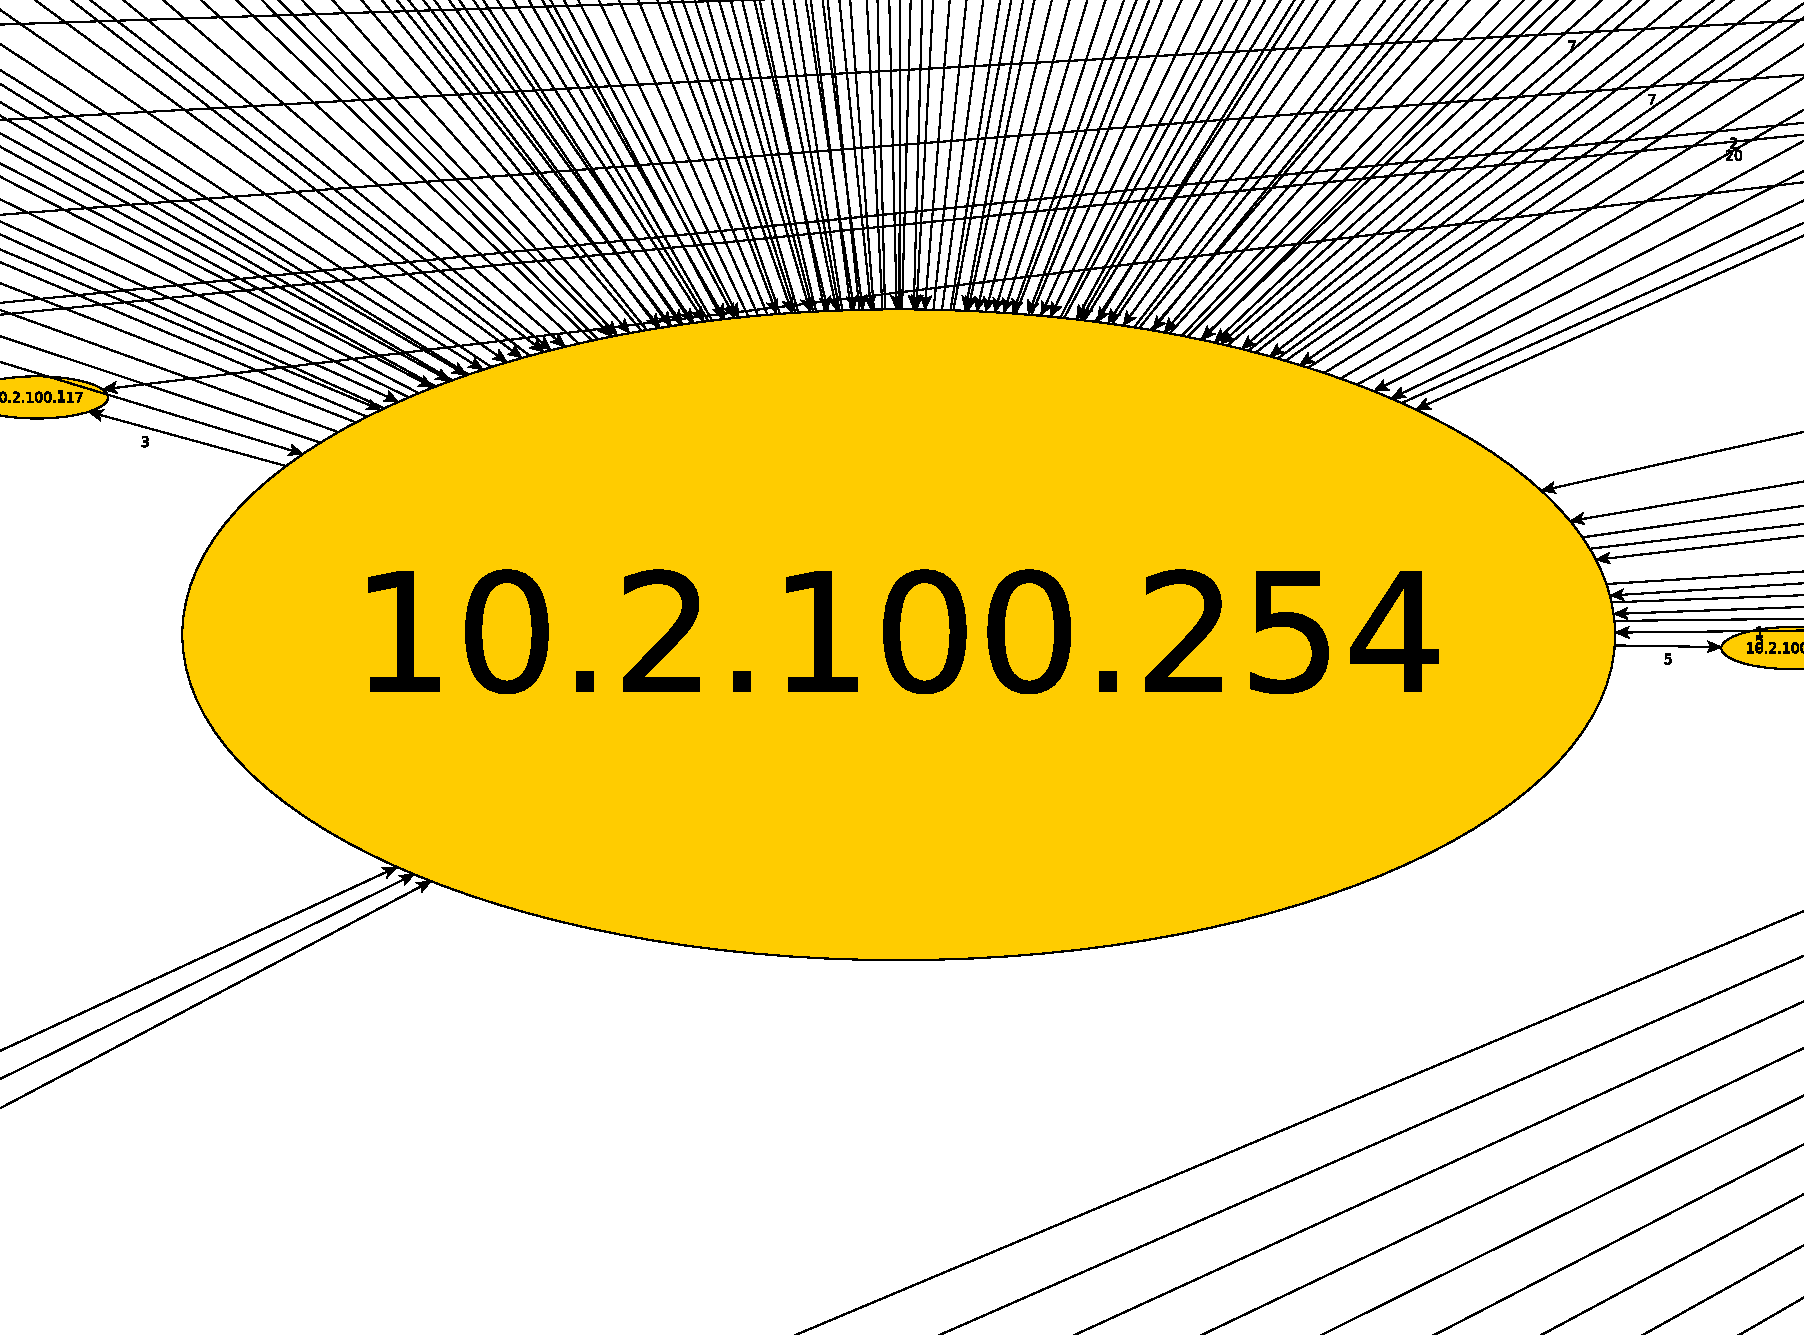
\includegraphics[width=0.45\textwidth, trim=0 0 0 0]{../Graficos/grafo_RedLabos_1_zoom_2.pdf}
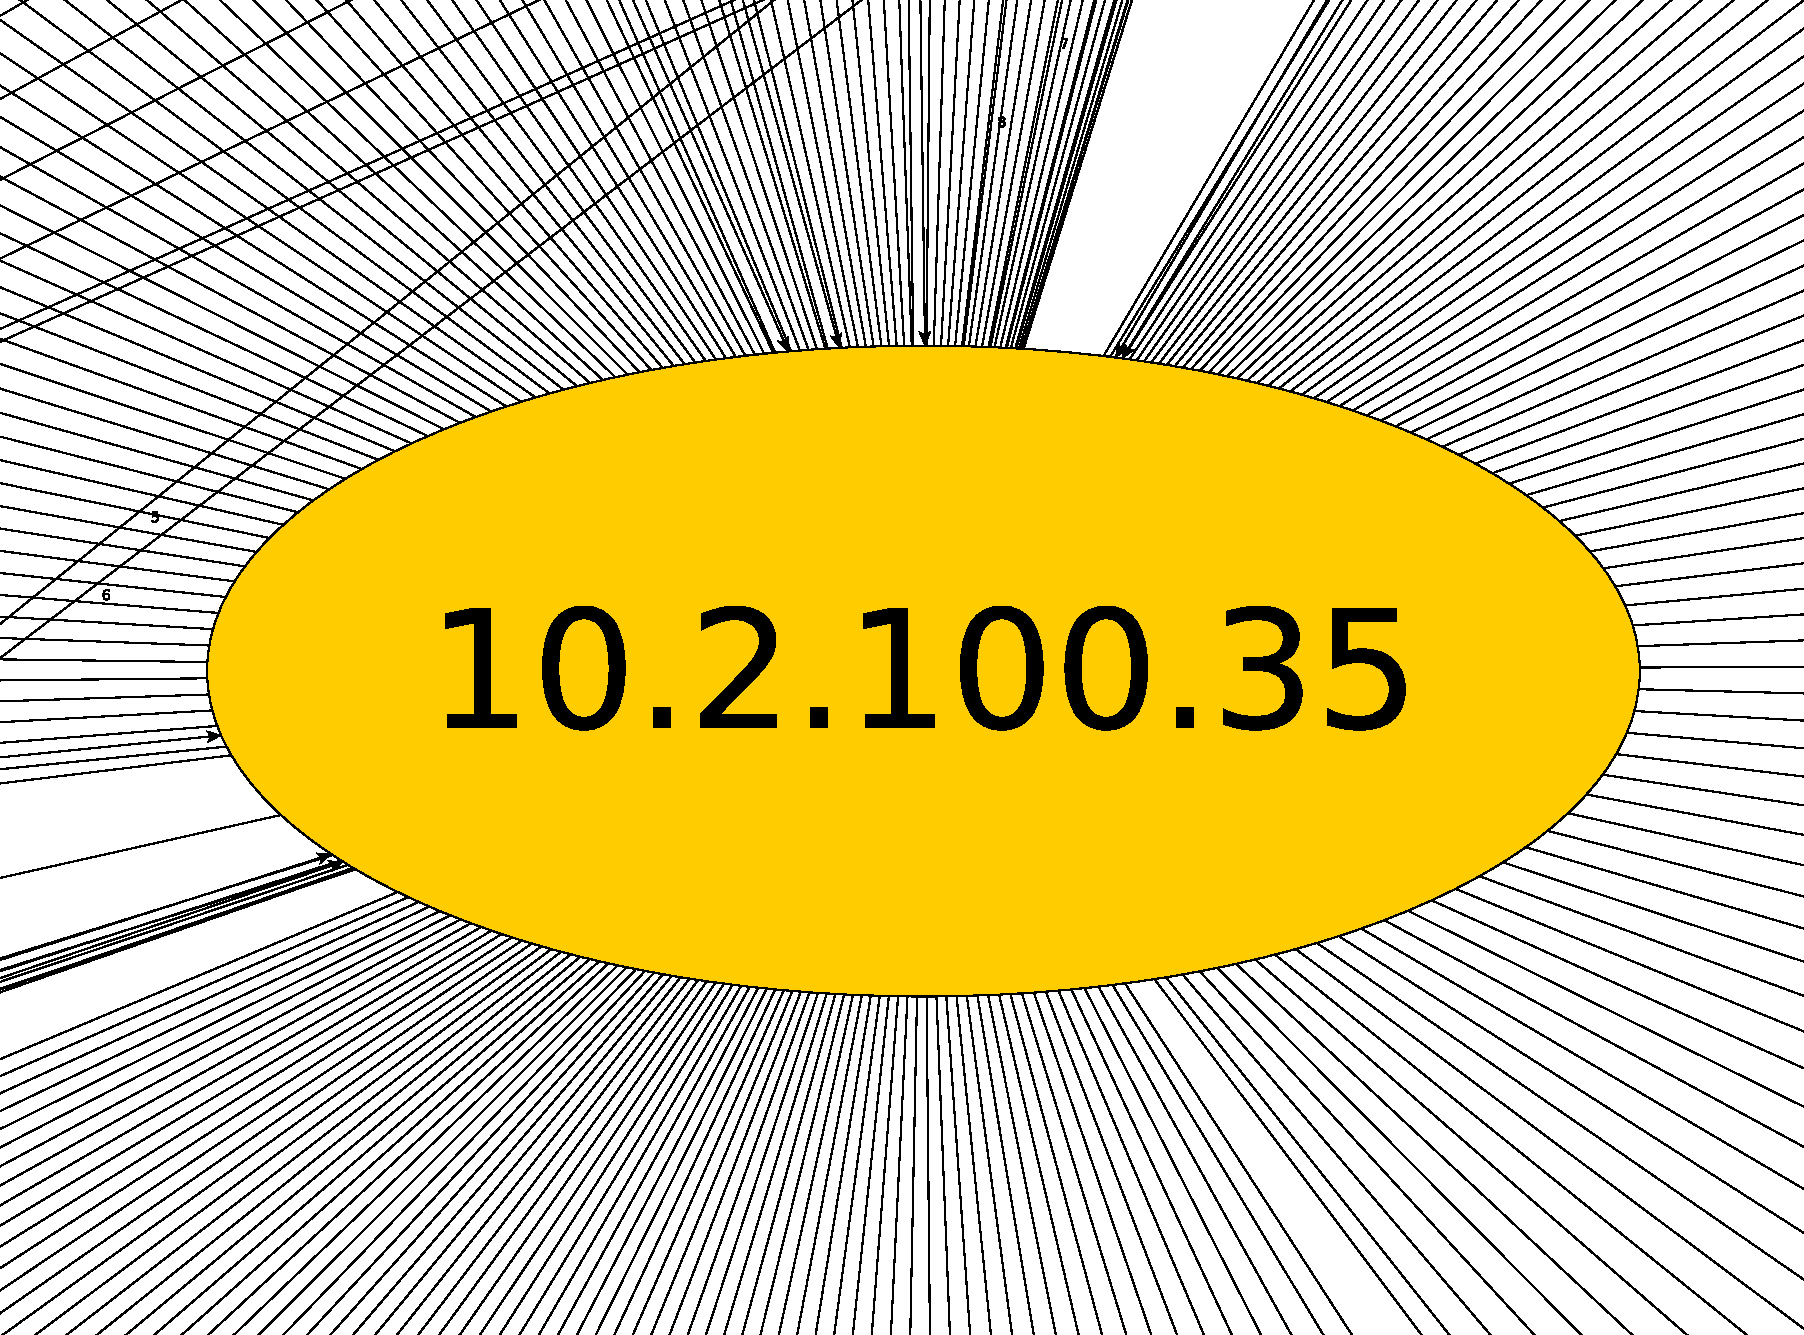
\includegraphics[width=0.45\textwidth, trim=0 0 0 0]{../Graficos/grafo_RedLabos_1_zoom_1.pdf}

\caption{Grafo de relaciones ARP en RedLabosDC durante 30 minutos de muestreo. Los nodos corresponden a IPs. Los ejes indican un envío de paquete
{\tt who-has} broadcast, relacionando IP fuente con IP destino. El peso de los ejes es la cantidad de paquetes capturados. Los grafos de menor tamaño
(derecha) se muestran ampliados en la Figura \ref{grafo-redlabos-2}.}
\label{grafo-redlabos-1}
\end{figure}

\newpage

\begin{figure}[h!]
\centering
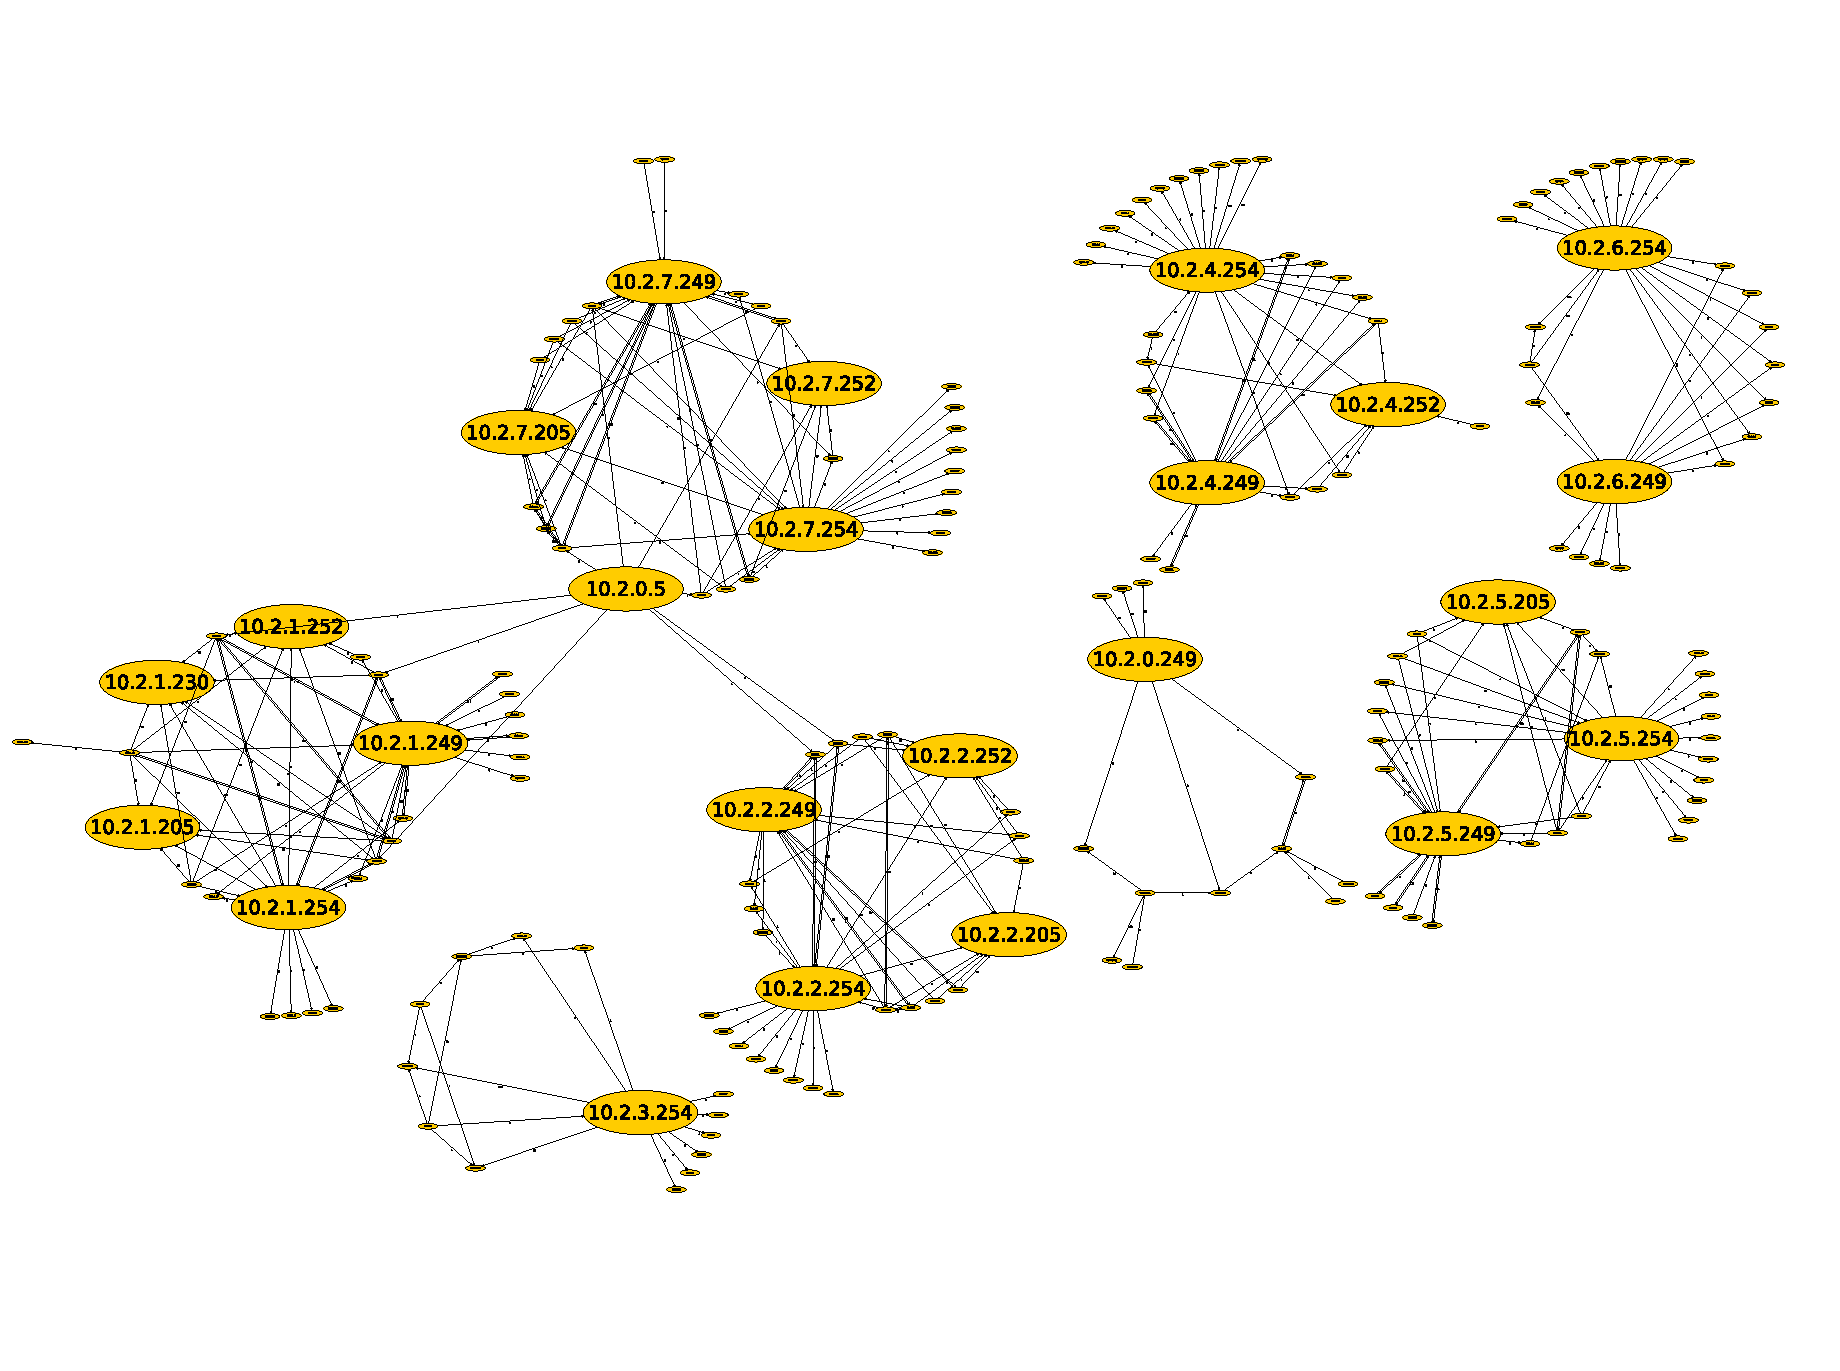
\includegraphics[width=\textwidth, trim=0 80 0 80]{../Graficos/grafo_RedLabos_1_zoom_3.pdf}

\fbox{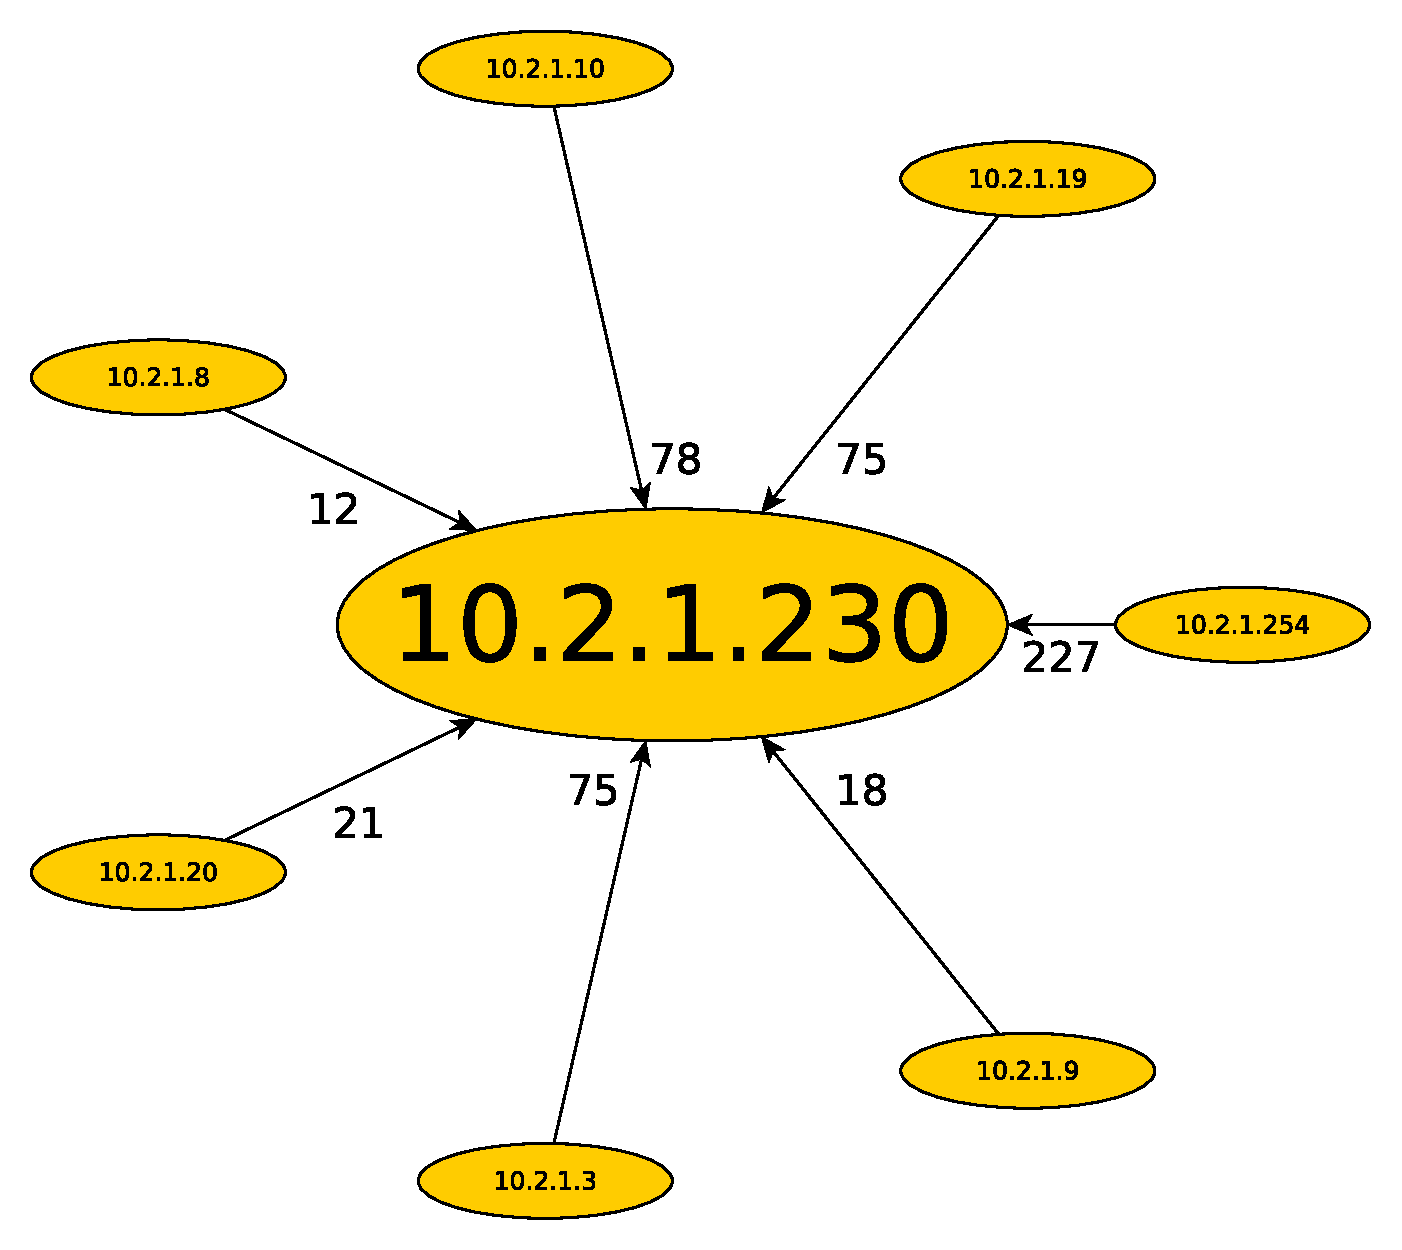
\includegraphics[width=0.5\textwidth, trim=0 0 0 0]{../Graficos/grafo_RedLabos_1_zoom_4.pdf}}

\caption{Grafo de relaciones ARP en RedLabosDC ampliado (Figura \ref{grafo-redlabos-1}). Los nodos corresponden a IPs. Los ejes indican un envío de paquete
{\tt who-has} broadcast, relacionando IP fuente con IP destino. El peso de los ejes es la cantidad de paquetes capturados. En el recuadro inferior se
muestra una ampliación de un sector para distinguir el peso de los ejes.}
\label{grafo-redlabos-2}
\end{figure}

\newpage

\begin{figure}[h!]
\centering
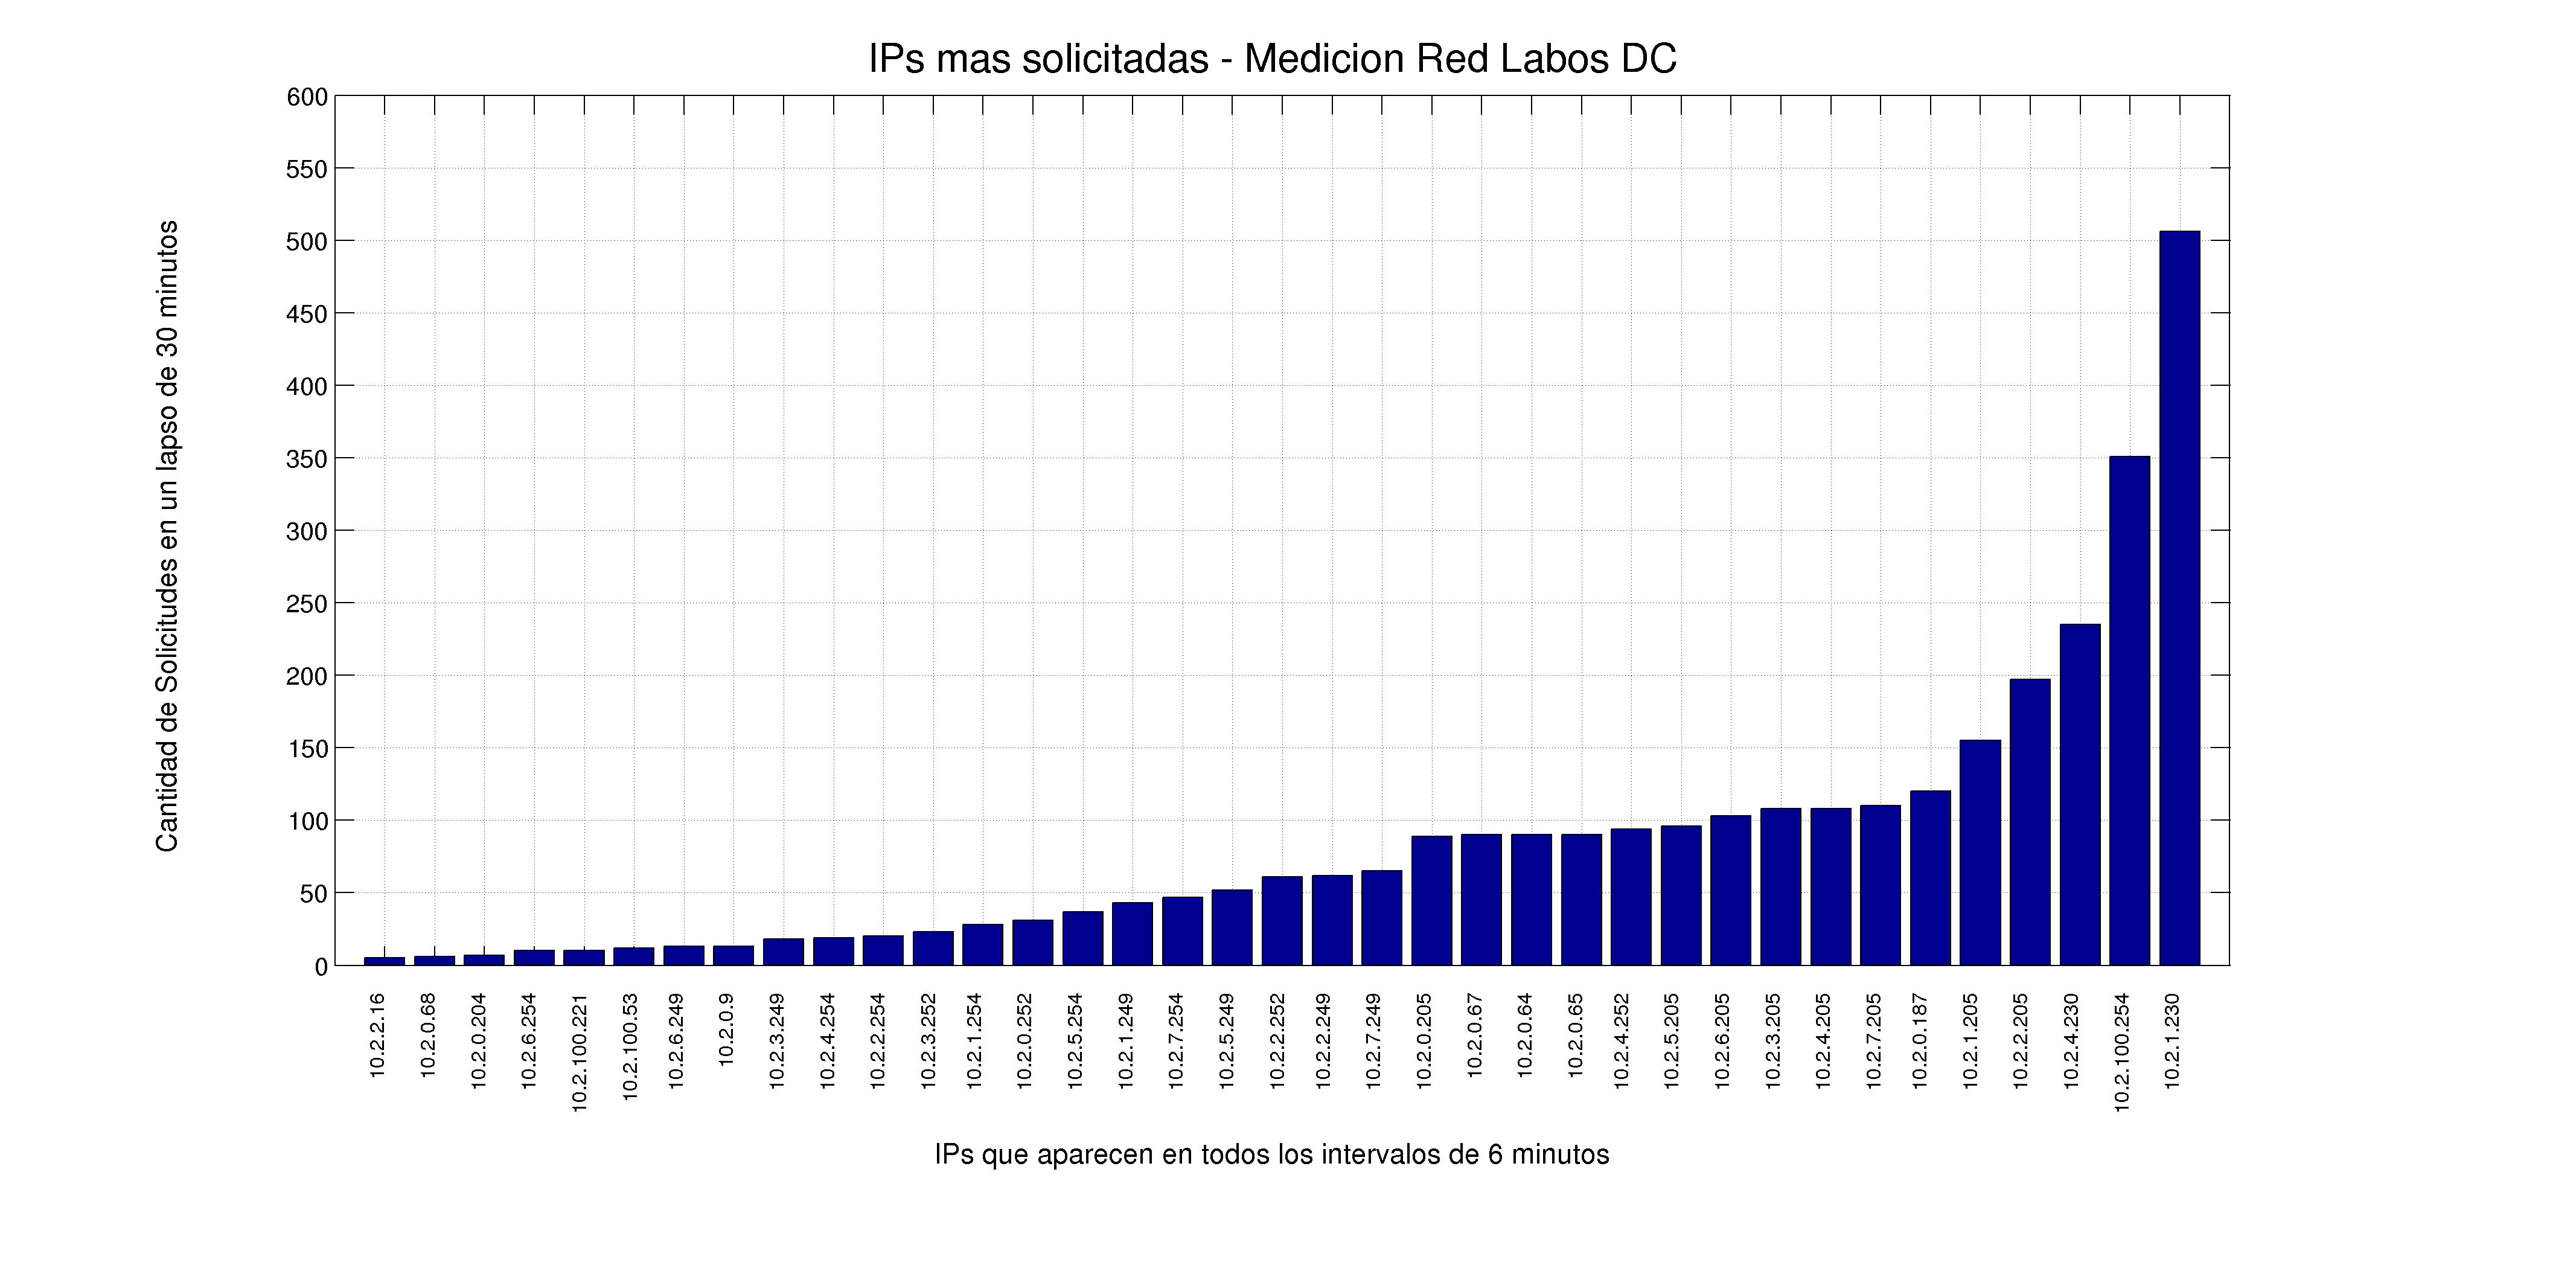
\includegraphics[width=\textwidth, trim=0 0 0 0]{../Graficos/ips_solicitadas_RedLabos_6.png}

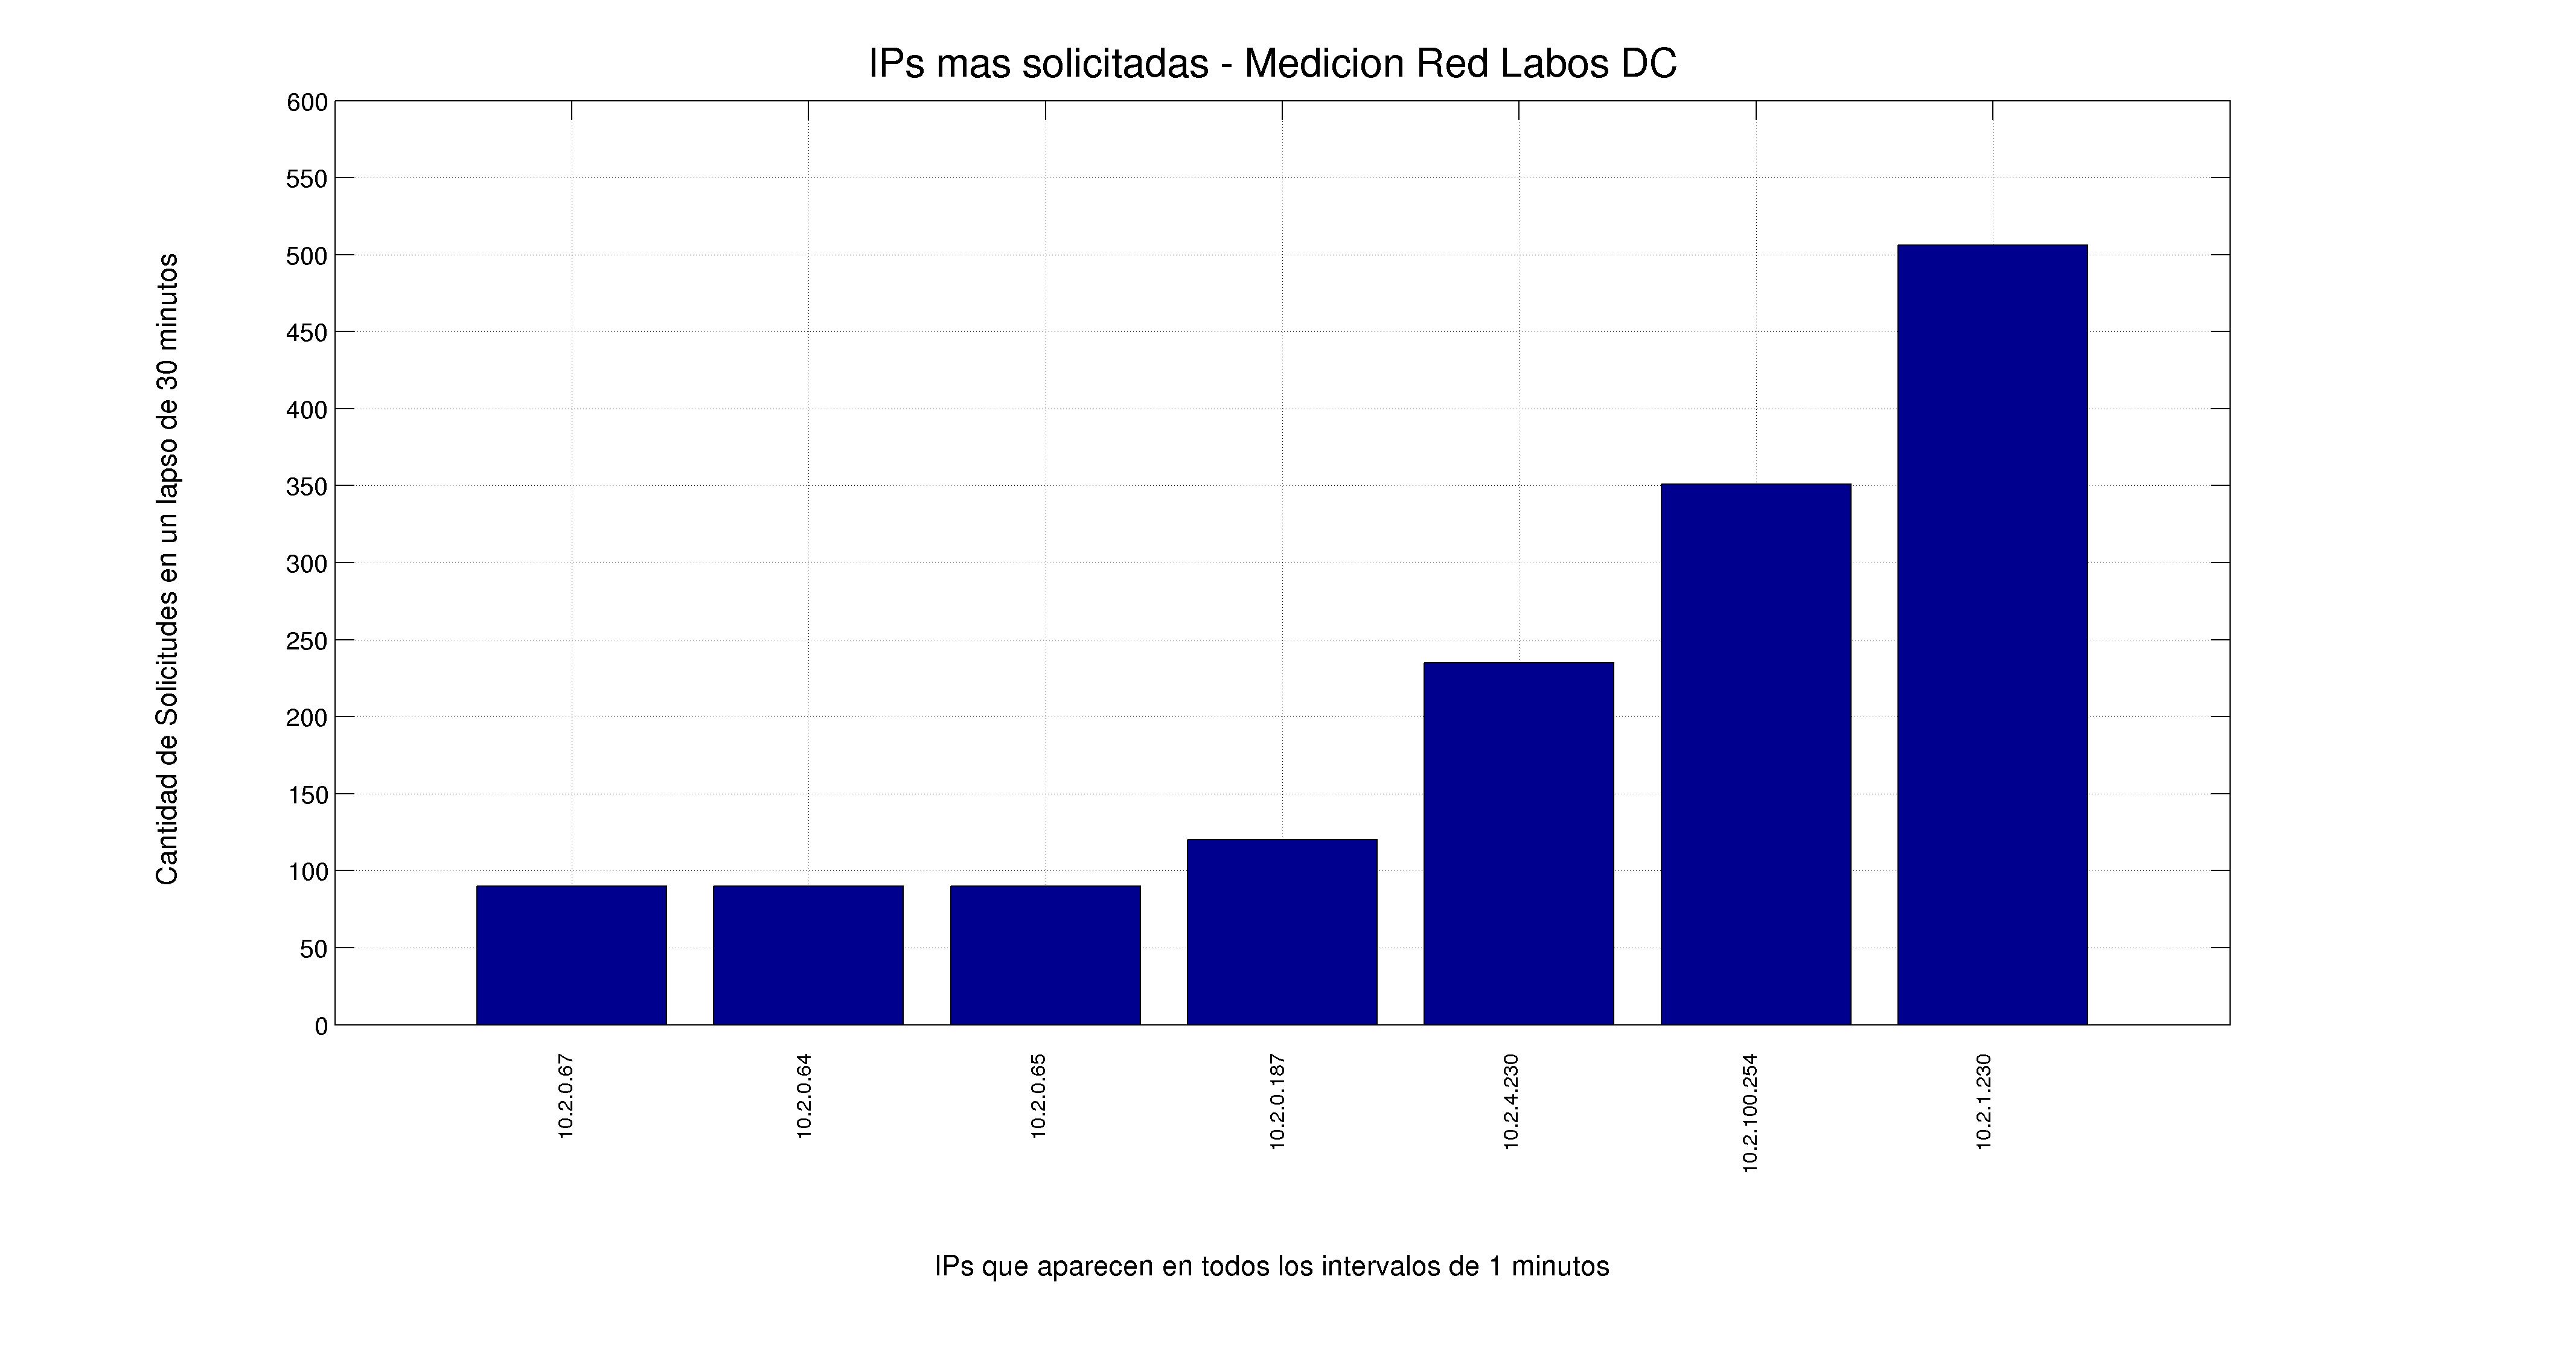
\includegraphics[width=\textwidth, trim=0 0 0 0]{../Graficos/ips_solicitadas_RedLabos_1.png}
\caption{IPs más solicitadas - Red Labos DC - Intervalos de 6 minutos y de 1 minuto. Las IPs mostradas son las que recibieron {\tt who-has} en todos los
intervalos de tiempo de dicha longitud, de la medición de 30 minutos. Una \emph{solicitud} corresponde a un paquete {\tt who-has} donde la IP aparecía
en el campo ARP\_IP\_DST.} \label{solicitadas-redlabos}
\end{figure}

\newpage

\begin{figure}[h!]
\centering
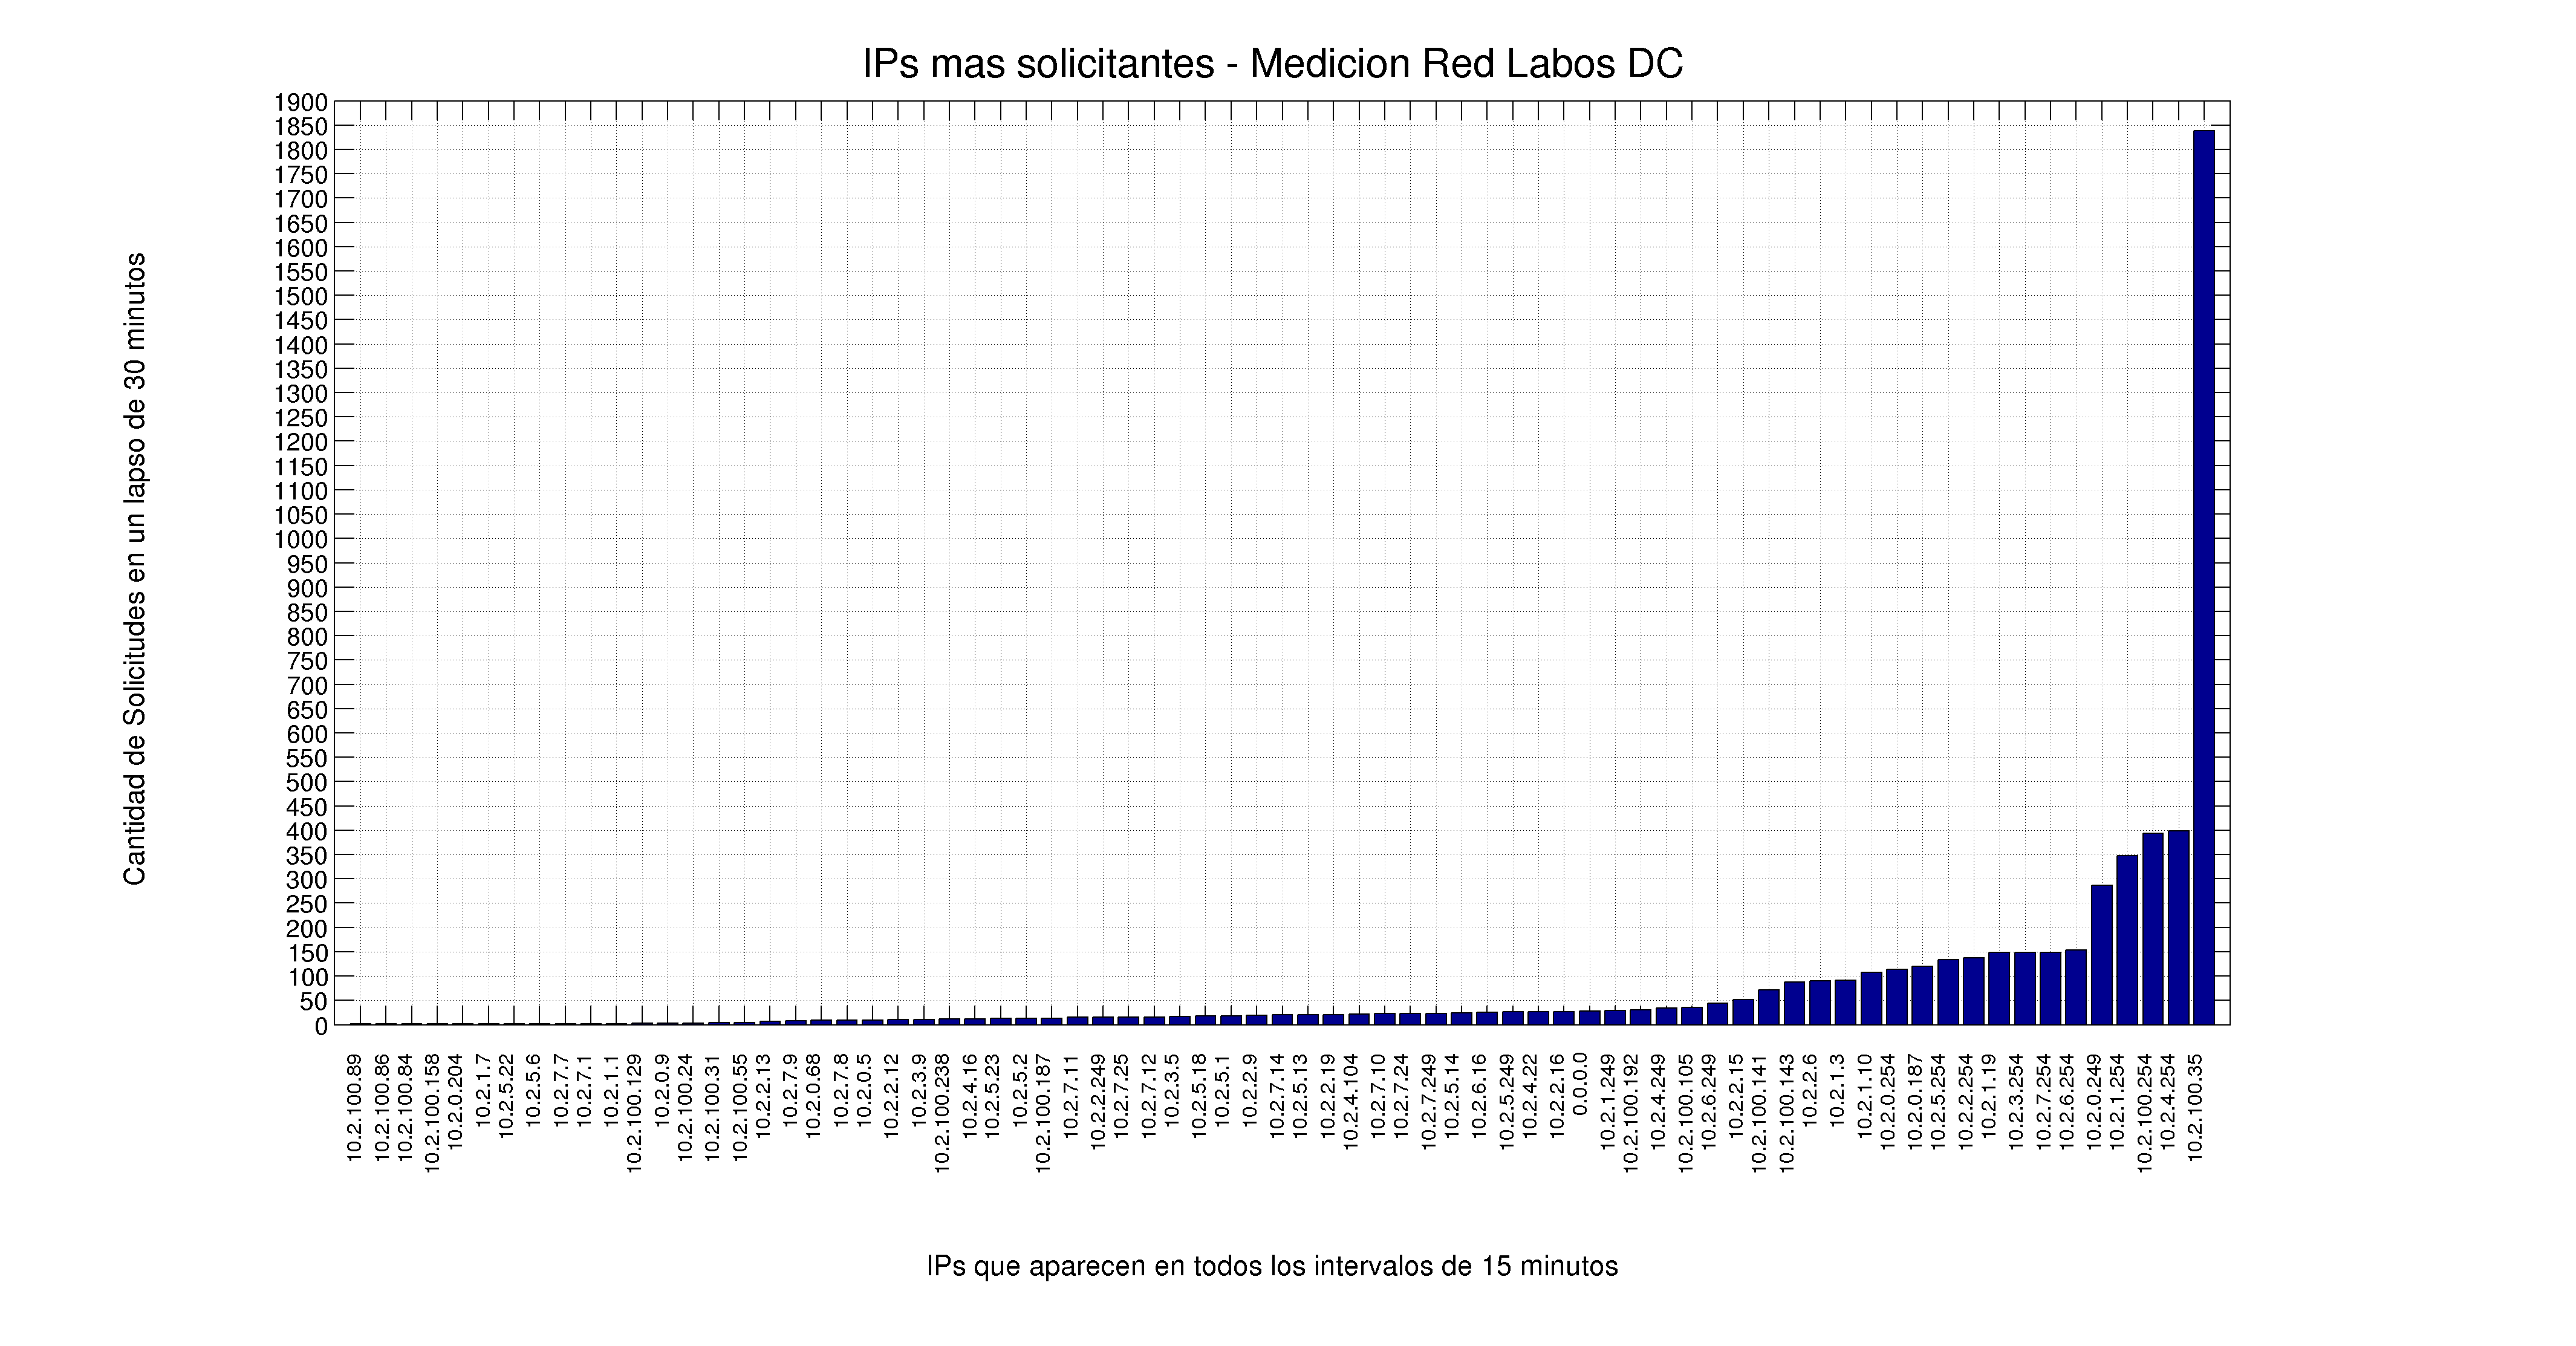
\includegraphics[width=\textwidth, trim=0 0 0 0]{../Graficos/ips_solicitantes_RedLabos_15.png}

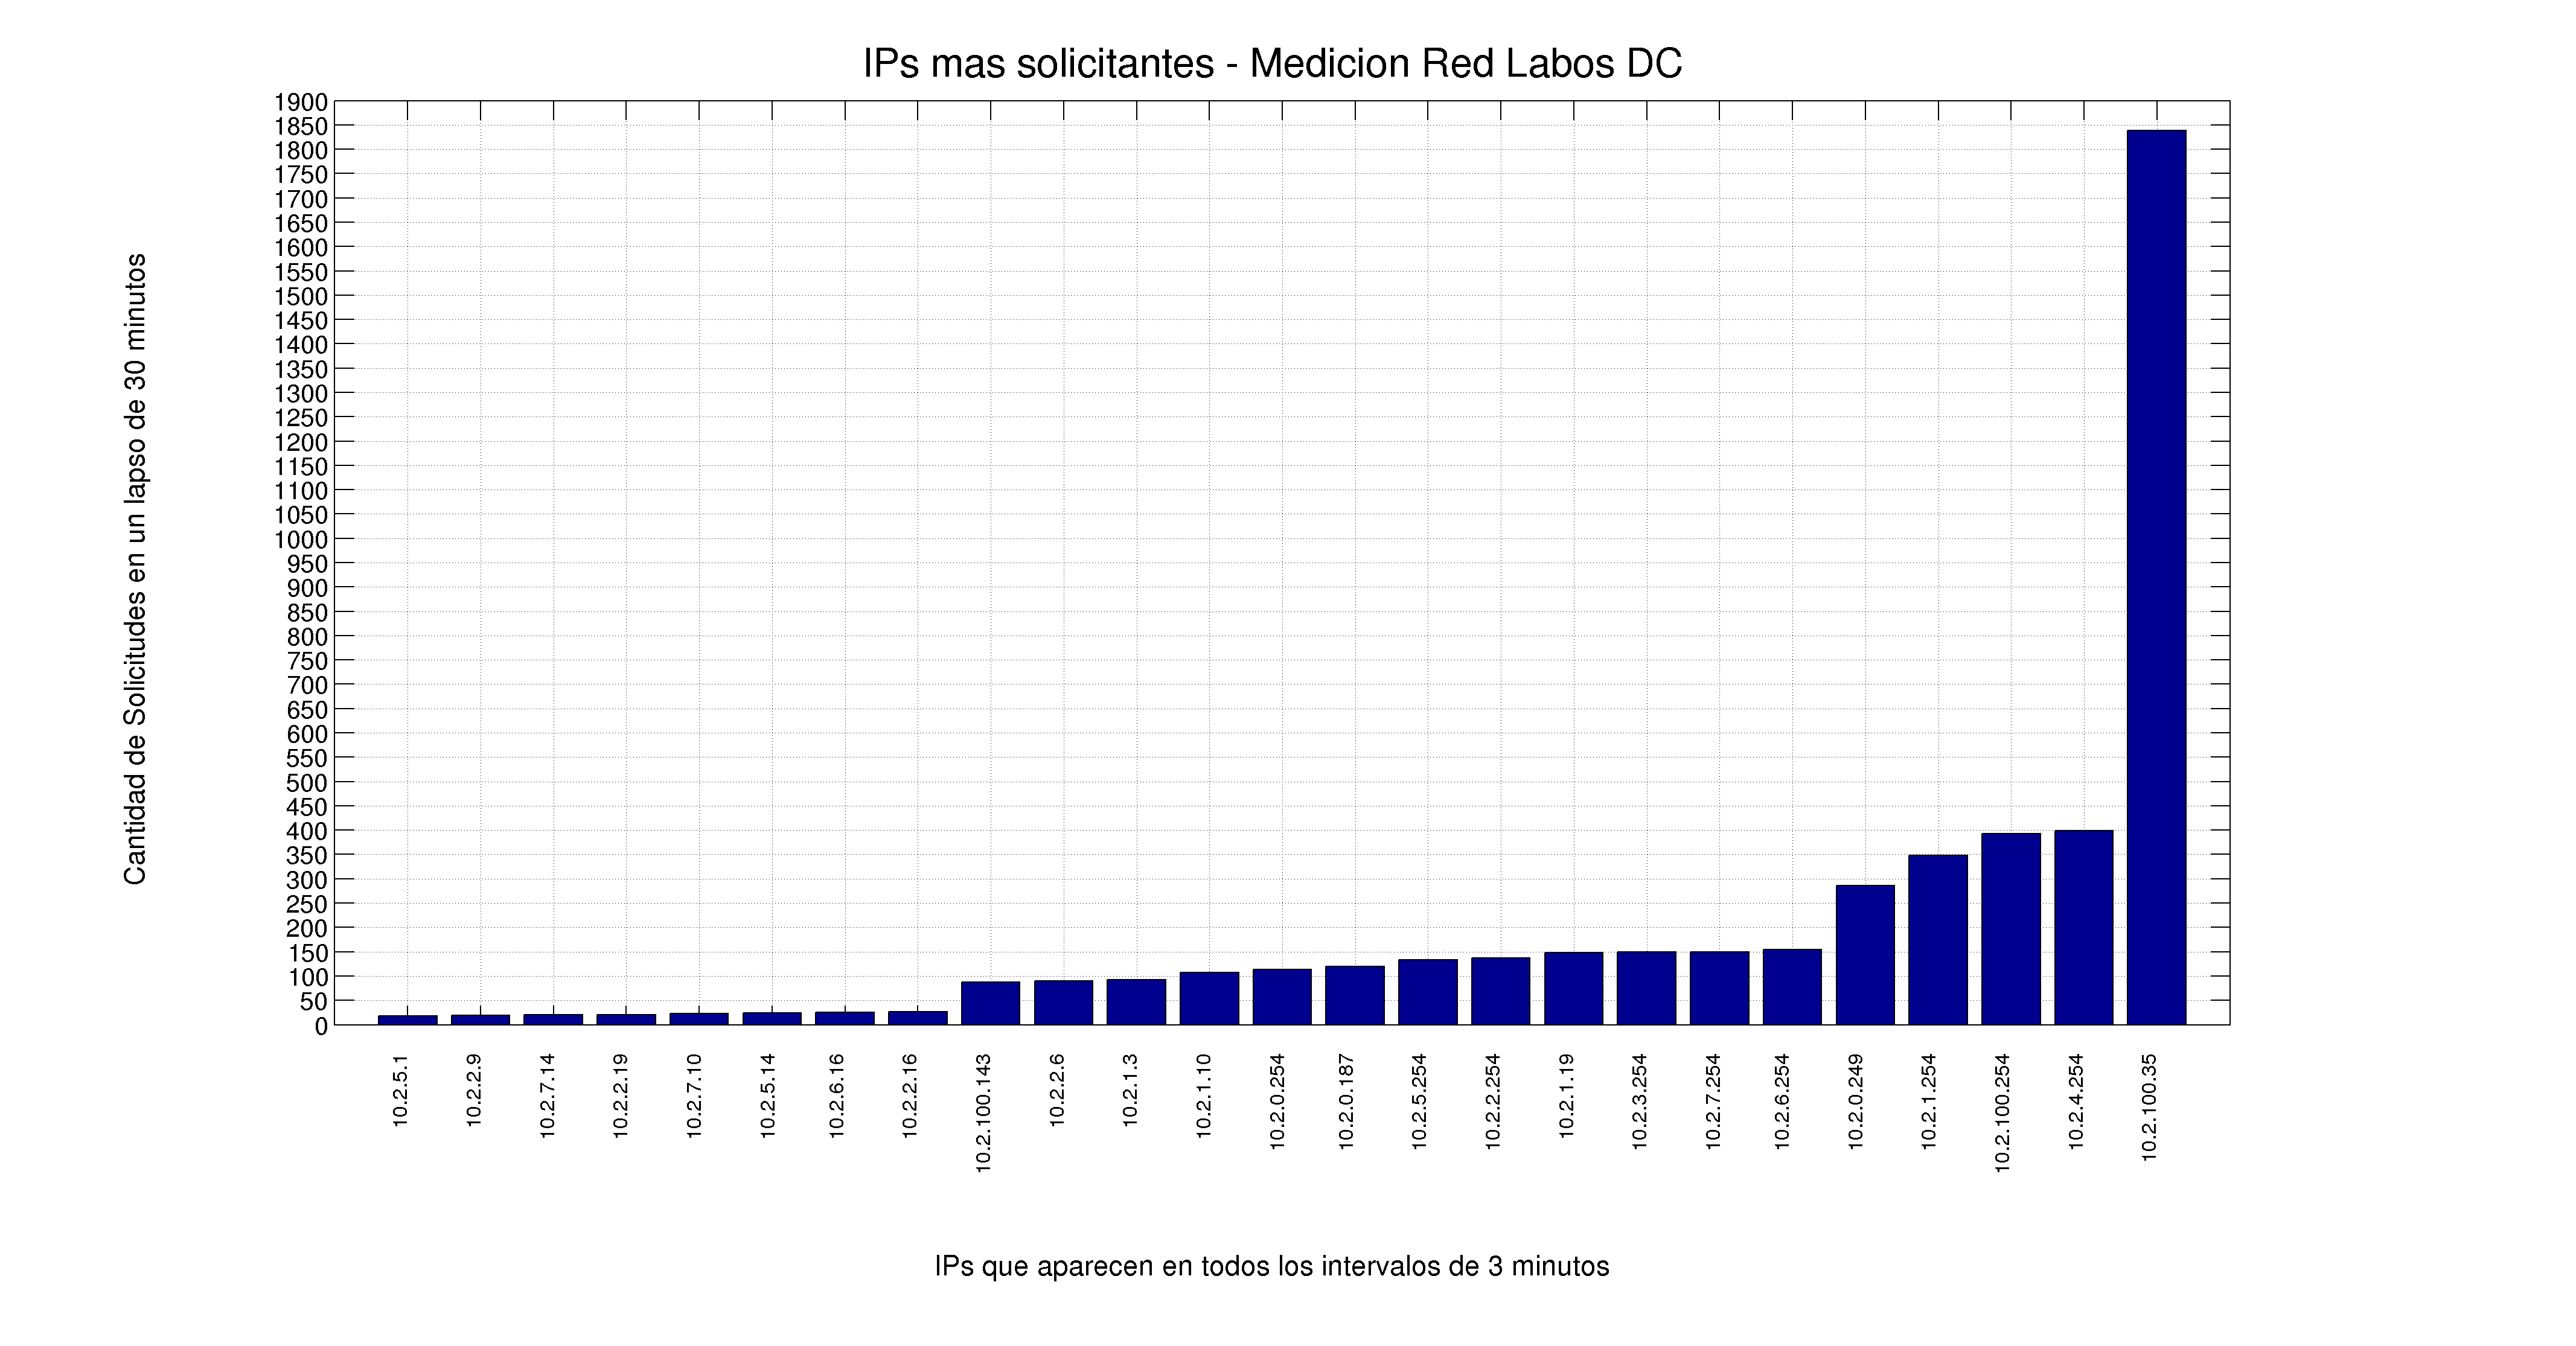
\includegraphics[width=\textwidth, trim=0 0 0 0]{../Graficos/ips_solicitantes_RedLabos_3.png}
\caption{IPs más solicitantes - Red Labos DC - Intervalos de 15 minutos y de 3 minutos. Las IPs mostradas son las que enviaron {\tt who-has} en todos los
intervalos de tiempo de dicha longitud, de la medición de 30 minutos. Una \emph{solicitud} corresponde a un paquete {\tt who-has} donde la IP aparecía
en el campo ARP\_IP\_SRC.} \label{solicitantes-redlabos}
\end{figure}

\newpage

\begin{figure}[h!]
\centering
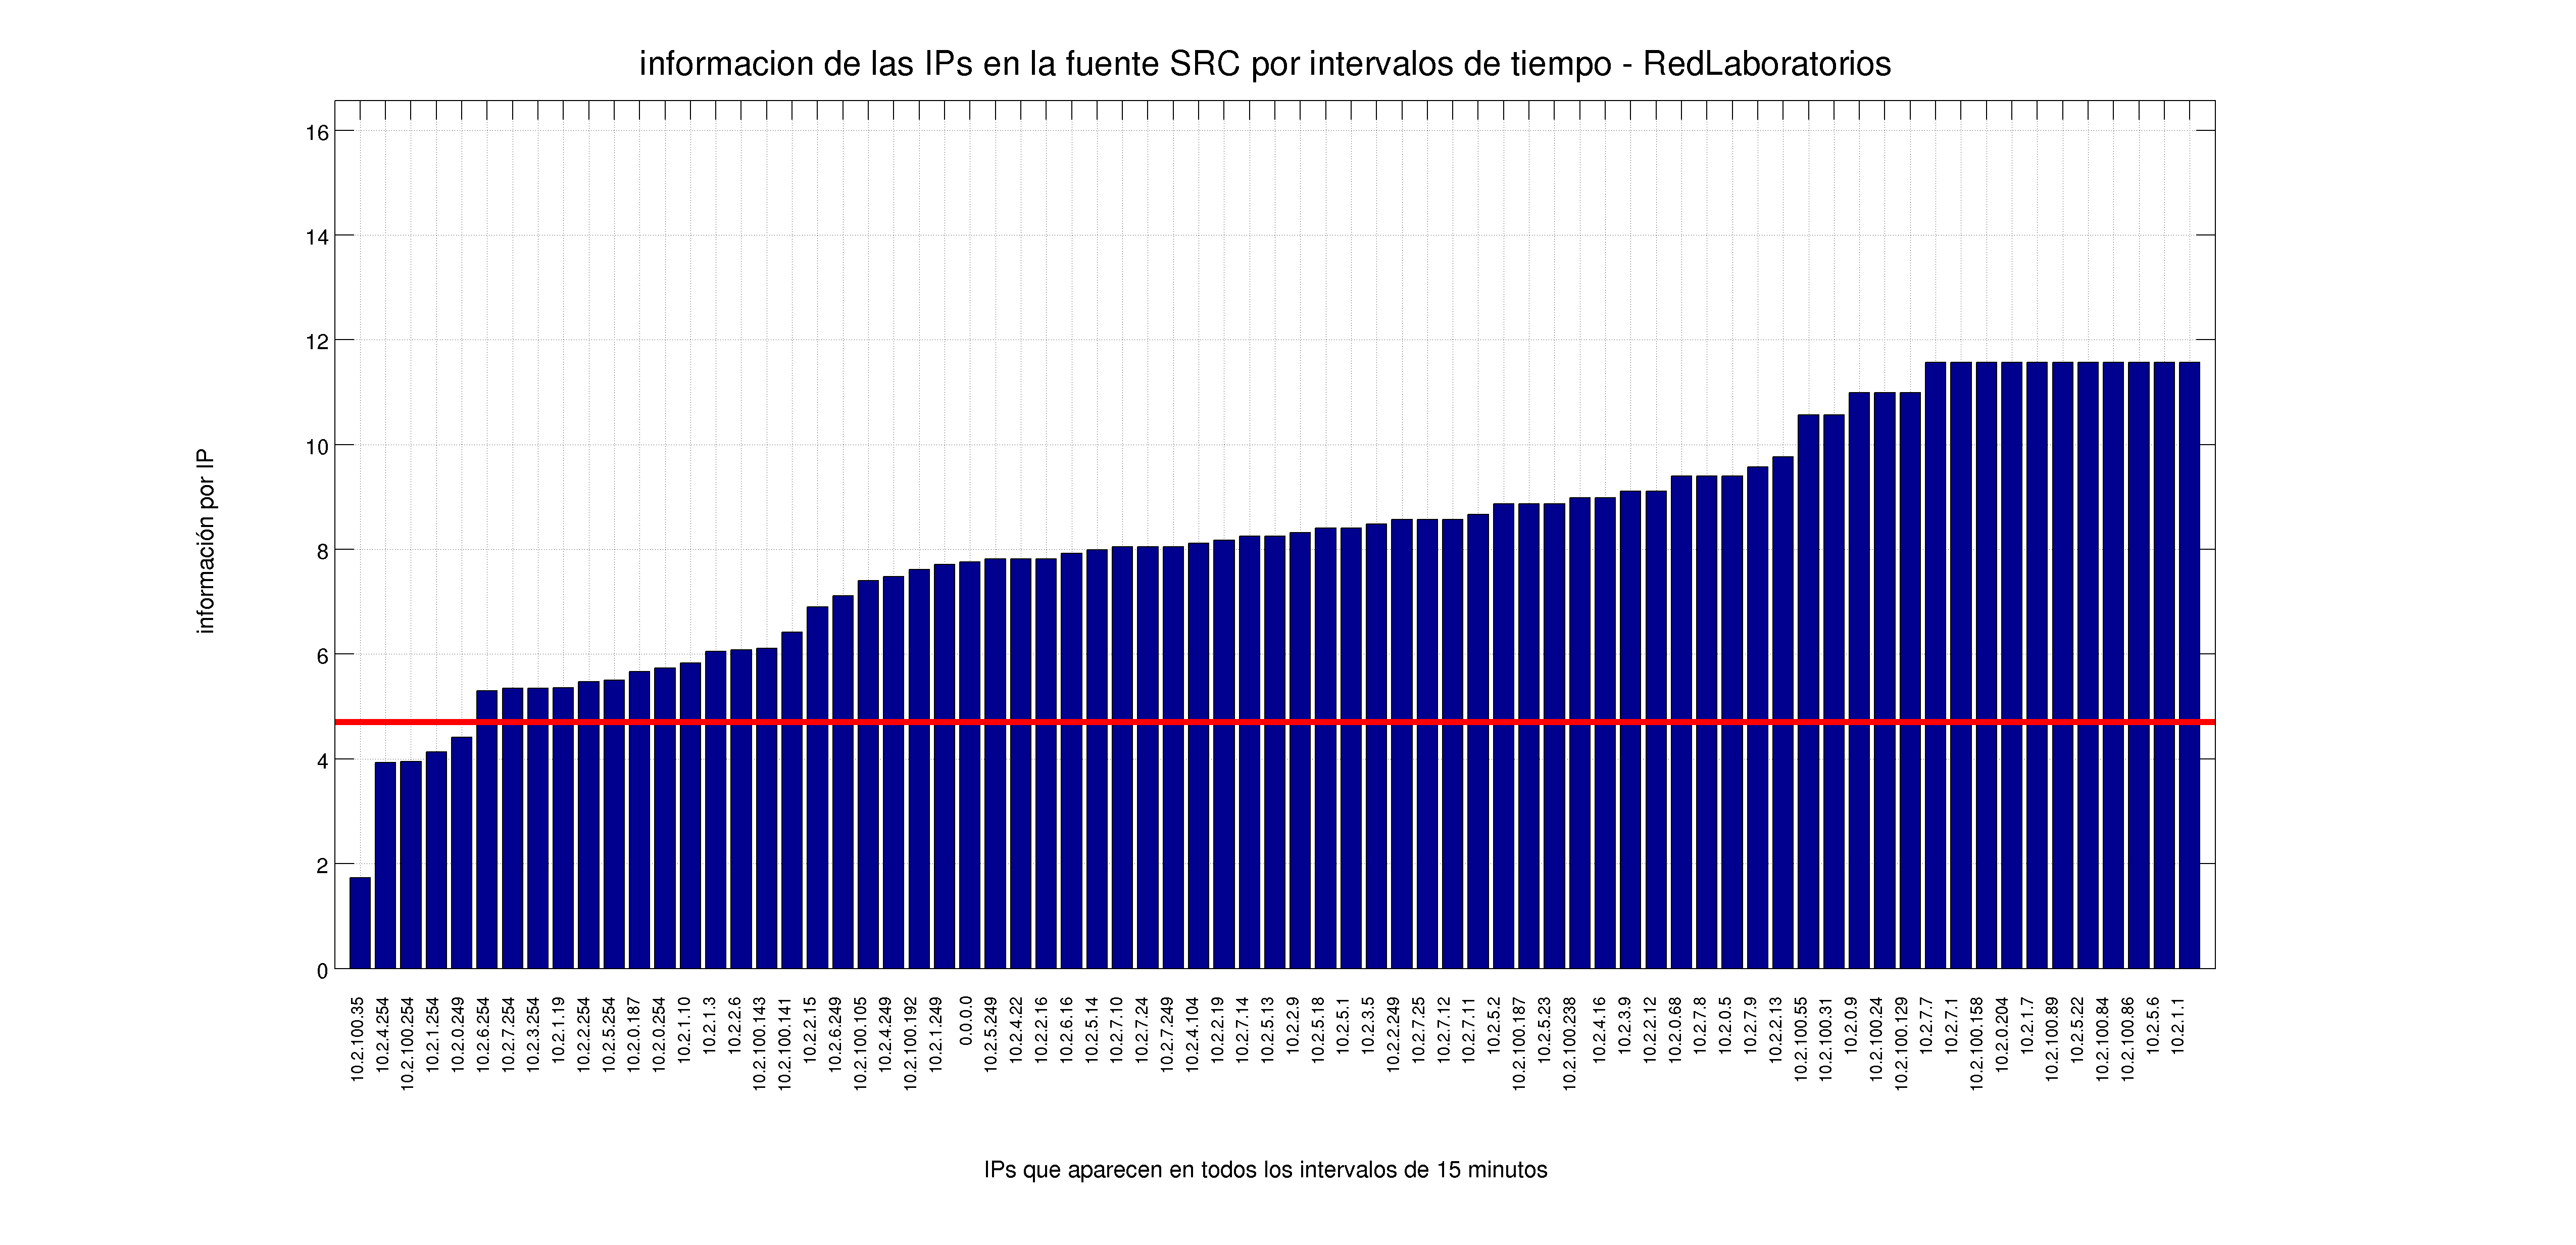
\includegraphics[width=\textwidth, trim=0 0 0 0]{../Graficos/labos_infoConEn_15.png}

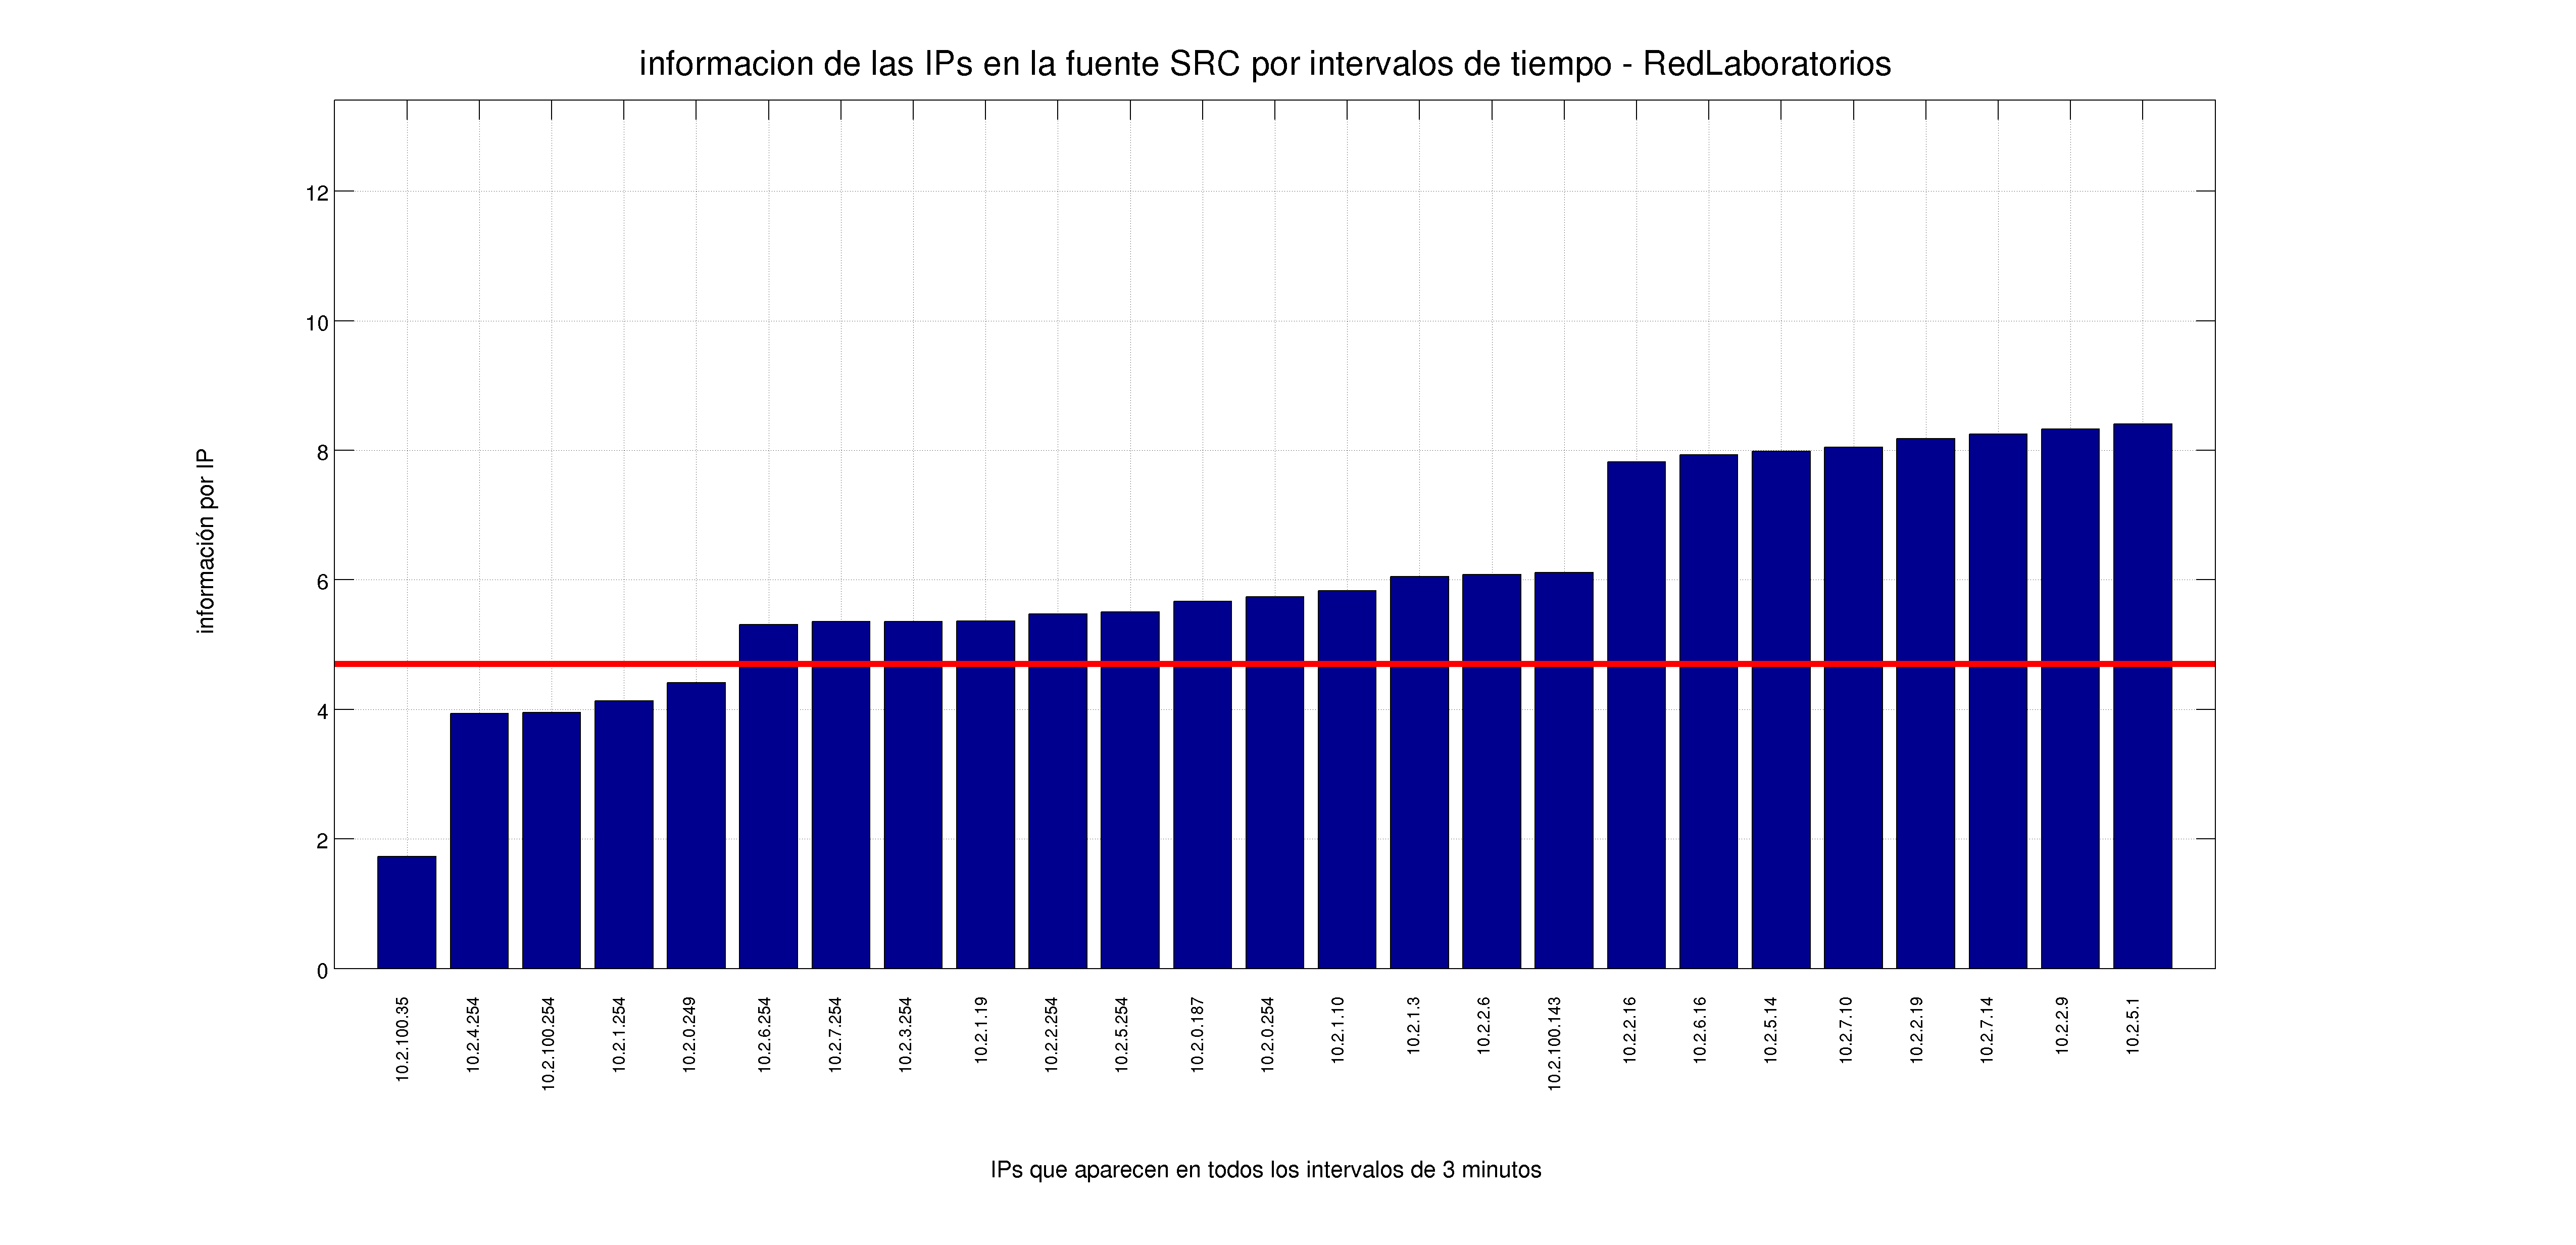
\includegraphics[width=\textwidth, trim=0 0 0 0]{../Graficos/labos_infoConEn_3.png}
\caption{Información y Entropía (rojo) - Fuente $S_{src}$ - Red Labos DC - Intervalos de 15 minutos y de 3 minutos. Las IPs mostradas son las que enviaron {\tt who-has} en todos los
intervalos de tiempo de dicha longitud, de la medición de 30 minutos.}
\end{figure}


\newpage

\begin{figure}[h!]
\centering
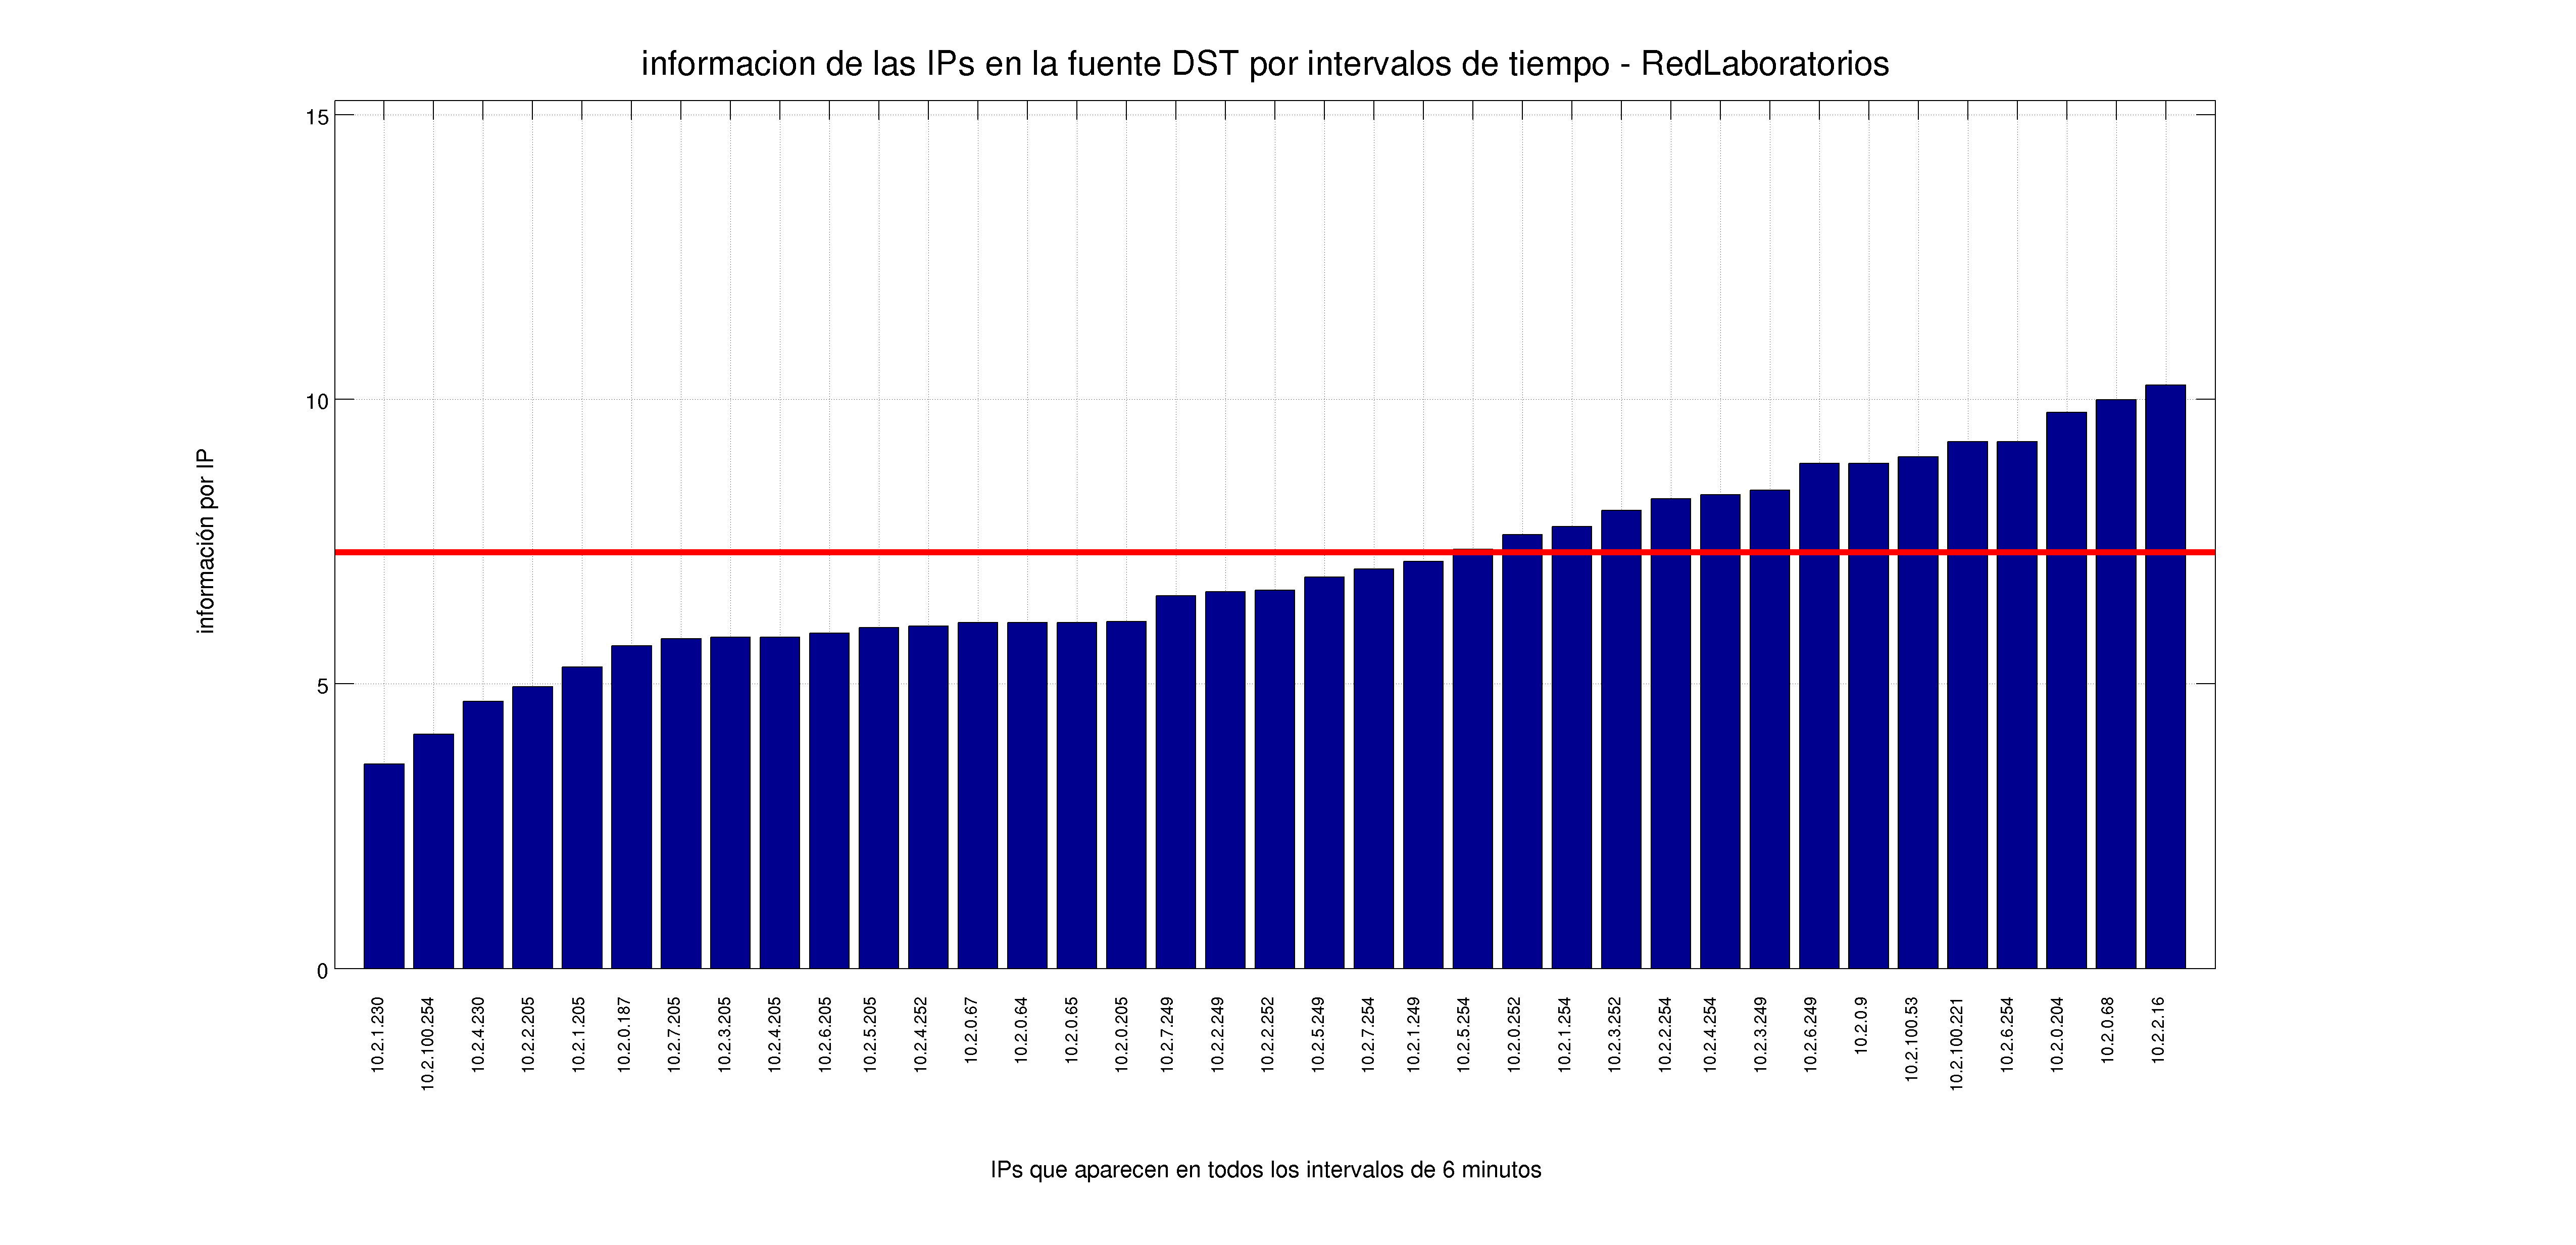
\includegraphics[width=\textwidth, trim=0 0 0 0]{../Graficos/labos_infoConEn_dst_6.png}

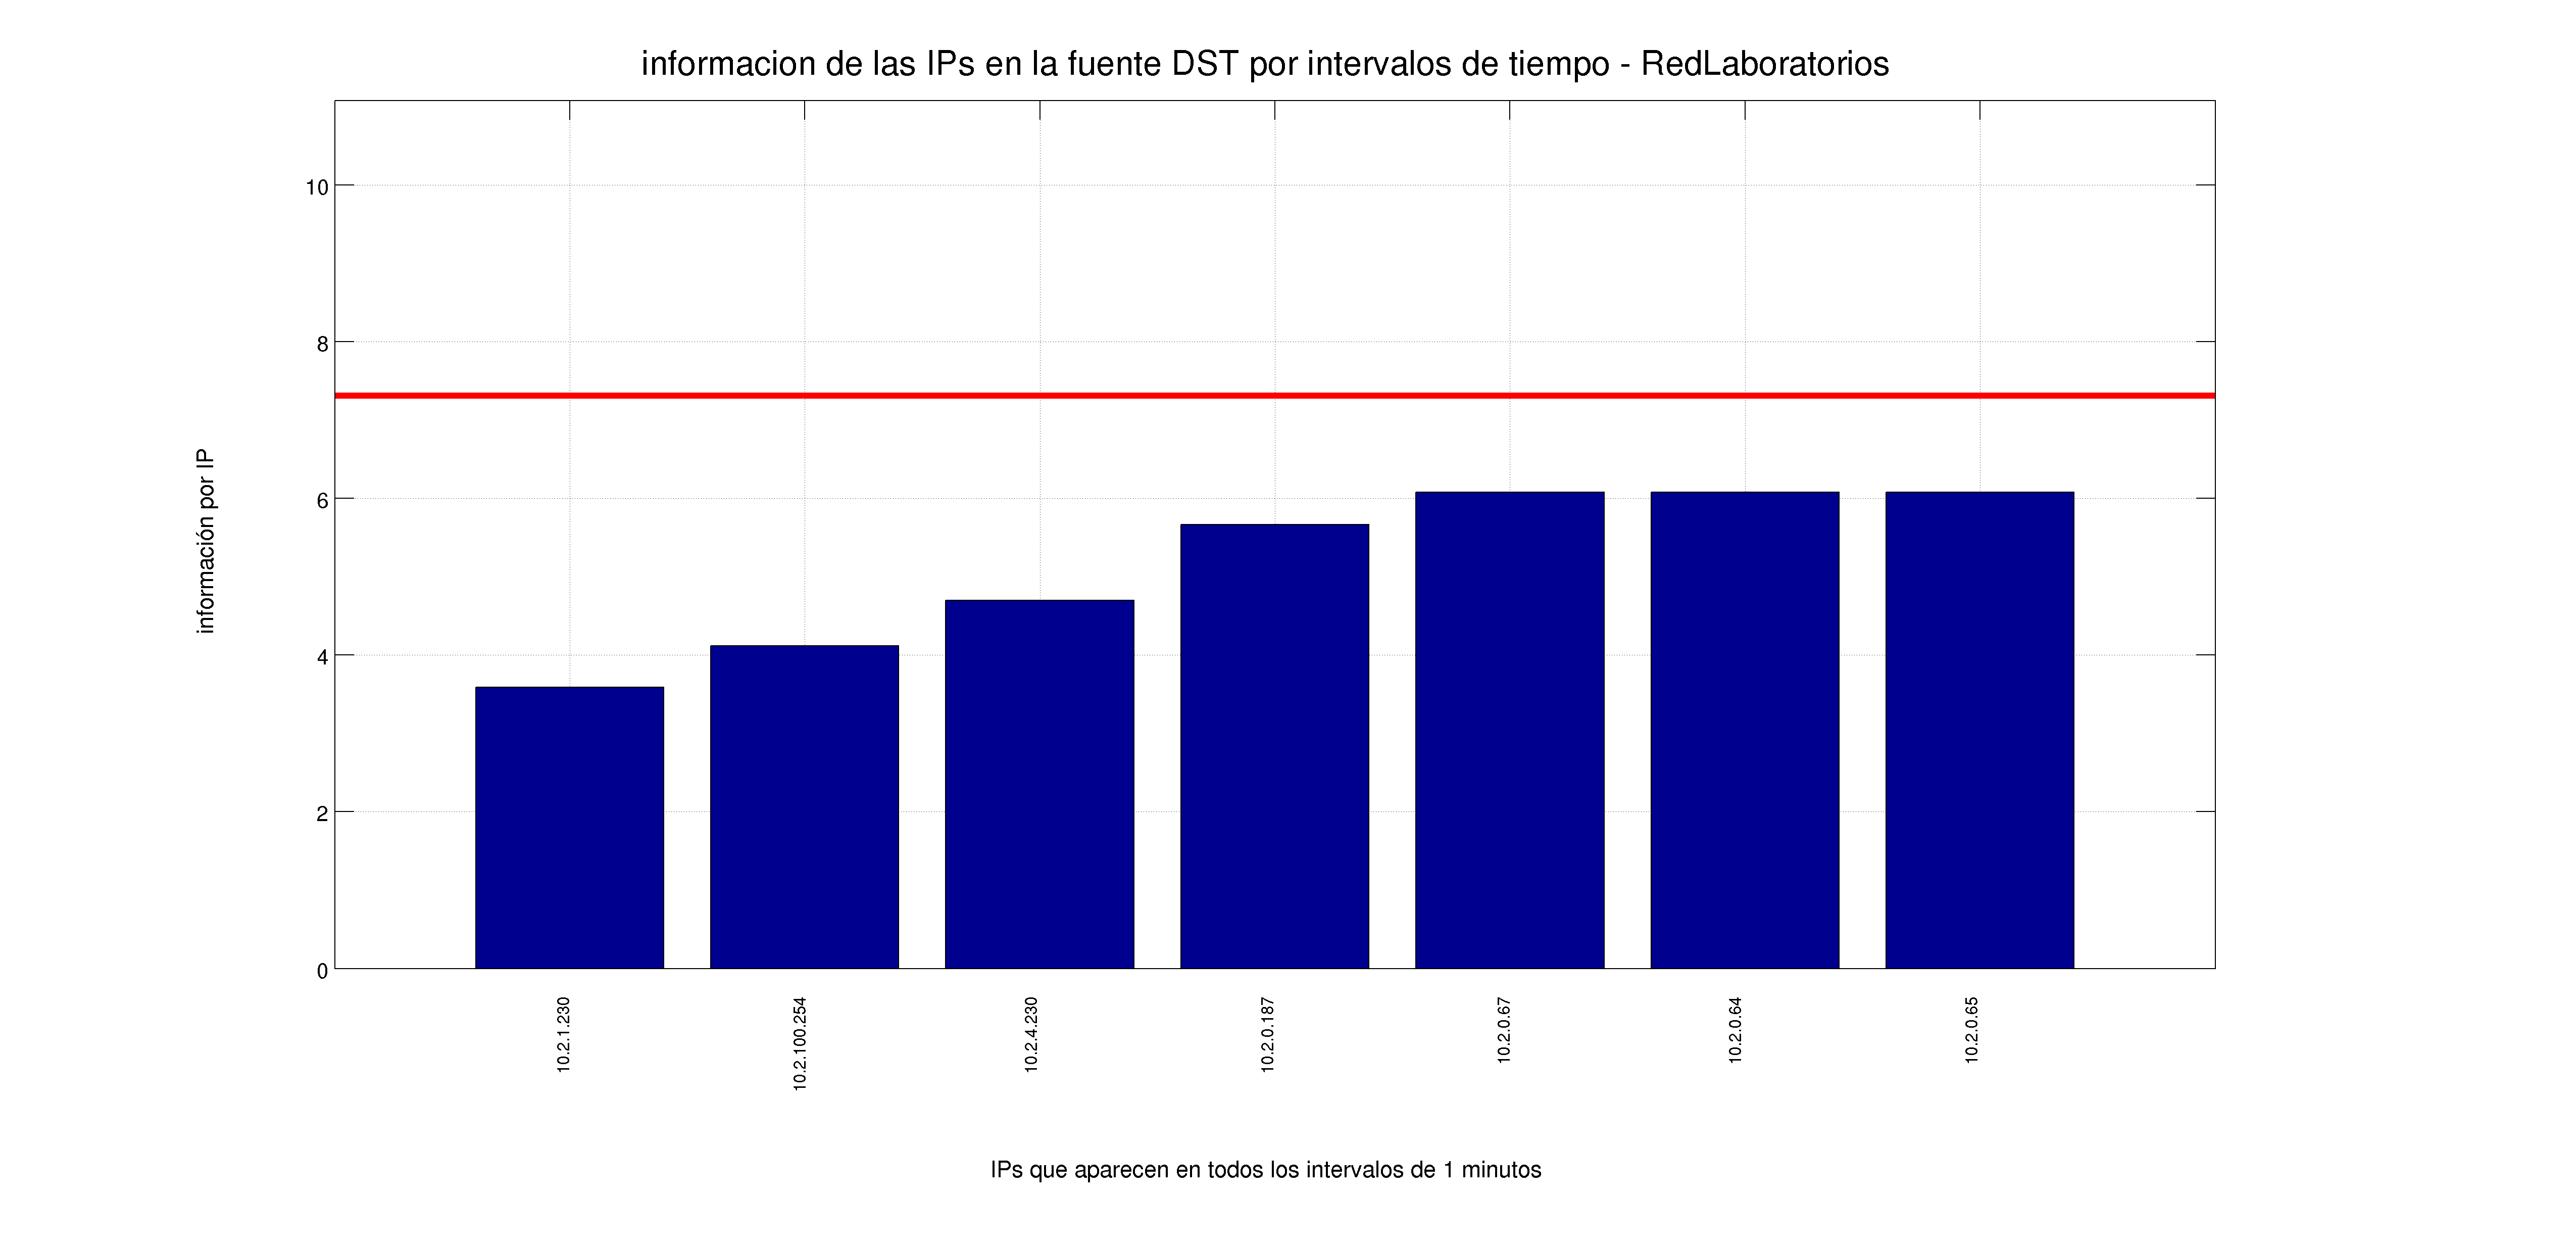
\includegraphics[width=\textwidth, trim=0 0 0 0]{../Graficos/labos_infoConEn_dst_1.png}
\caption{Información y Entropía (rojo) - Fuente $S_{dst}$ - Red Labos DC - Intervalos de 6 minutos y de 1 minutos. Las IPs mostradas son las que enviaron {\tt who-has} en todos los
intervalos de tiempo de dicha longitud, de la medición de 30 minutos.}
\end{figure}

\newpage


\subsection{Red Entrepiso}

\begin{figure}[h!]
\centering
\includegraphics[width=1\textwidth, trim=0 0 0 0]{../Graficos/grafo_Entrepiso.pdf}
\caption{Grafo de relaciones ARP en RedEntrepiso durante 30 minutos de muestreo. Los nodos corresponden a IPs. Los ejes indican un envío de paquete
{\tt who-has} broadcast, relacionando IP fuente con IP destino. El peso de los ejes es la cantidad de paquetes capturados.}
\end{figure}

\newpage

\begin{figure}[h!]
\centering
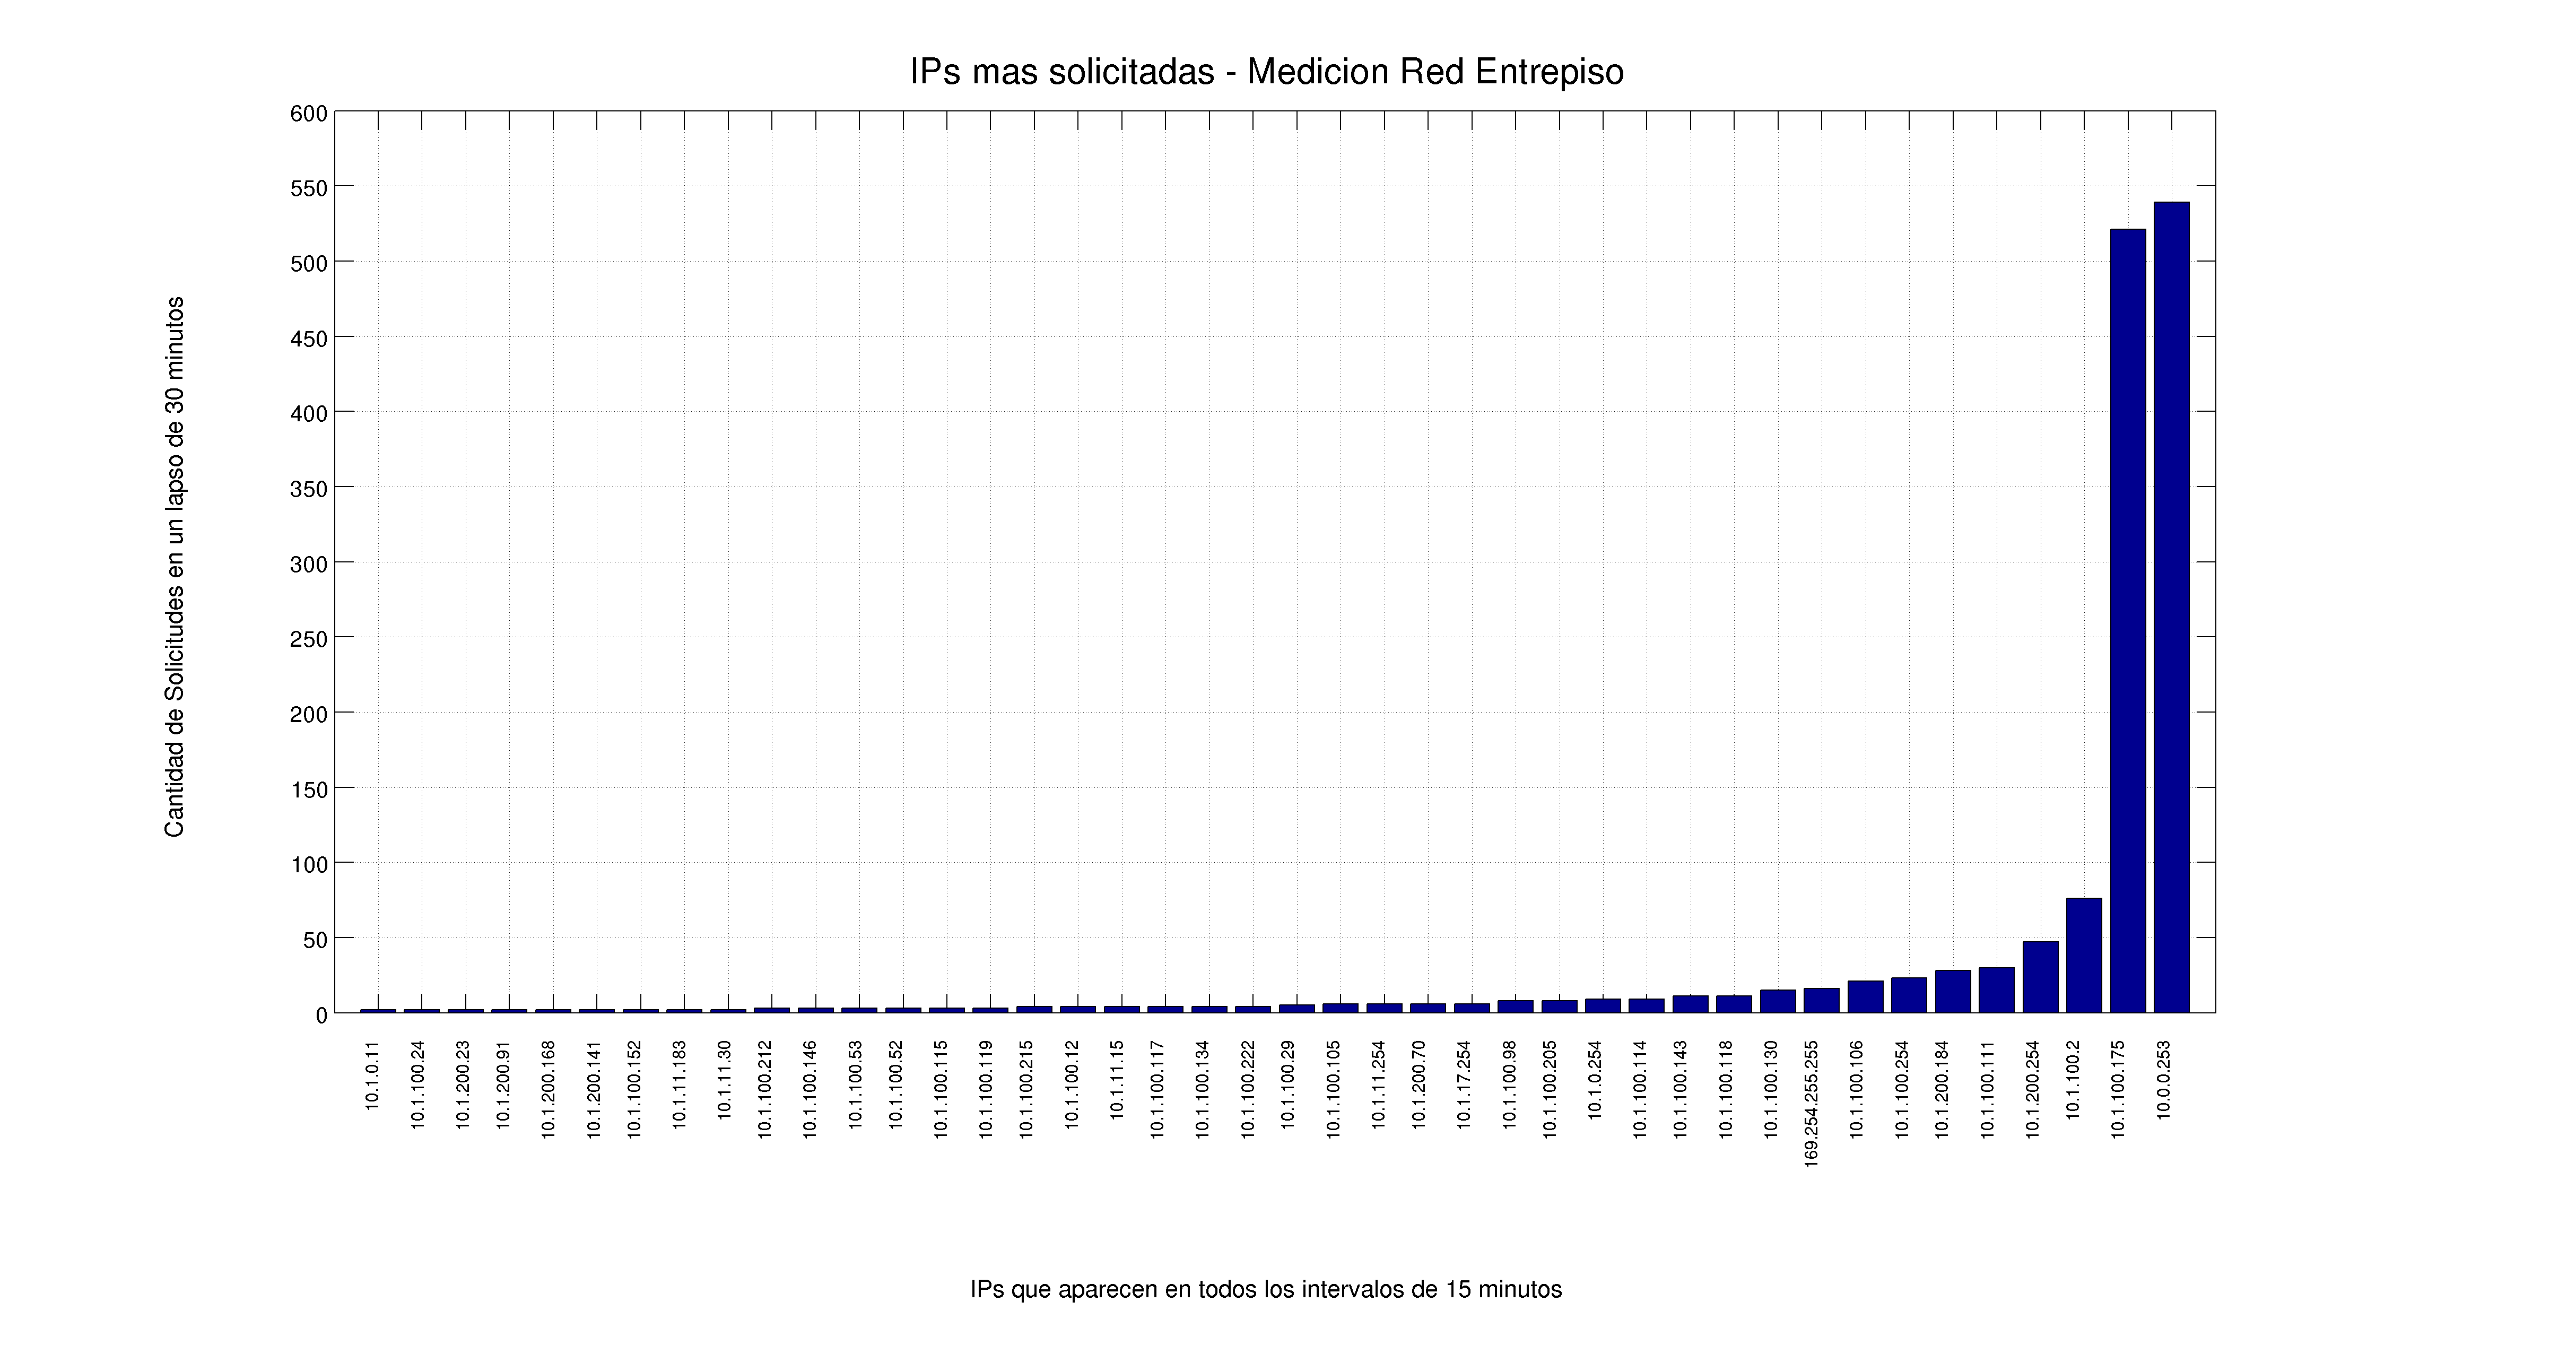
\includegraphics[width=\textwidth, trim=0 0 0 0]{../Graficos/ips_solicitadas_RedEntrepiso_15.png}

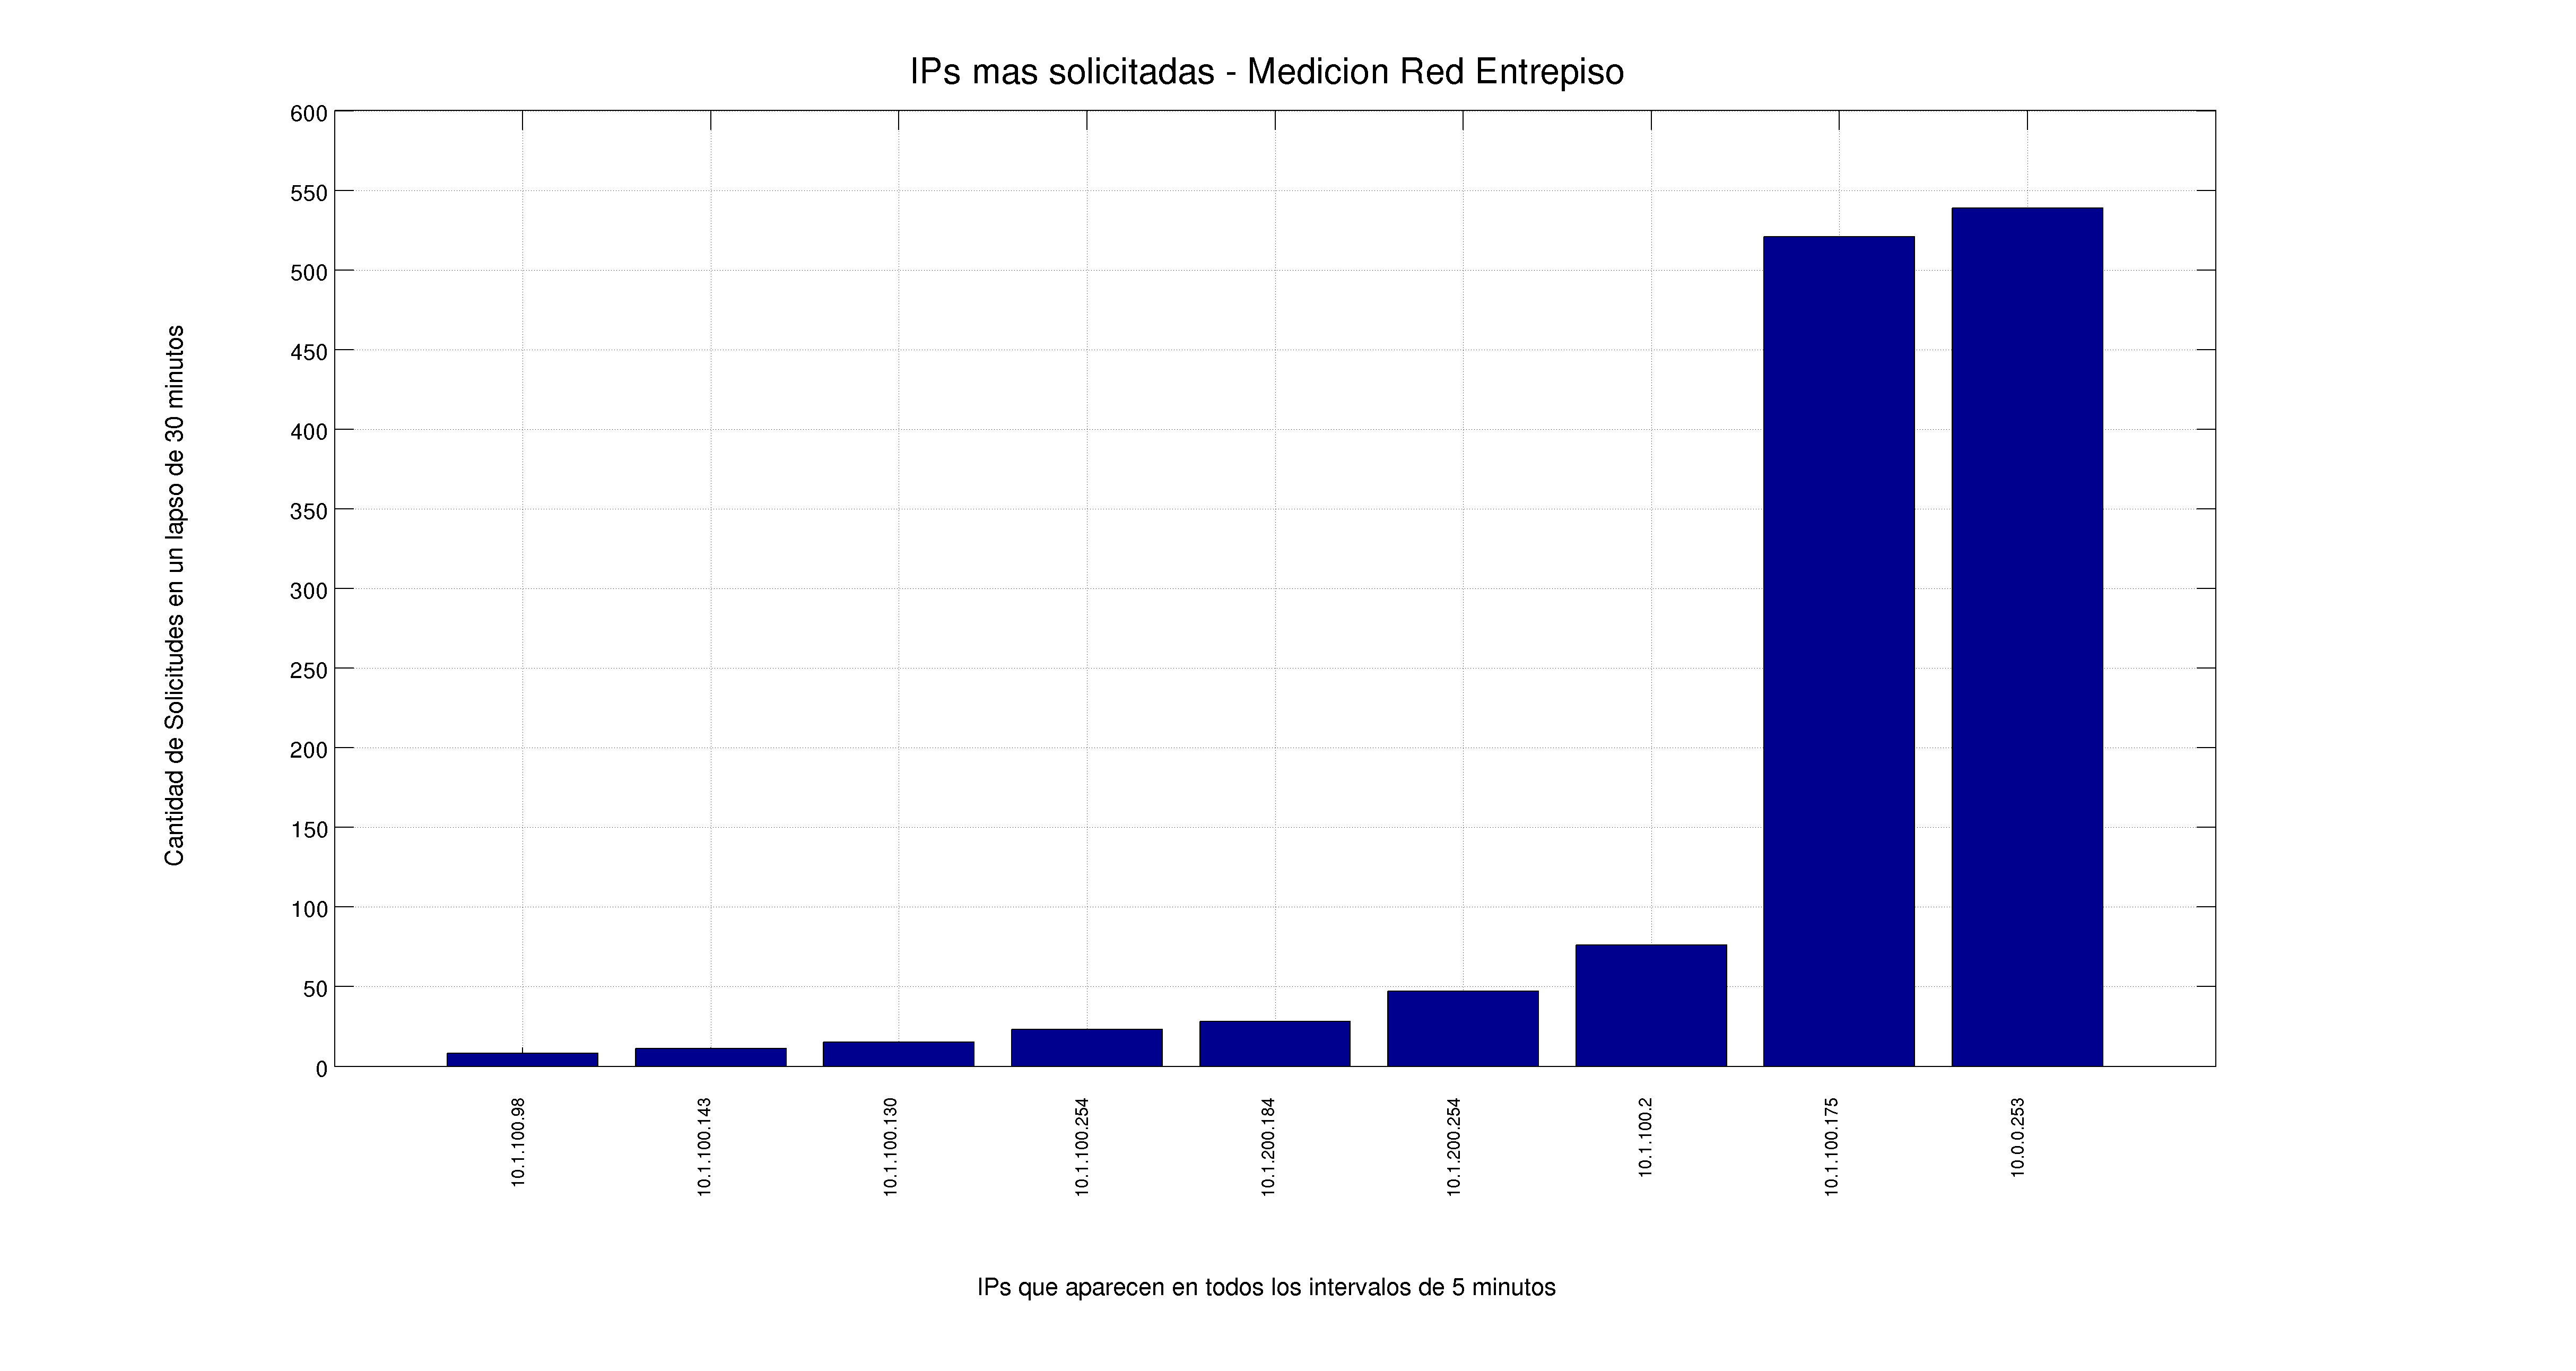
\includegraphics[width=\textwidth, trim=0 0 0 0]{../Graficos/ips_solicitadas_RedEntrepiso_5.png}
\caption{IPs más solicitadas - Red Entrepiso - Intervalos de 15 minutos y de 5 minutos. Las IPs mostradas son las que recibieron {\tt who-has} en todos los
intervalos de tiempo de dicha longitud, de la medición de 30 minutos. Una \emph{solicitud} corresponde a un paquete {\tt who-has} donde la IP aparecía
en el campo ARP\_IP\_DST.} \label{solicitadas-redentrepiso}
\end{figure}

\newpage

\begin{figure}[h!]
\centering
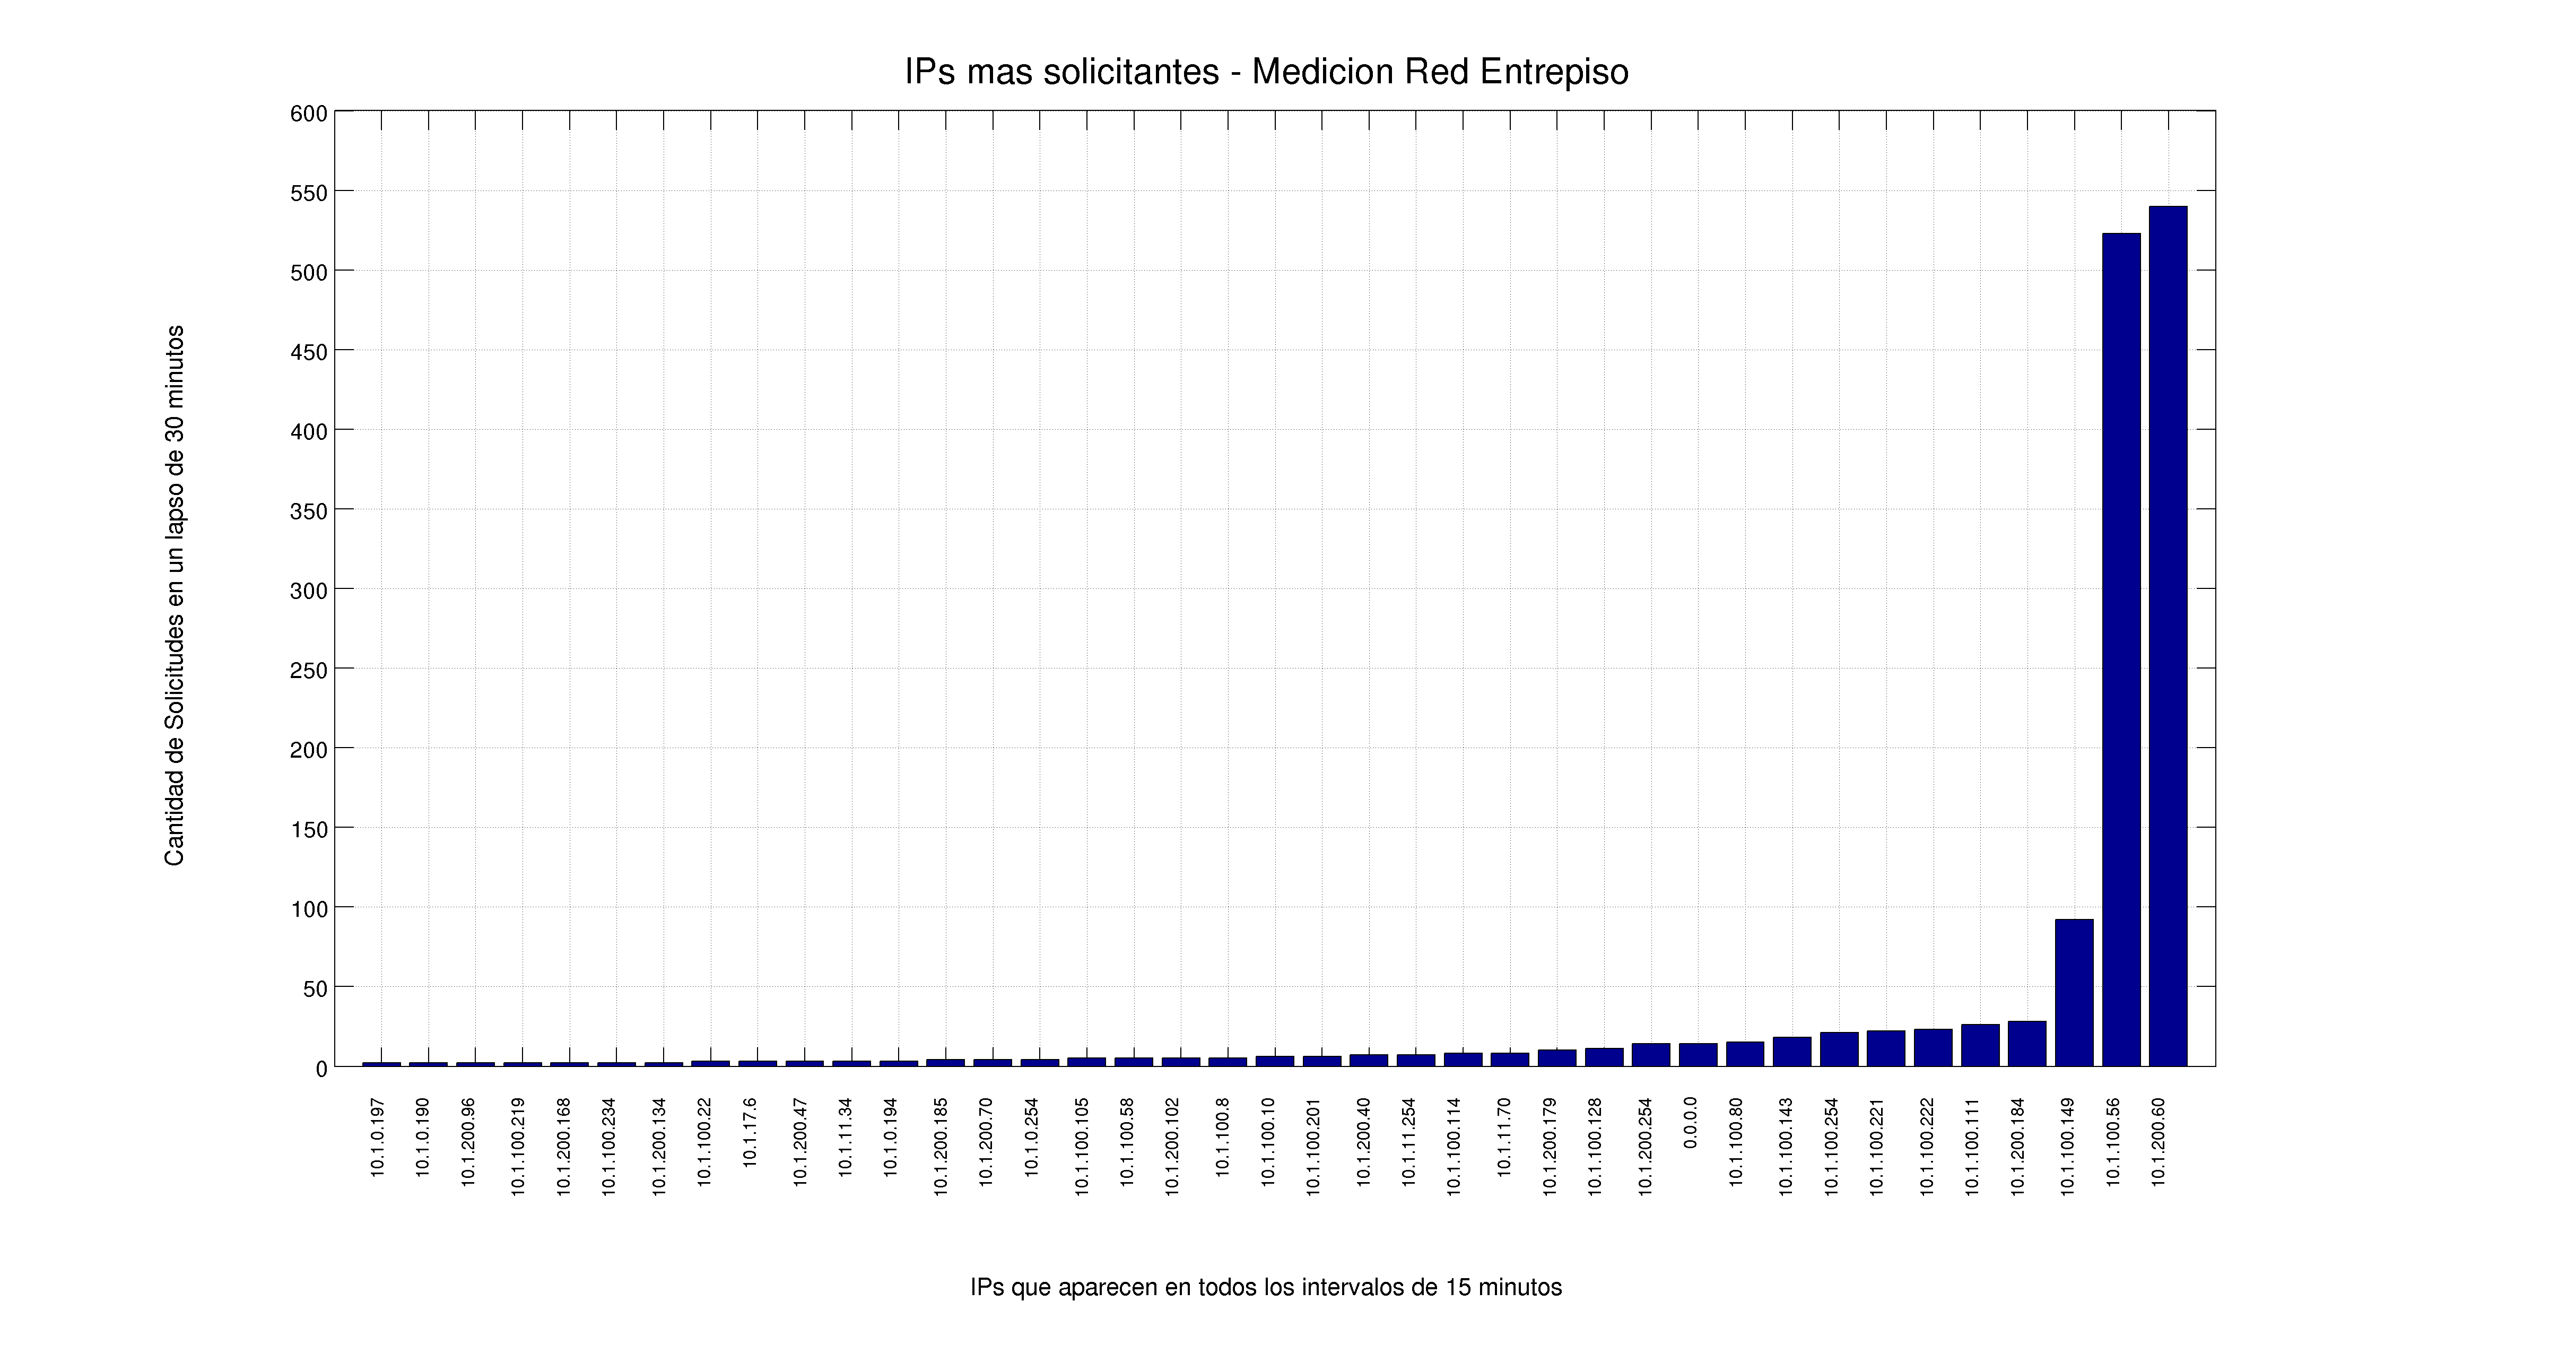
\includegraphics[width=\textwidth, trim=0 0 0 0]{../Graficos/ips_solicitantes_RedEntrepiso_15.png}

\caption{IPs más solicitantes - Red Entrepiso - Intervalos de 15 minutos. Las IPs mostradas son las que enviaron {\tt who-has} en todos los
intervalos de tiempo de dicha longitud, de la medición de 30 minutos. Una \emph{solicitud} corresponde a un paquete {\tt who-has} donde la IP aparecía
en el campo ARP\_IP\_SRC.} \label{solicitantes-redentrepiso}
\end{figure}


\begin{figure}[h!]
\centering
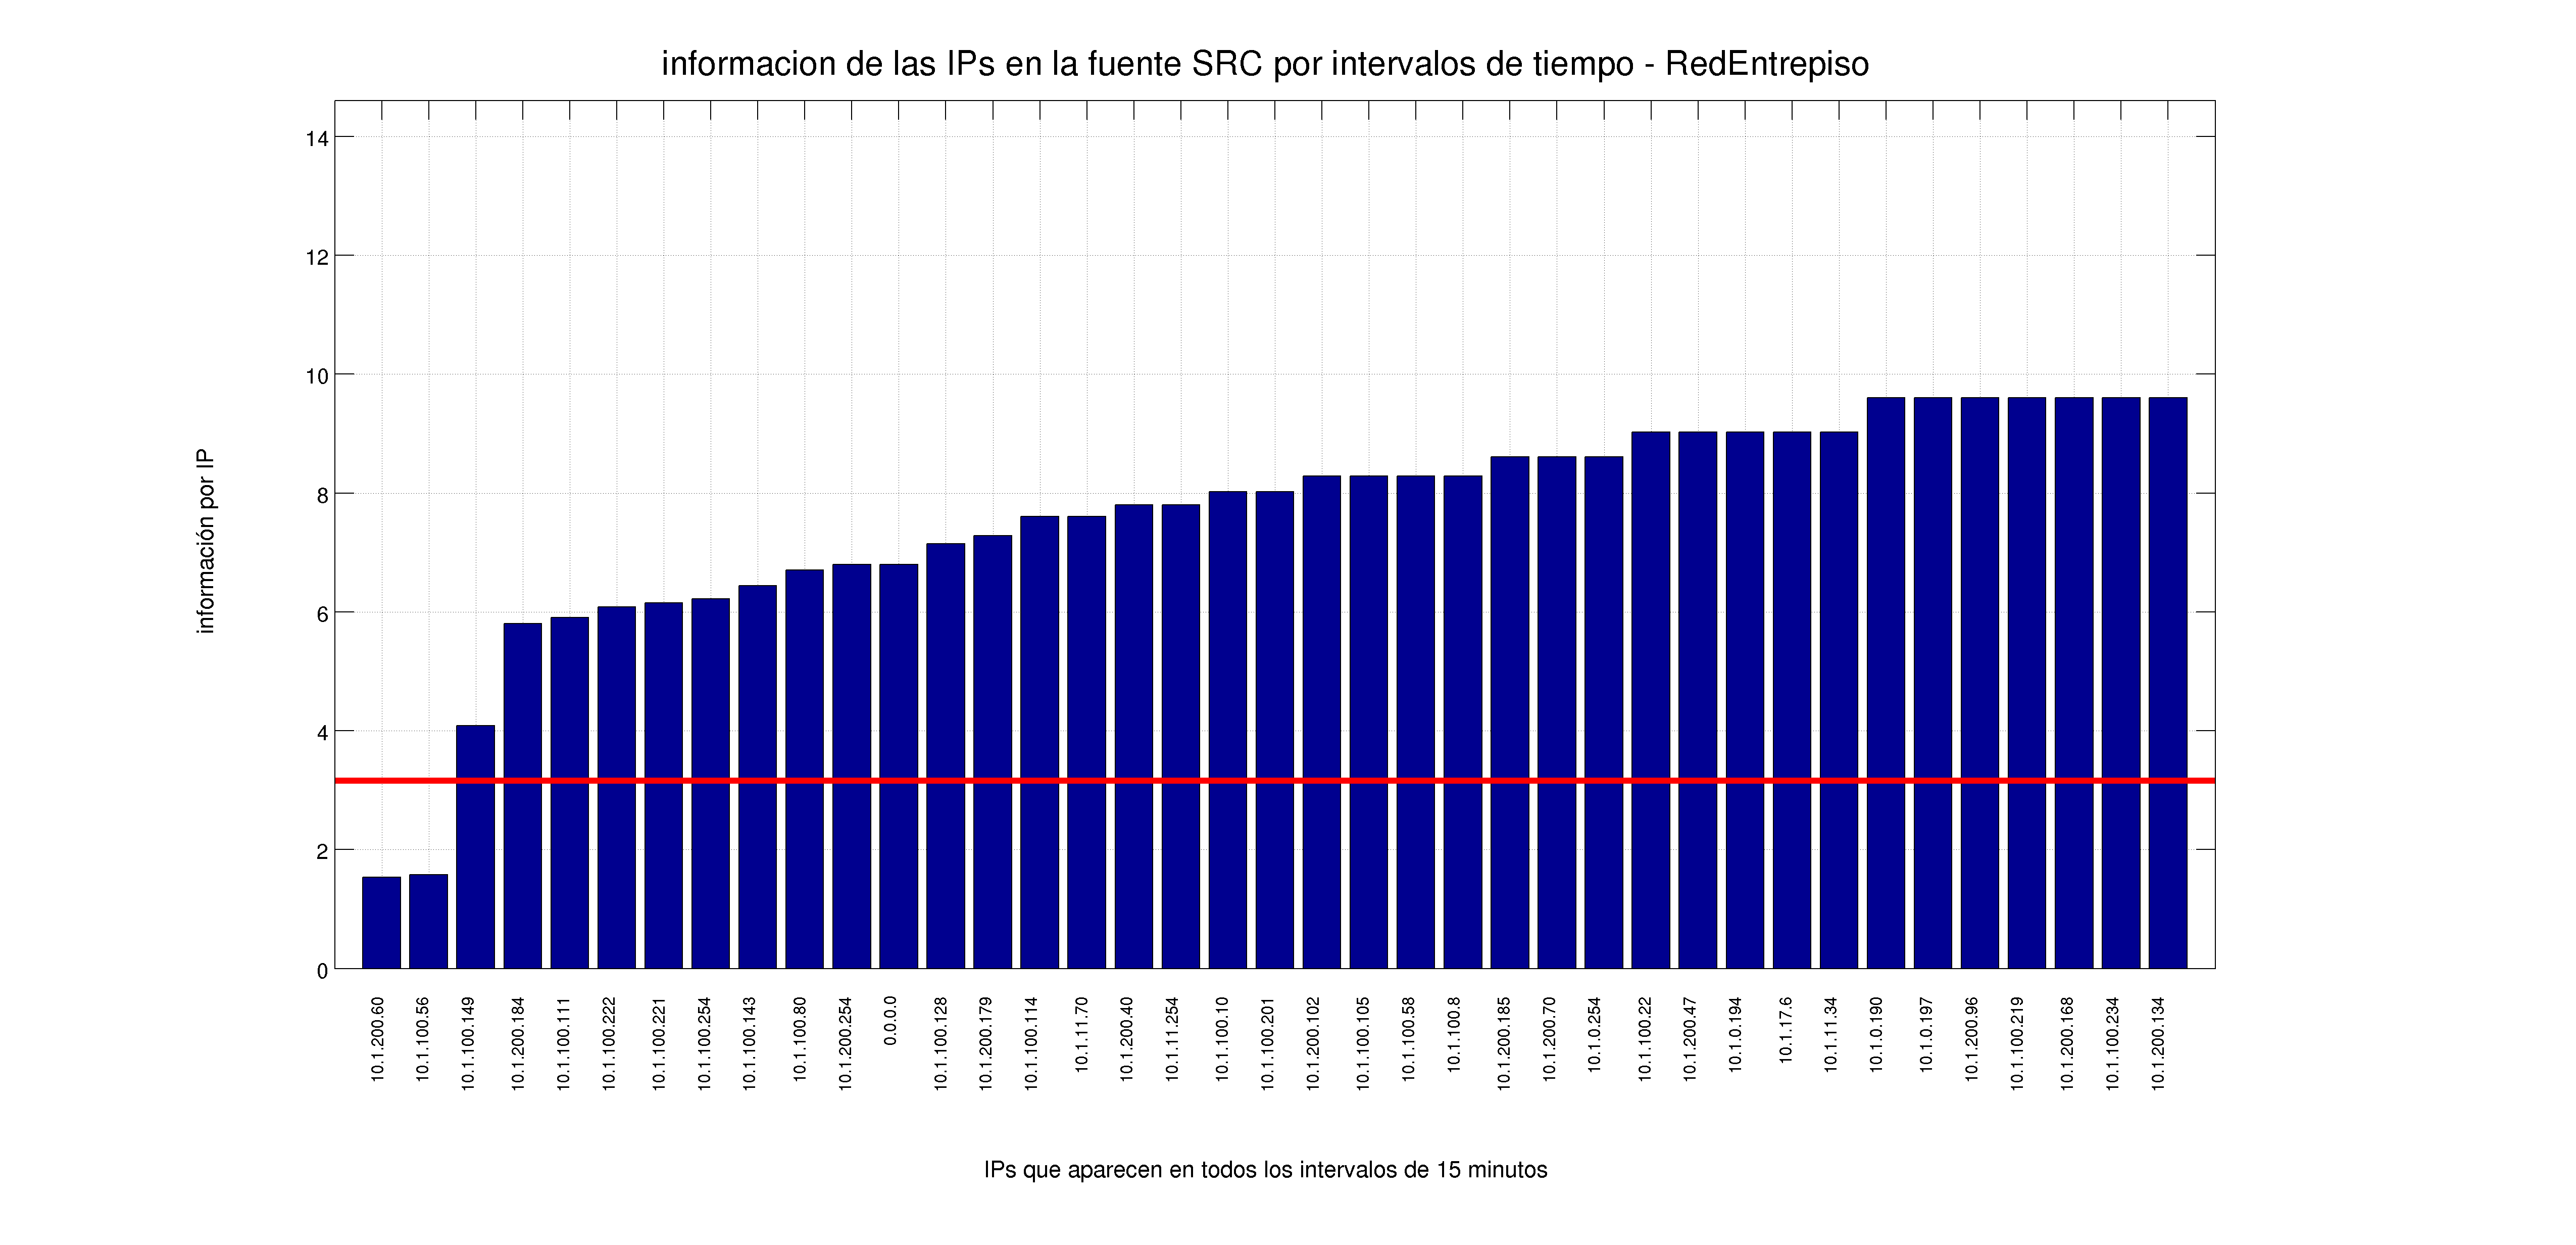
\includegraphics[width=\textwidth, trim=0 0 0 0]{../Graficos/entrepiso_infoConEn_15.png}

\caption{Información y Entropía (rojo) - Fuente $S_{src}$ - Red Entrepiso - Intervalos de 15 minutos. Las IPs mostradas son las que enviaron {\tt who-has} en todos los
intervalos de tiempo de dicha longitud, de la medición de 30 minutos.}
\end{figure}


\newpage

\begin{figure}[h!]
\centering
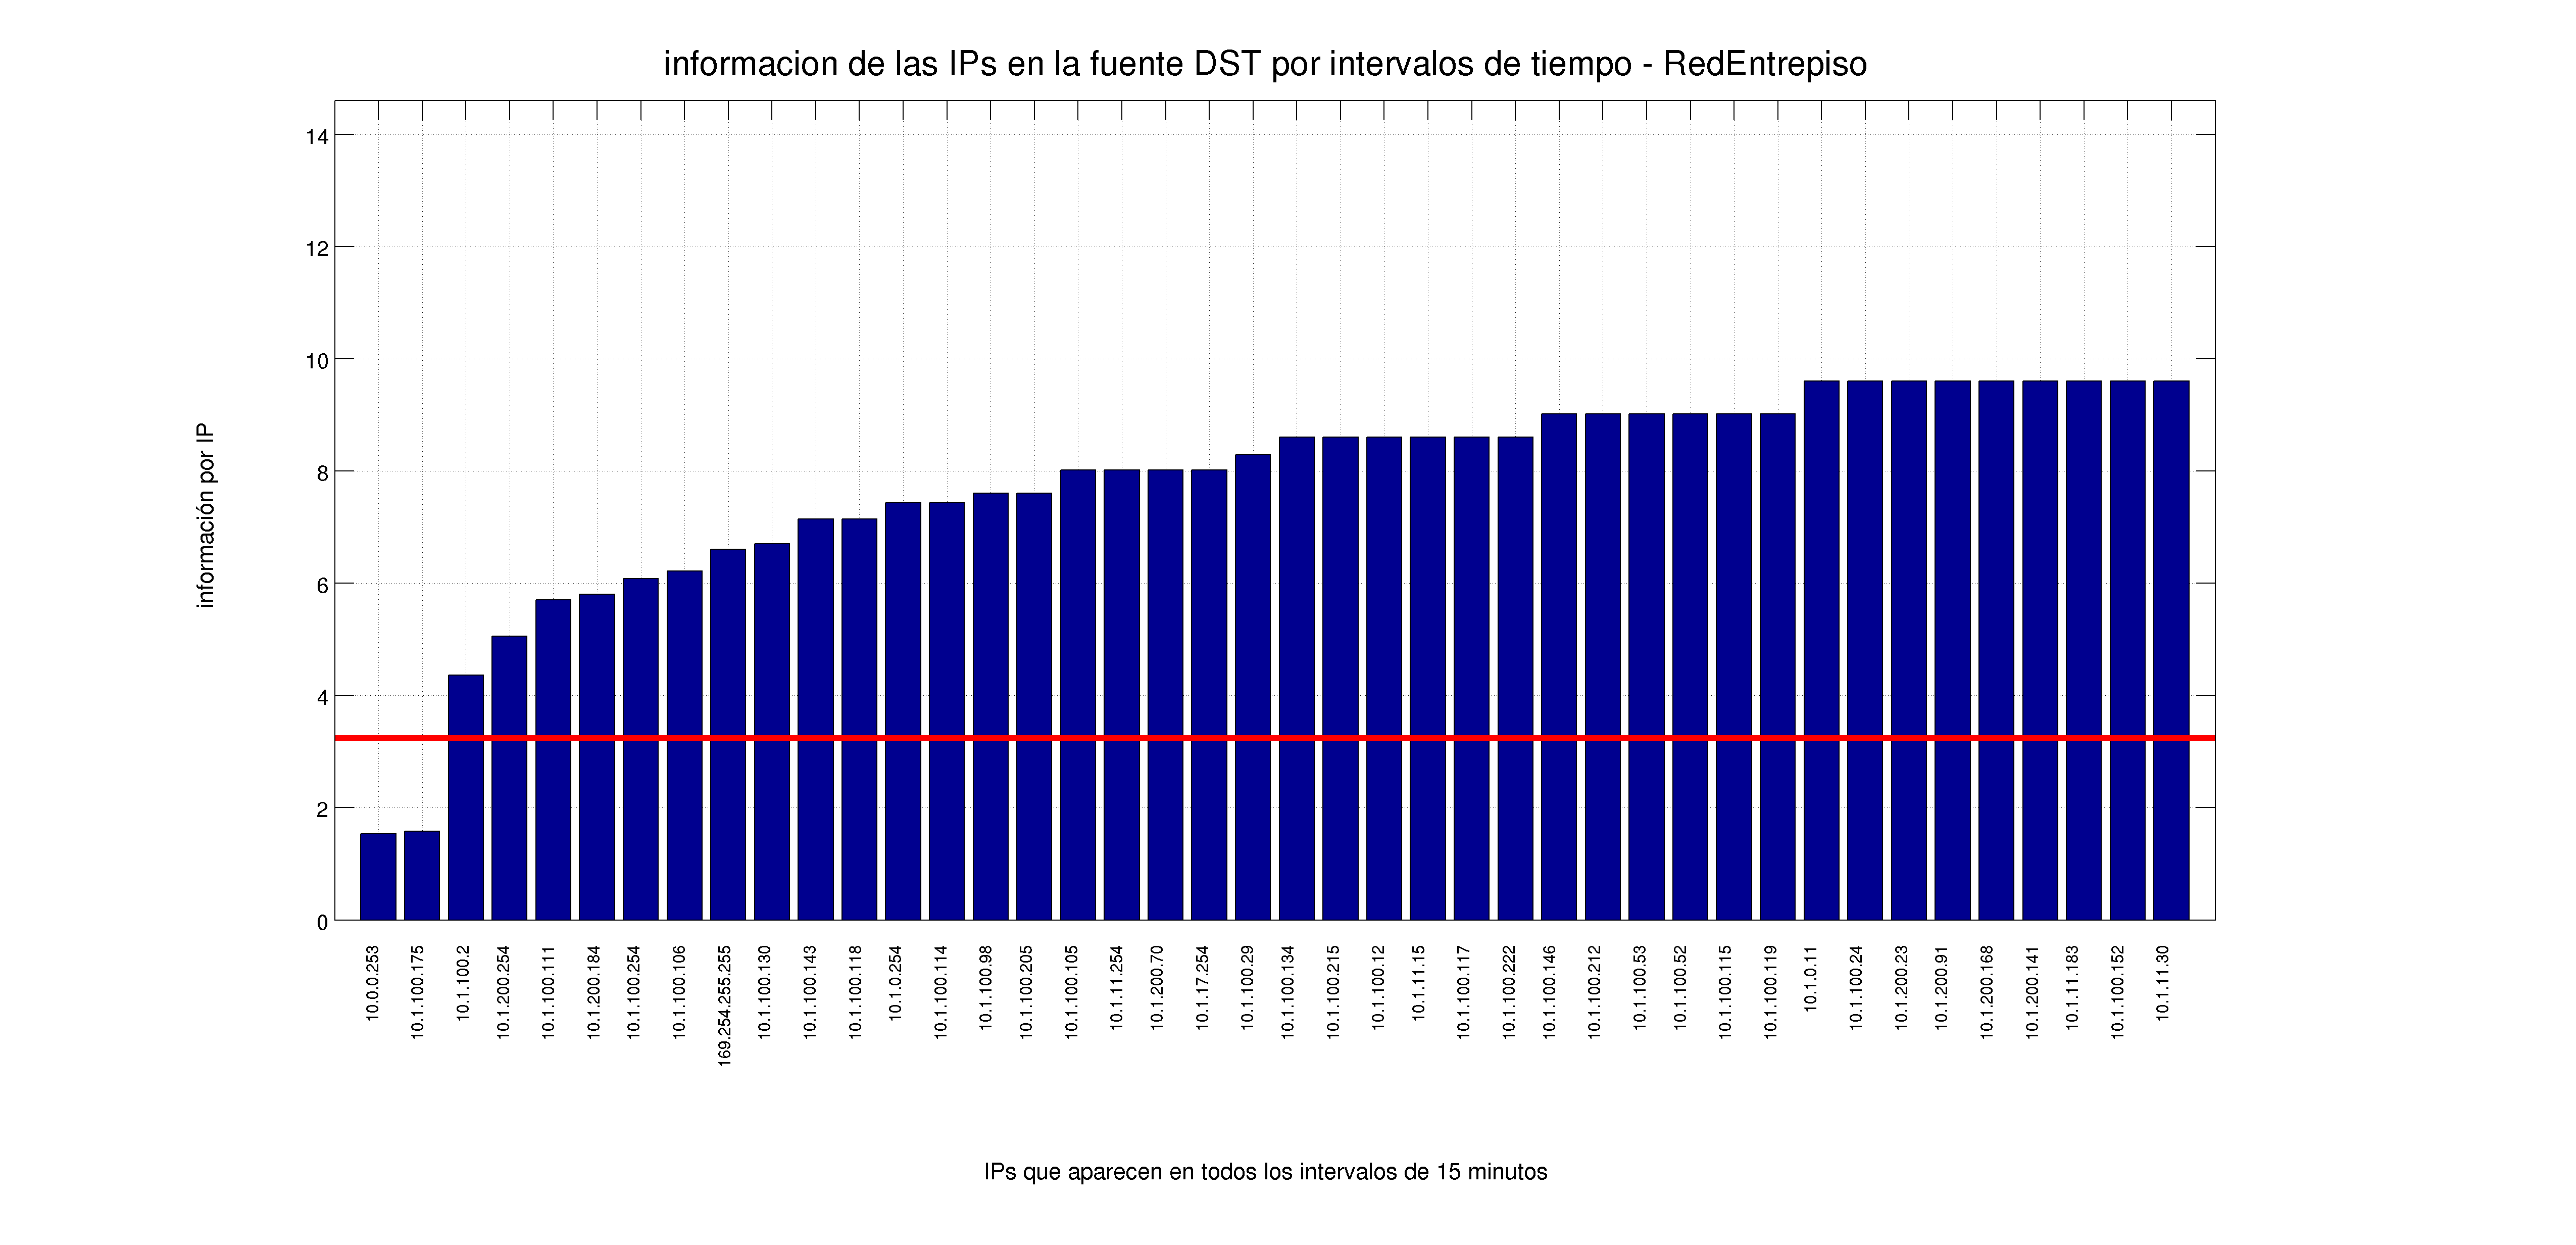
\includegraphics[width=\textwidth, trim=0 0 0 0]{../Graficos/entrepiso_infoConEn_dst_15.png}

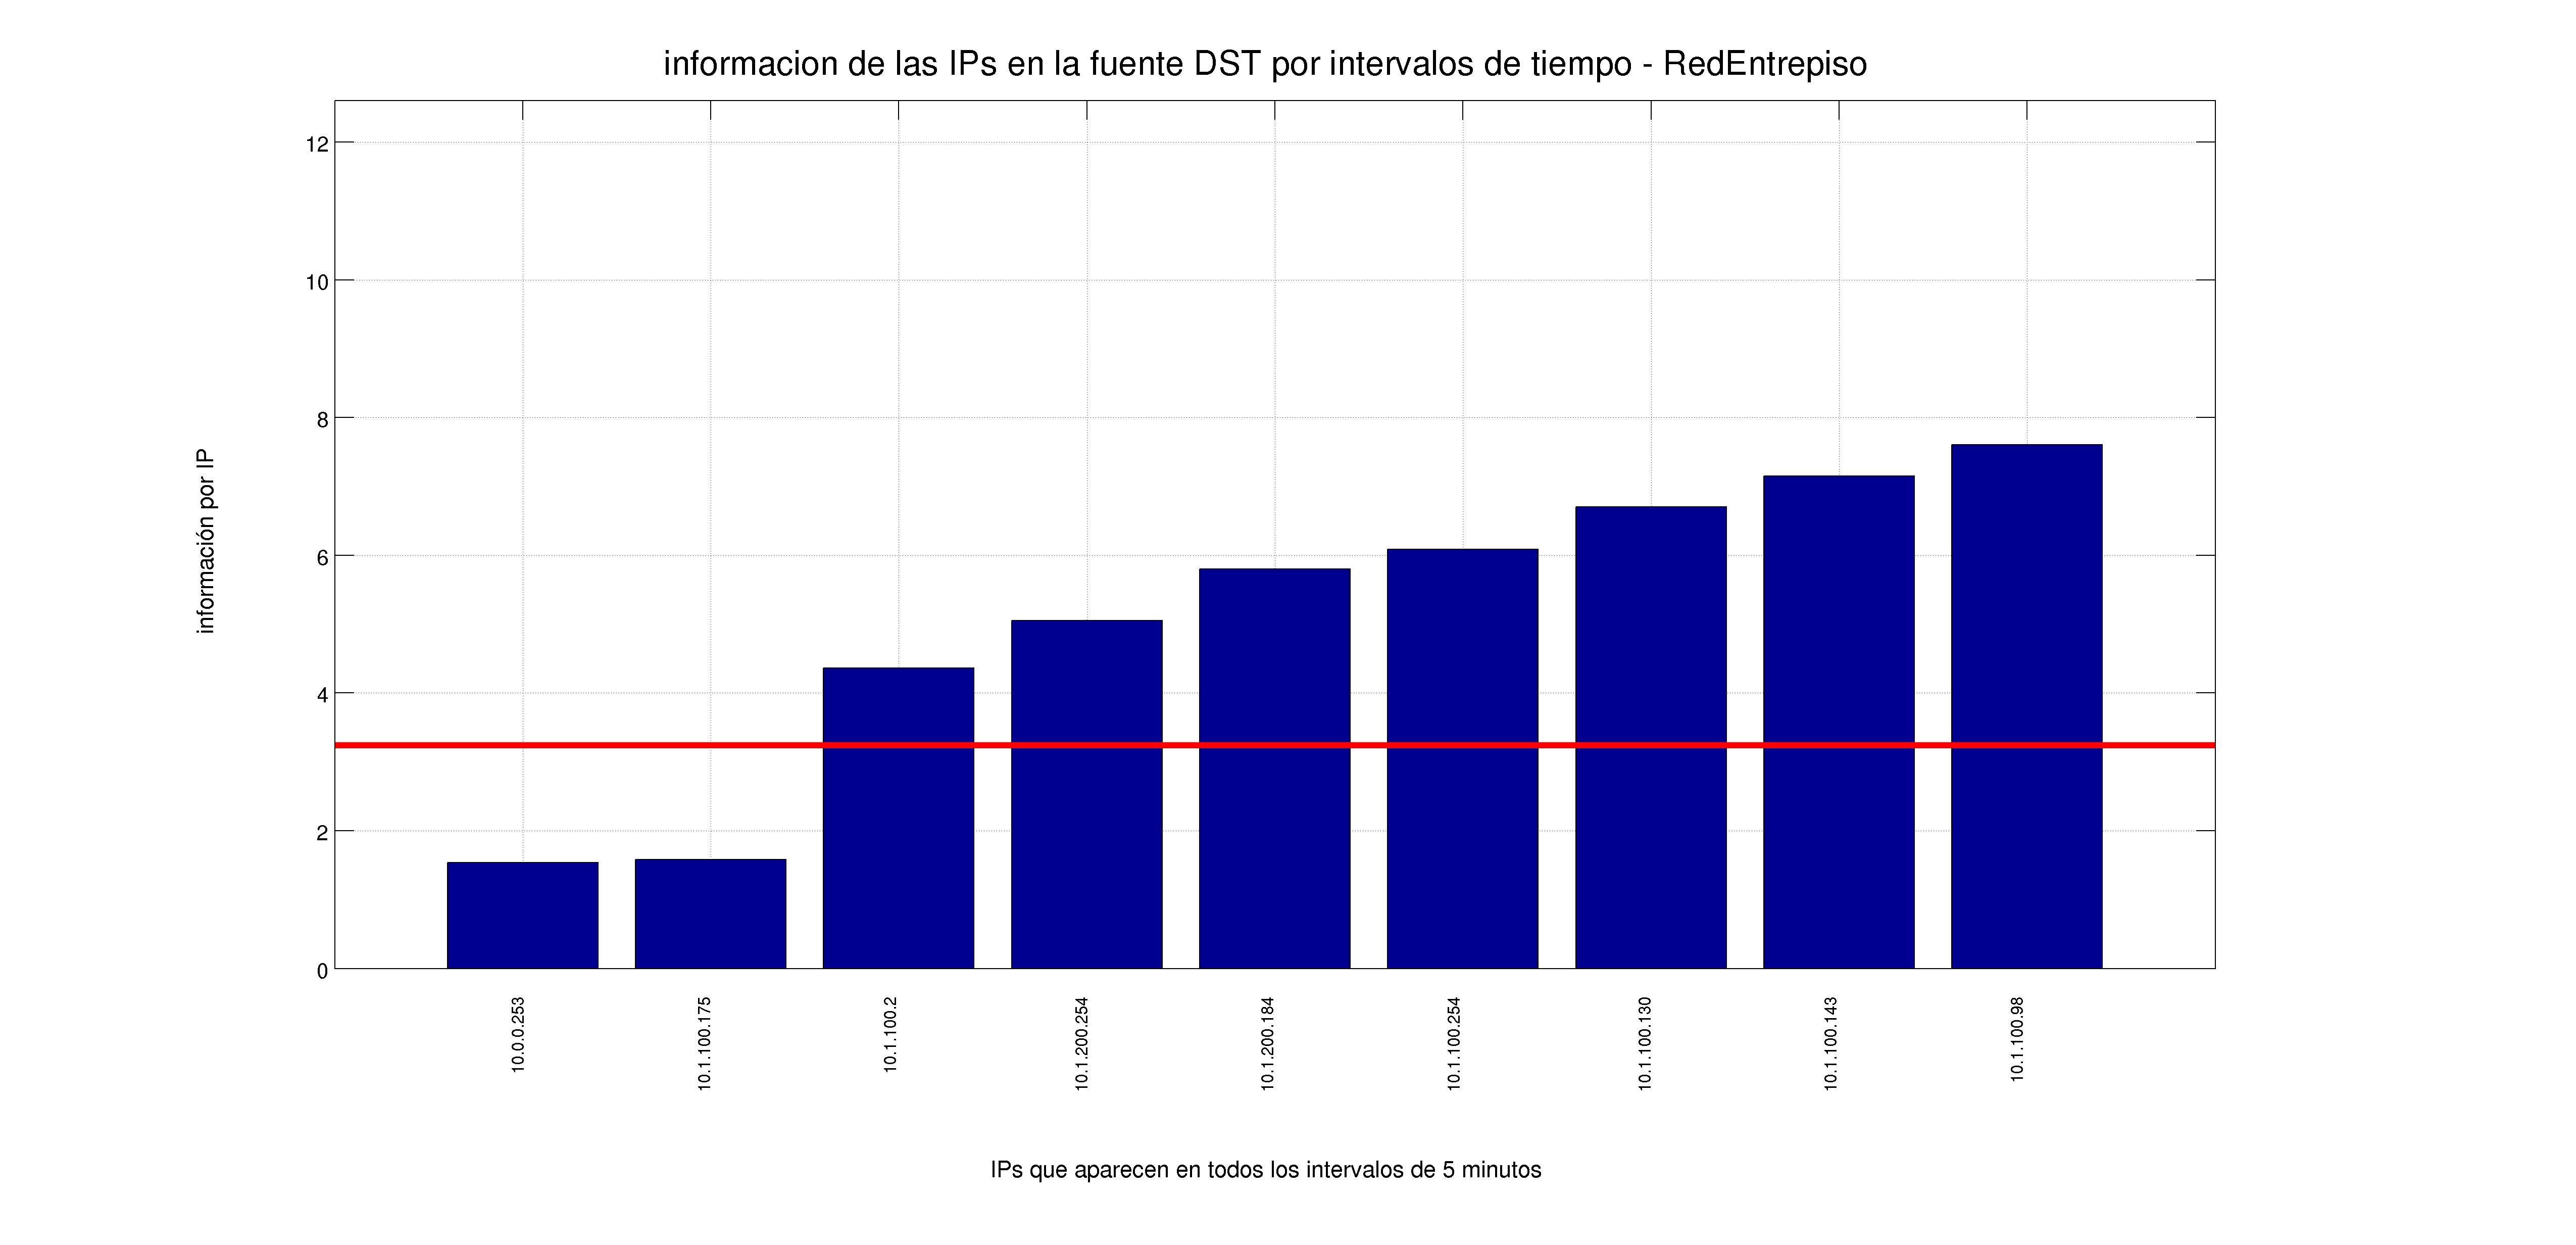
\includegraphics[width=\textwidth, trim=0 0 0 0]{../Graficos/entrepiso_infoConEn_dst_5.png}
\caption{Información y Entropía (rojo) - Fuente $S_{dst}$ - Red Entrepiso - Intervalos de 15 minutos y de 5 minutos. Las IPs mostradas son las que enviaron {\tt who-has} en todos los
intervalos de tiempo de dicha longitud, de la medición de 30 minutos.}
\end{figure}

\newpage

\subsection{Red Centro de Estudiantes}

\begin{figure}[h!]
\centering
\includegraphics[width=\textwidth, trim=0 0 0 0]{../Graficos/grafo_CECEN.pdf}
\caption{Envío de paquetes ARP en RedCECEN, durante media hora de muestreo. Los nodos corresponden a IPs. Los ejes indican un envío de paquete
{\tt who-has} broadcast, relacionando IP fuente con IP destino. El peso de los ejes es la cantidad de paquetes capturados.}
\end{figure}

\newpage

\begin{figure}[h!]
\centering
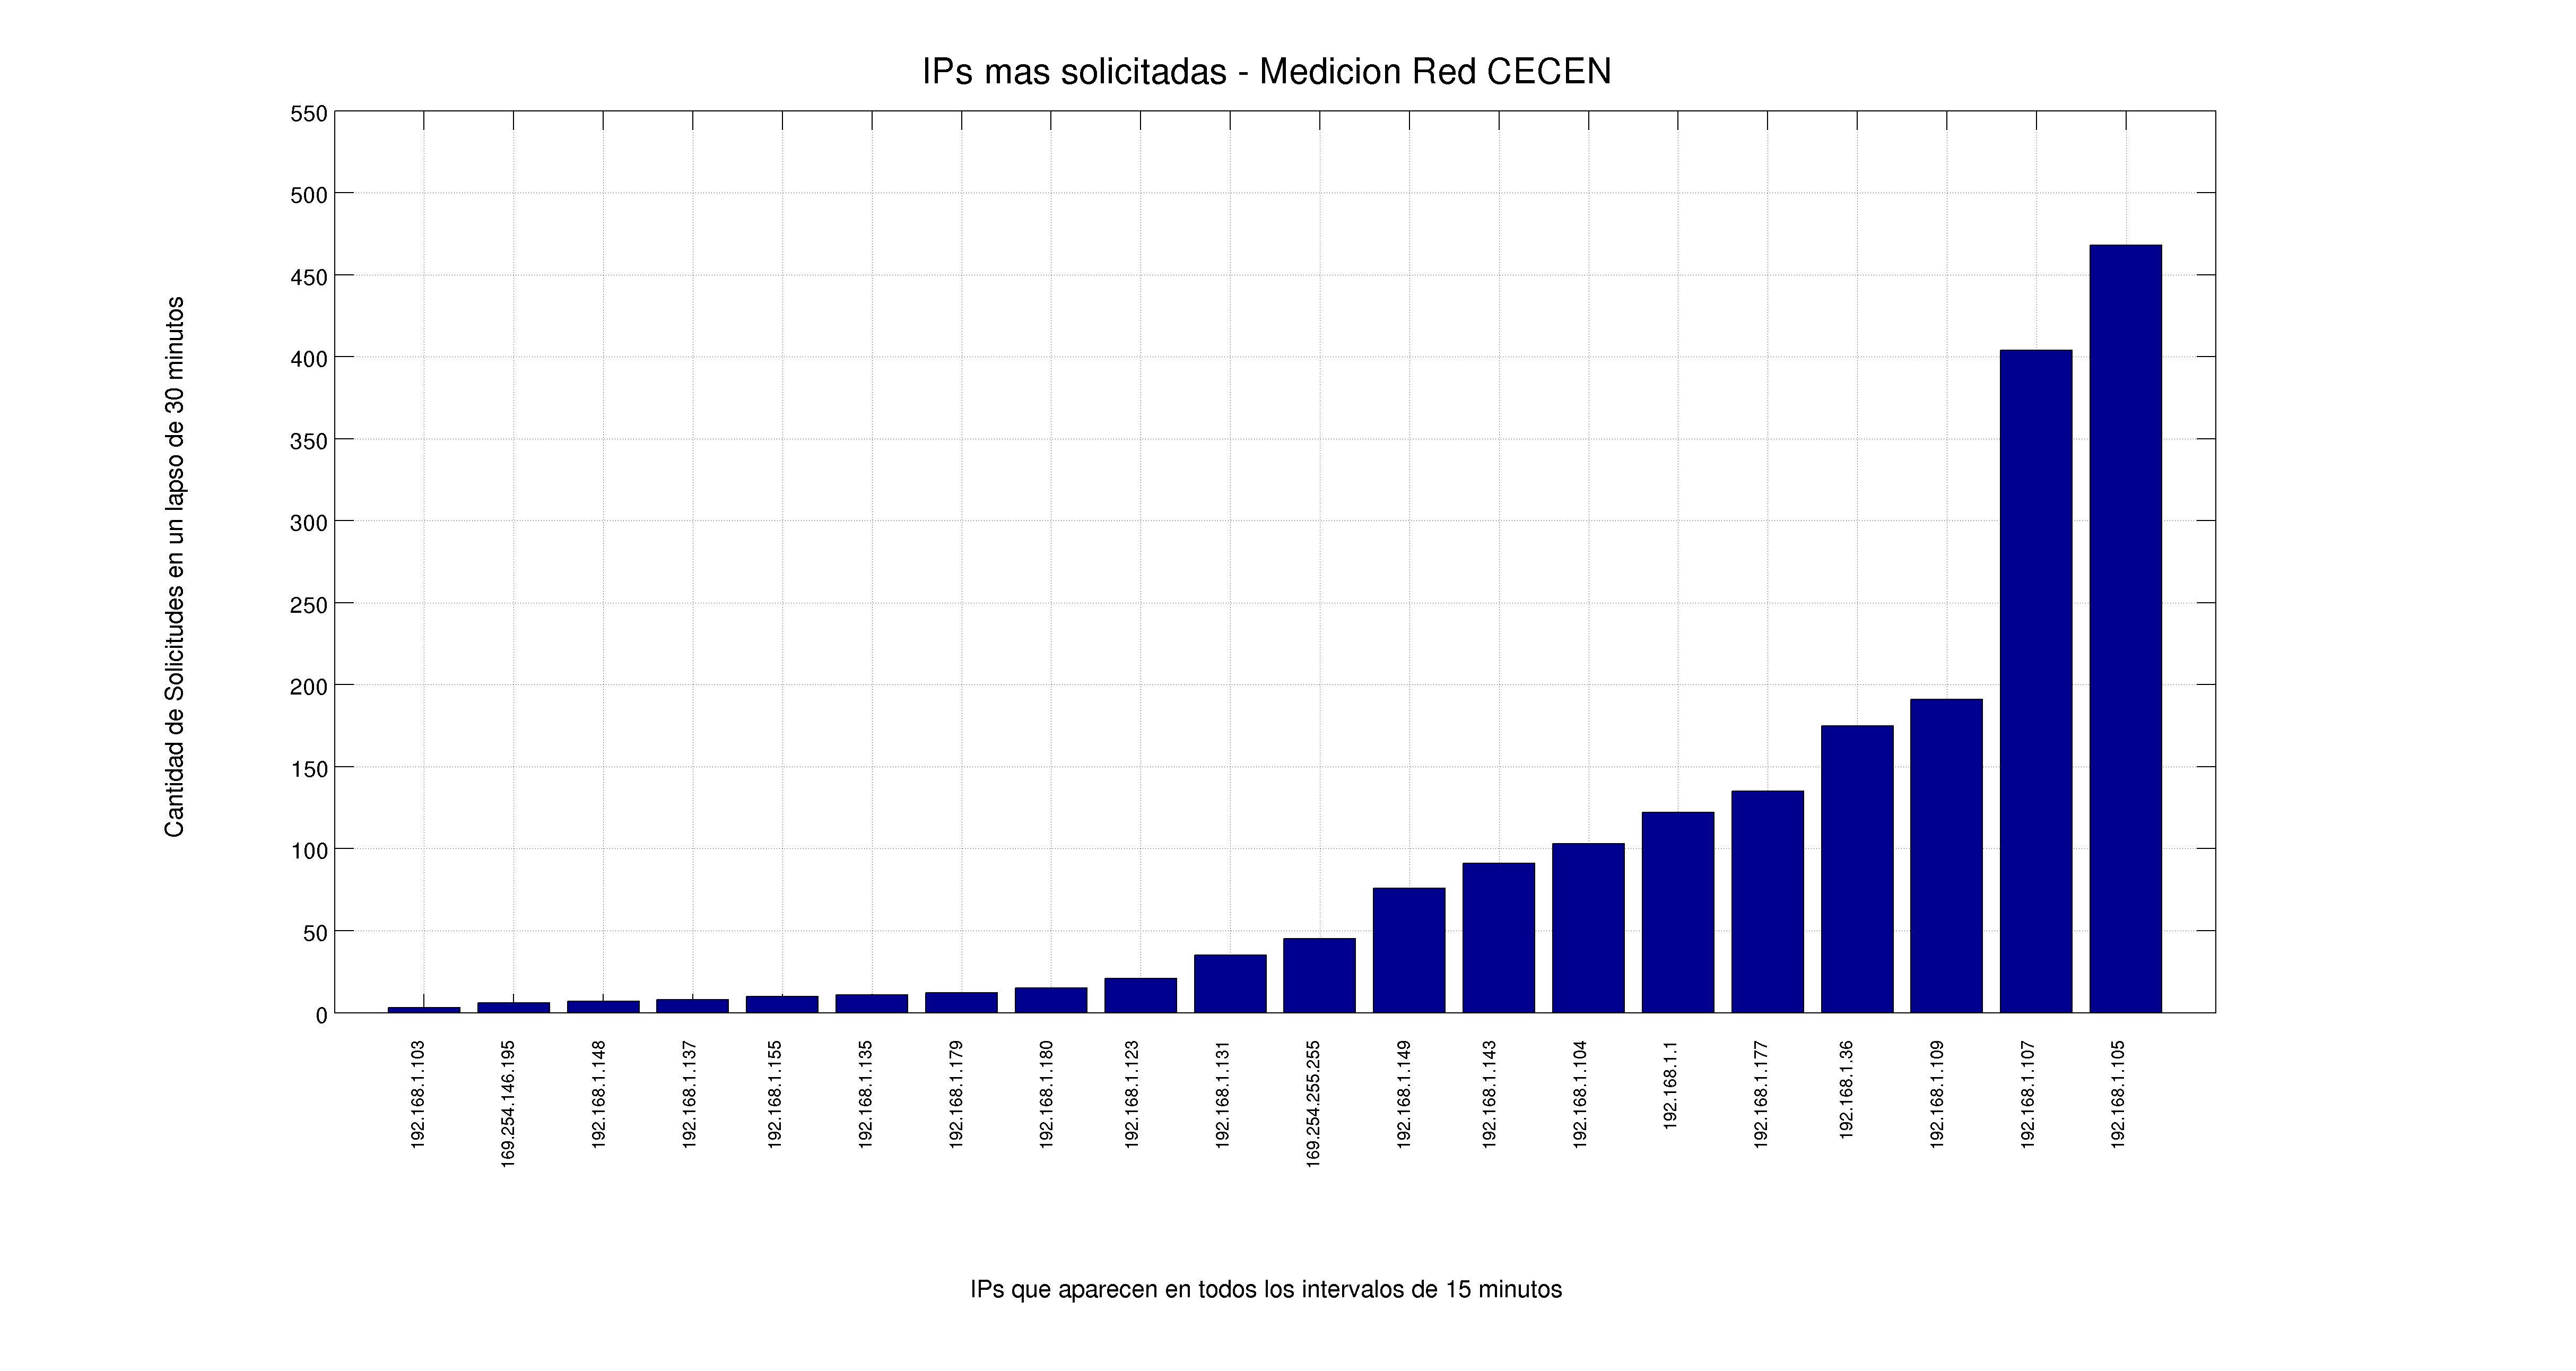
\includegraphics[width=\textwidth, trim=0 0 0 0]{../Graficos/ips_solicitadas_RedCECEN_15.png}

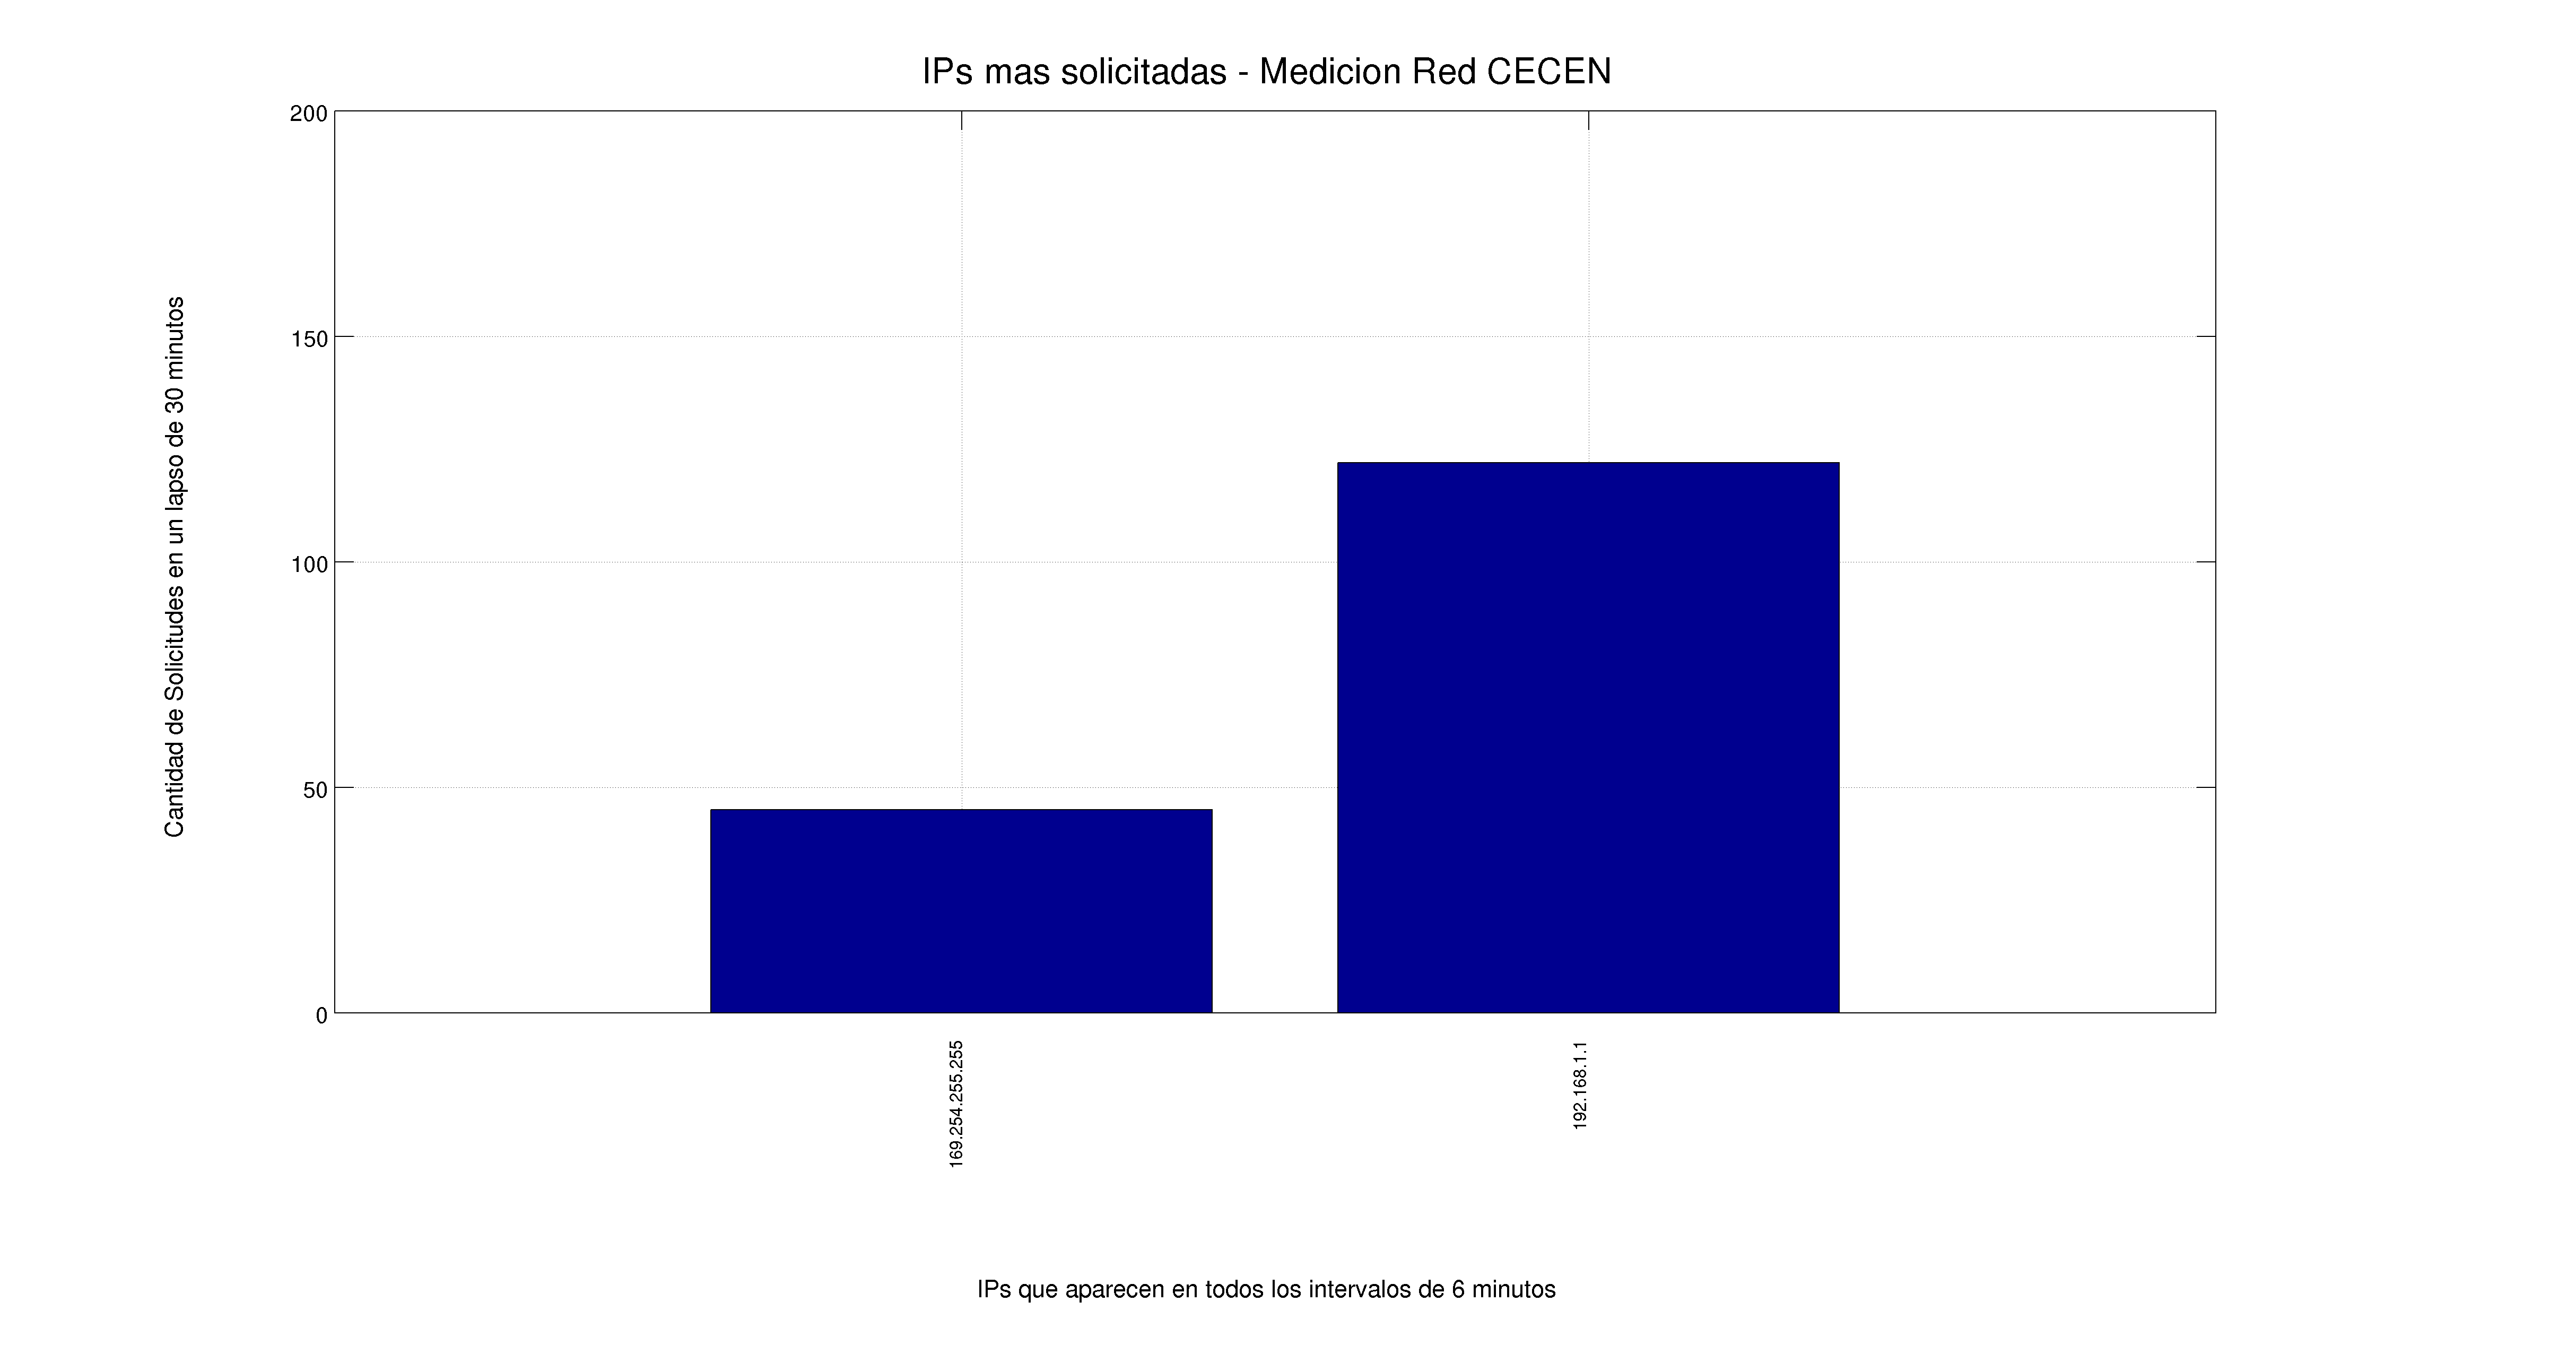
\includegraphics[width=\textwidth, trim=0 0 0 0]{../Graficos/ips_solicitadas_RedCECEN_6.png}
\caption{IPs más solicitadas - Red CECEN - Intervalos de 15 minutos y de 6 minutos. Las IPs mostradas son las que recibieron {\tt who-has} en todos los
intervalos de tiempo de dicha longitud, de la medición de 30 minutos. Una \emph{solicitud} corresponde a un paquete {\tt who-has} donde la IP aparecía
en el campo ARP\_IP\_DST.} \label{solicitadas-redcecen}
\end{figure}

\newpage

\begin{figure}[h!]
\centering
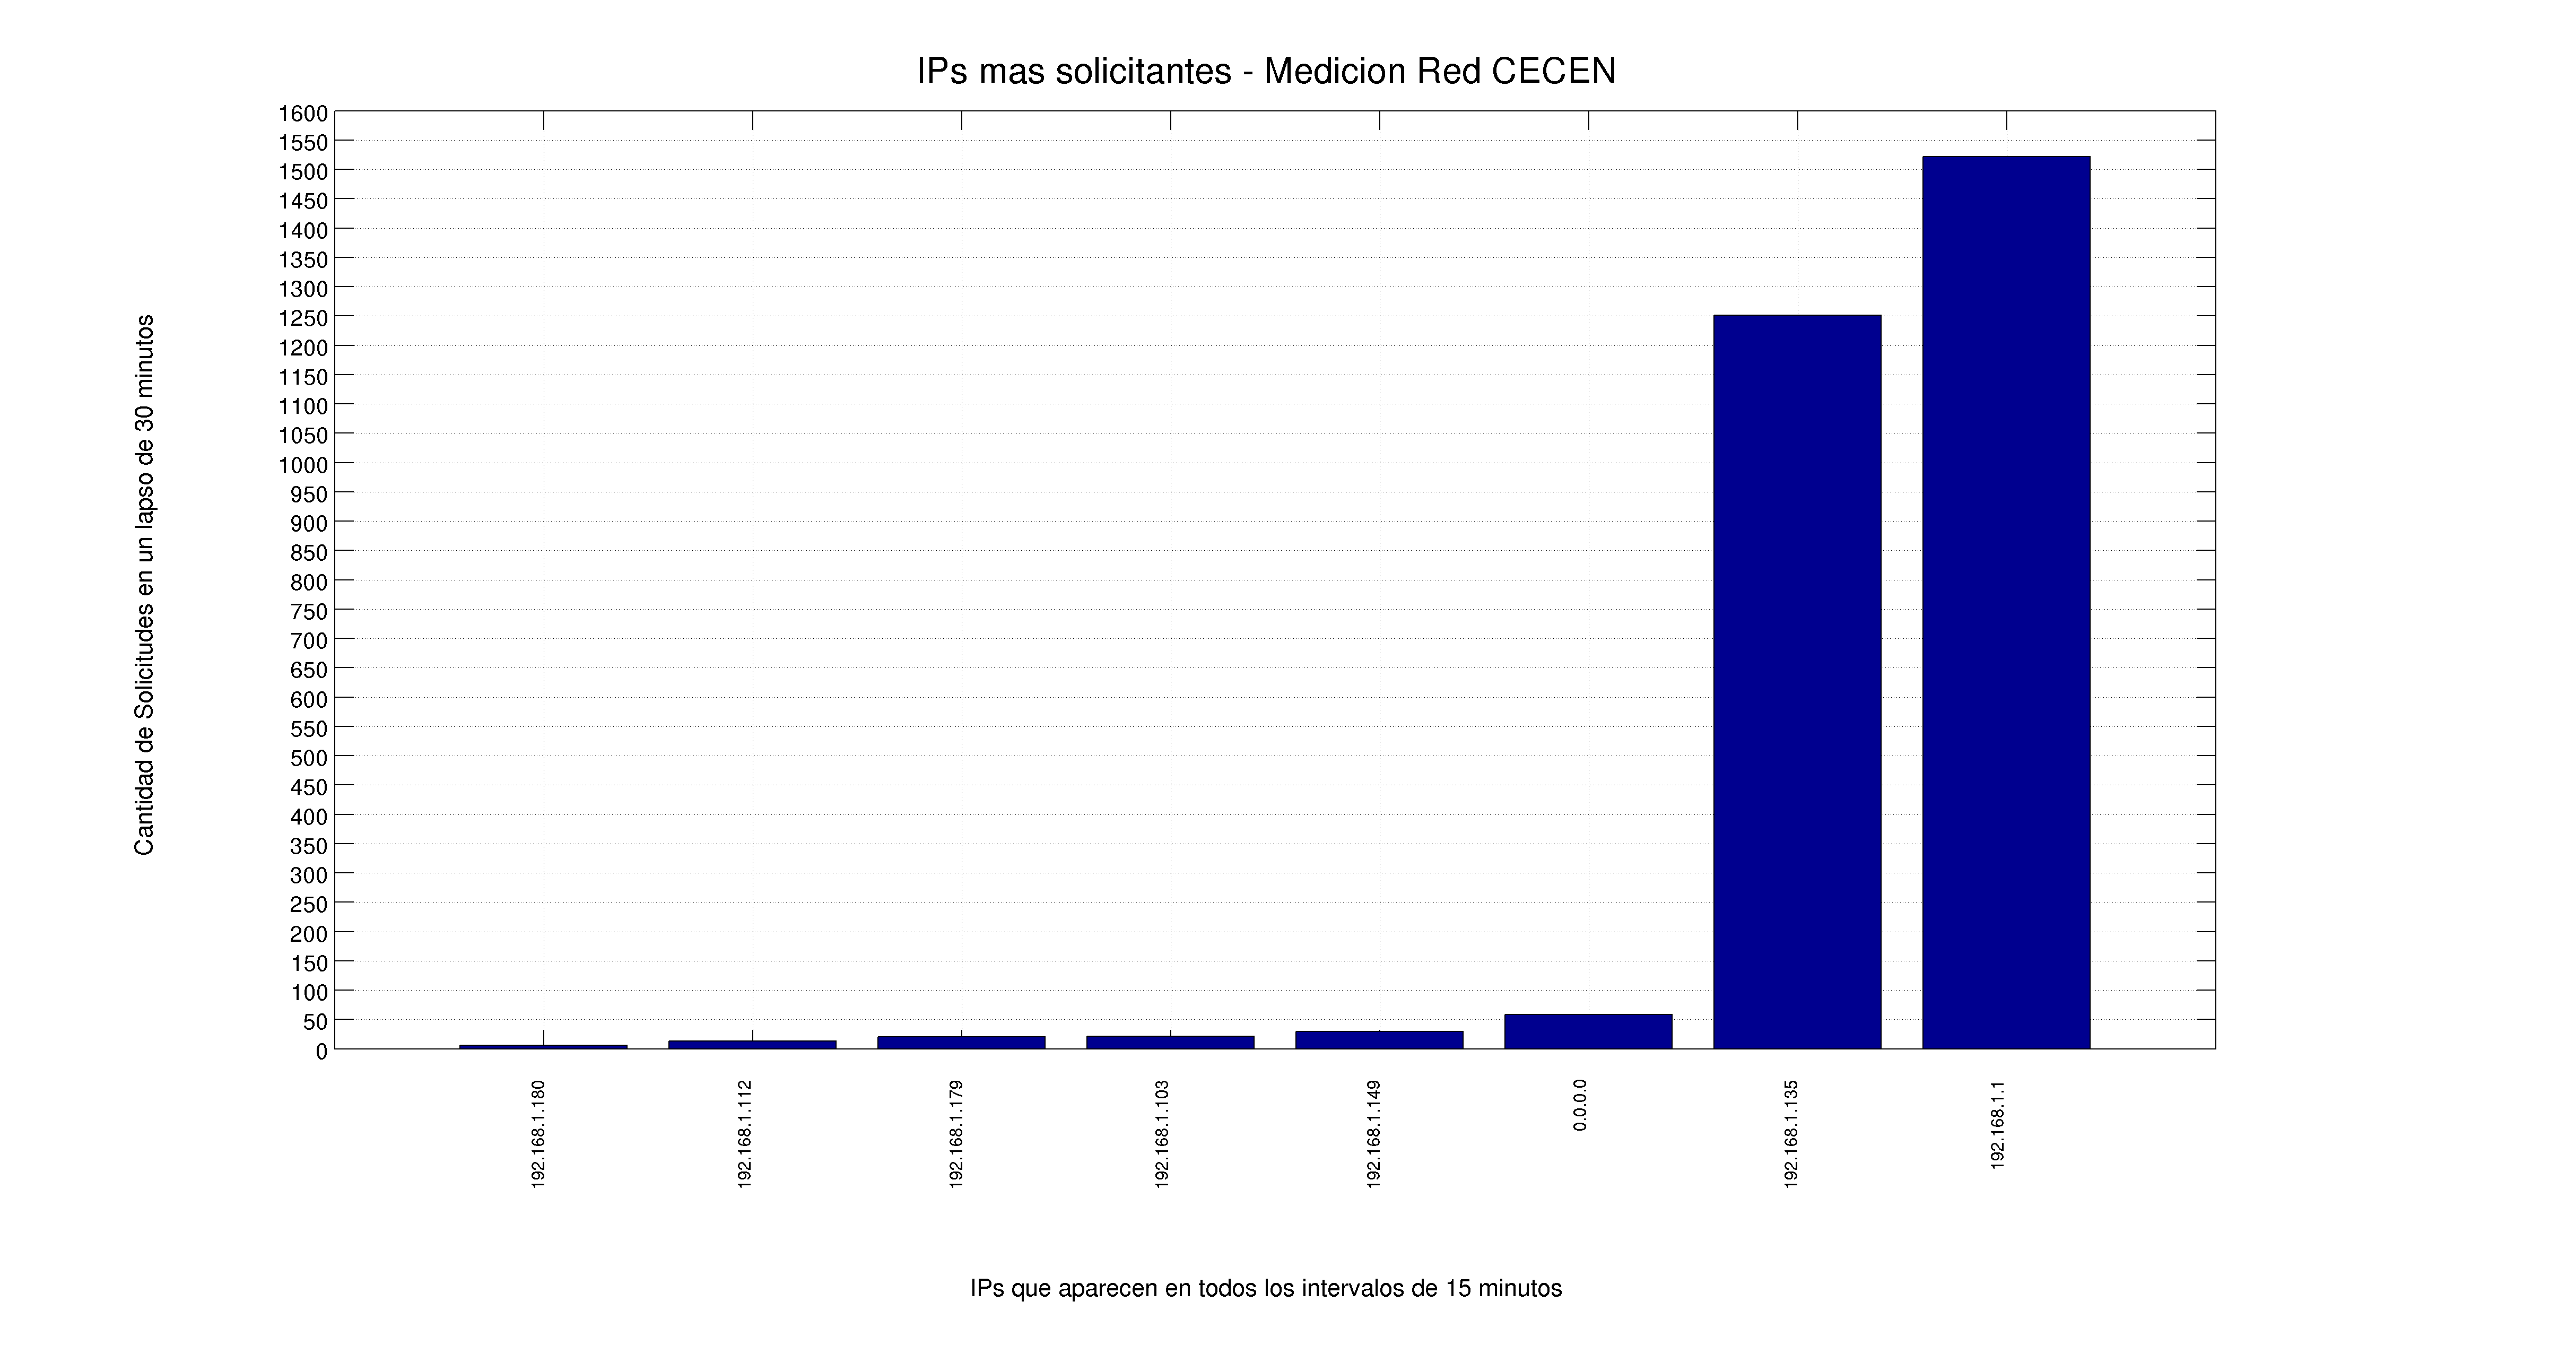
\includegraphics[width=\textwidth, trim=0 0 0 0]{../Graficos/ips_solicitantes_RedCECEN_15.png}

\caption{IPs más solicitantes - Red CECEN - Intervalos de 15 minutos. Las IPs mostradas son las que enviaron {\tt who-has} en todos los
intervalos de tiempo de dicha longitud, de la medición de 30 minutos. Una \emph{solicitud} corresponde a un paquete {\tt who-has} donde la IP aparecía
en el campo ARP\_IP\_SRC.} \label{solicitantes-redcecen}
\end{figure}


\begin{figure}[h!]
\centering
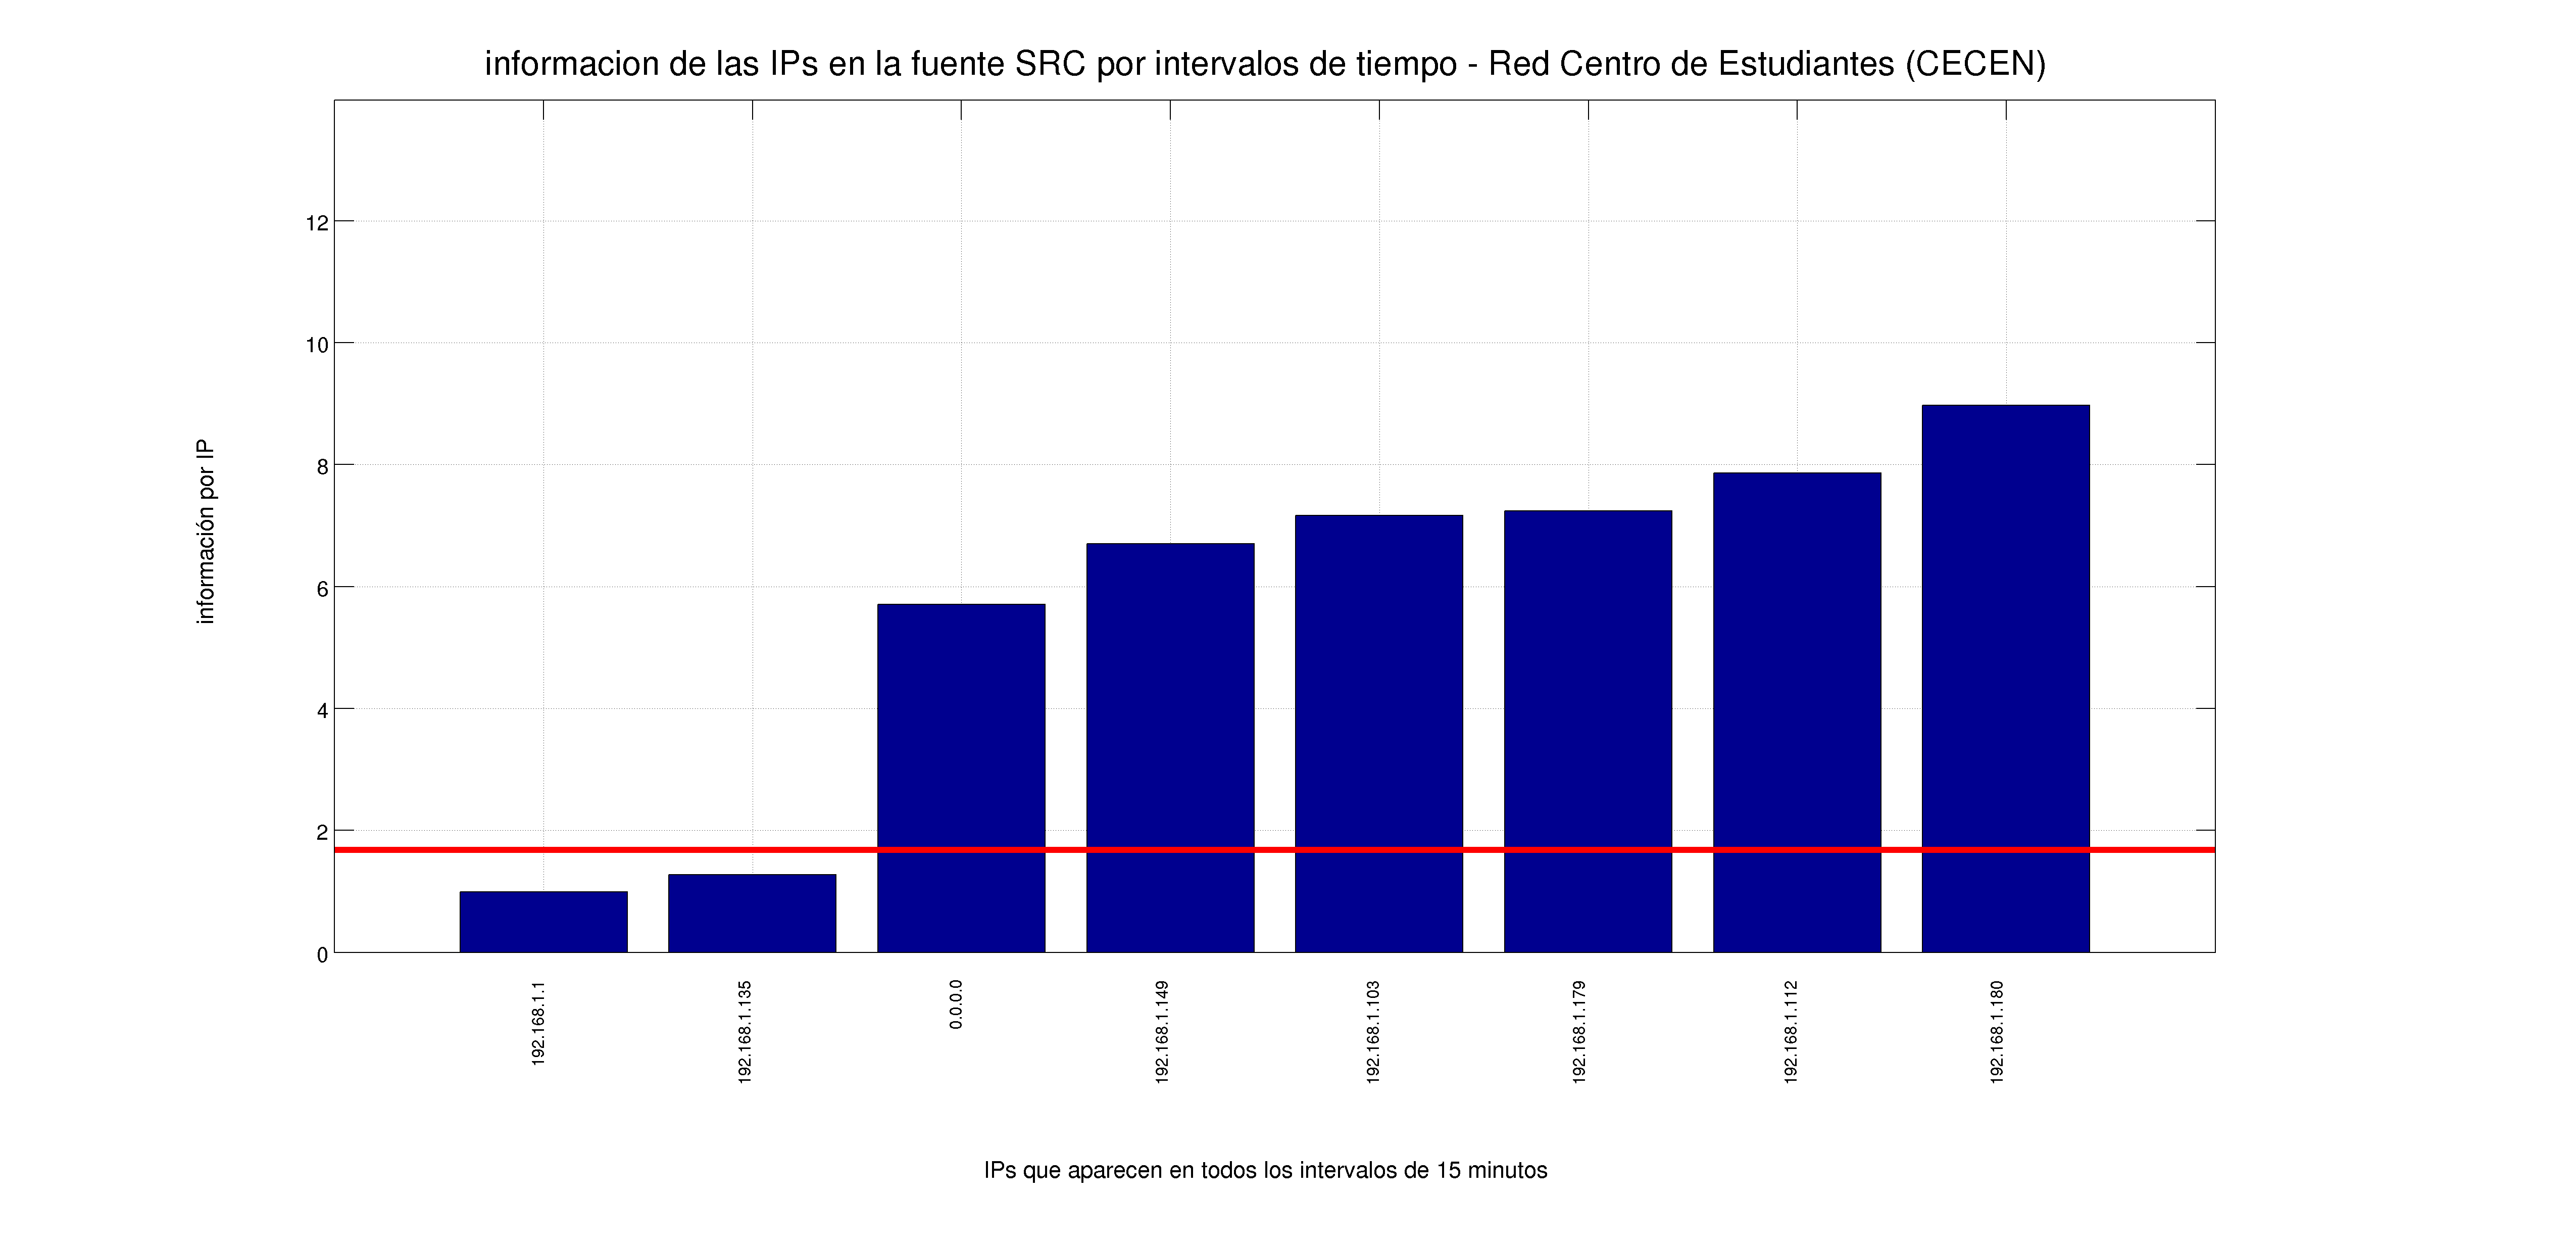
\includegraphics[width=\textwidth, trim=0 0 0 0]{../Graficos/cecen_infoConEn_15.png}

\caption{Información y Entropía (rojo) - Fuente $S_{src}$ - Red CECEN - Intervalos de 15 minutos. Las IPs mostradas son las que enviaron {\tt who-has} en todos los
intervalos de tiempo de dicha longitud, de la medición de 30 minutos.}
\end{figure}


\newpage

\begin{figure}[h!]
\centering
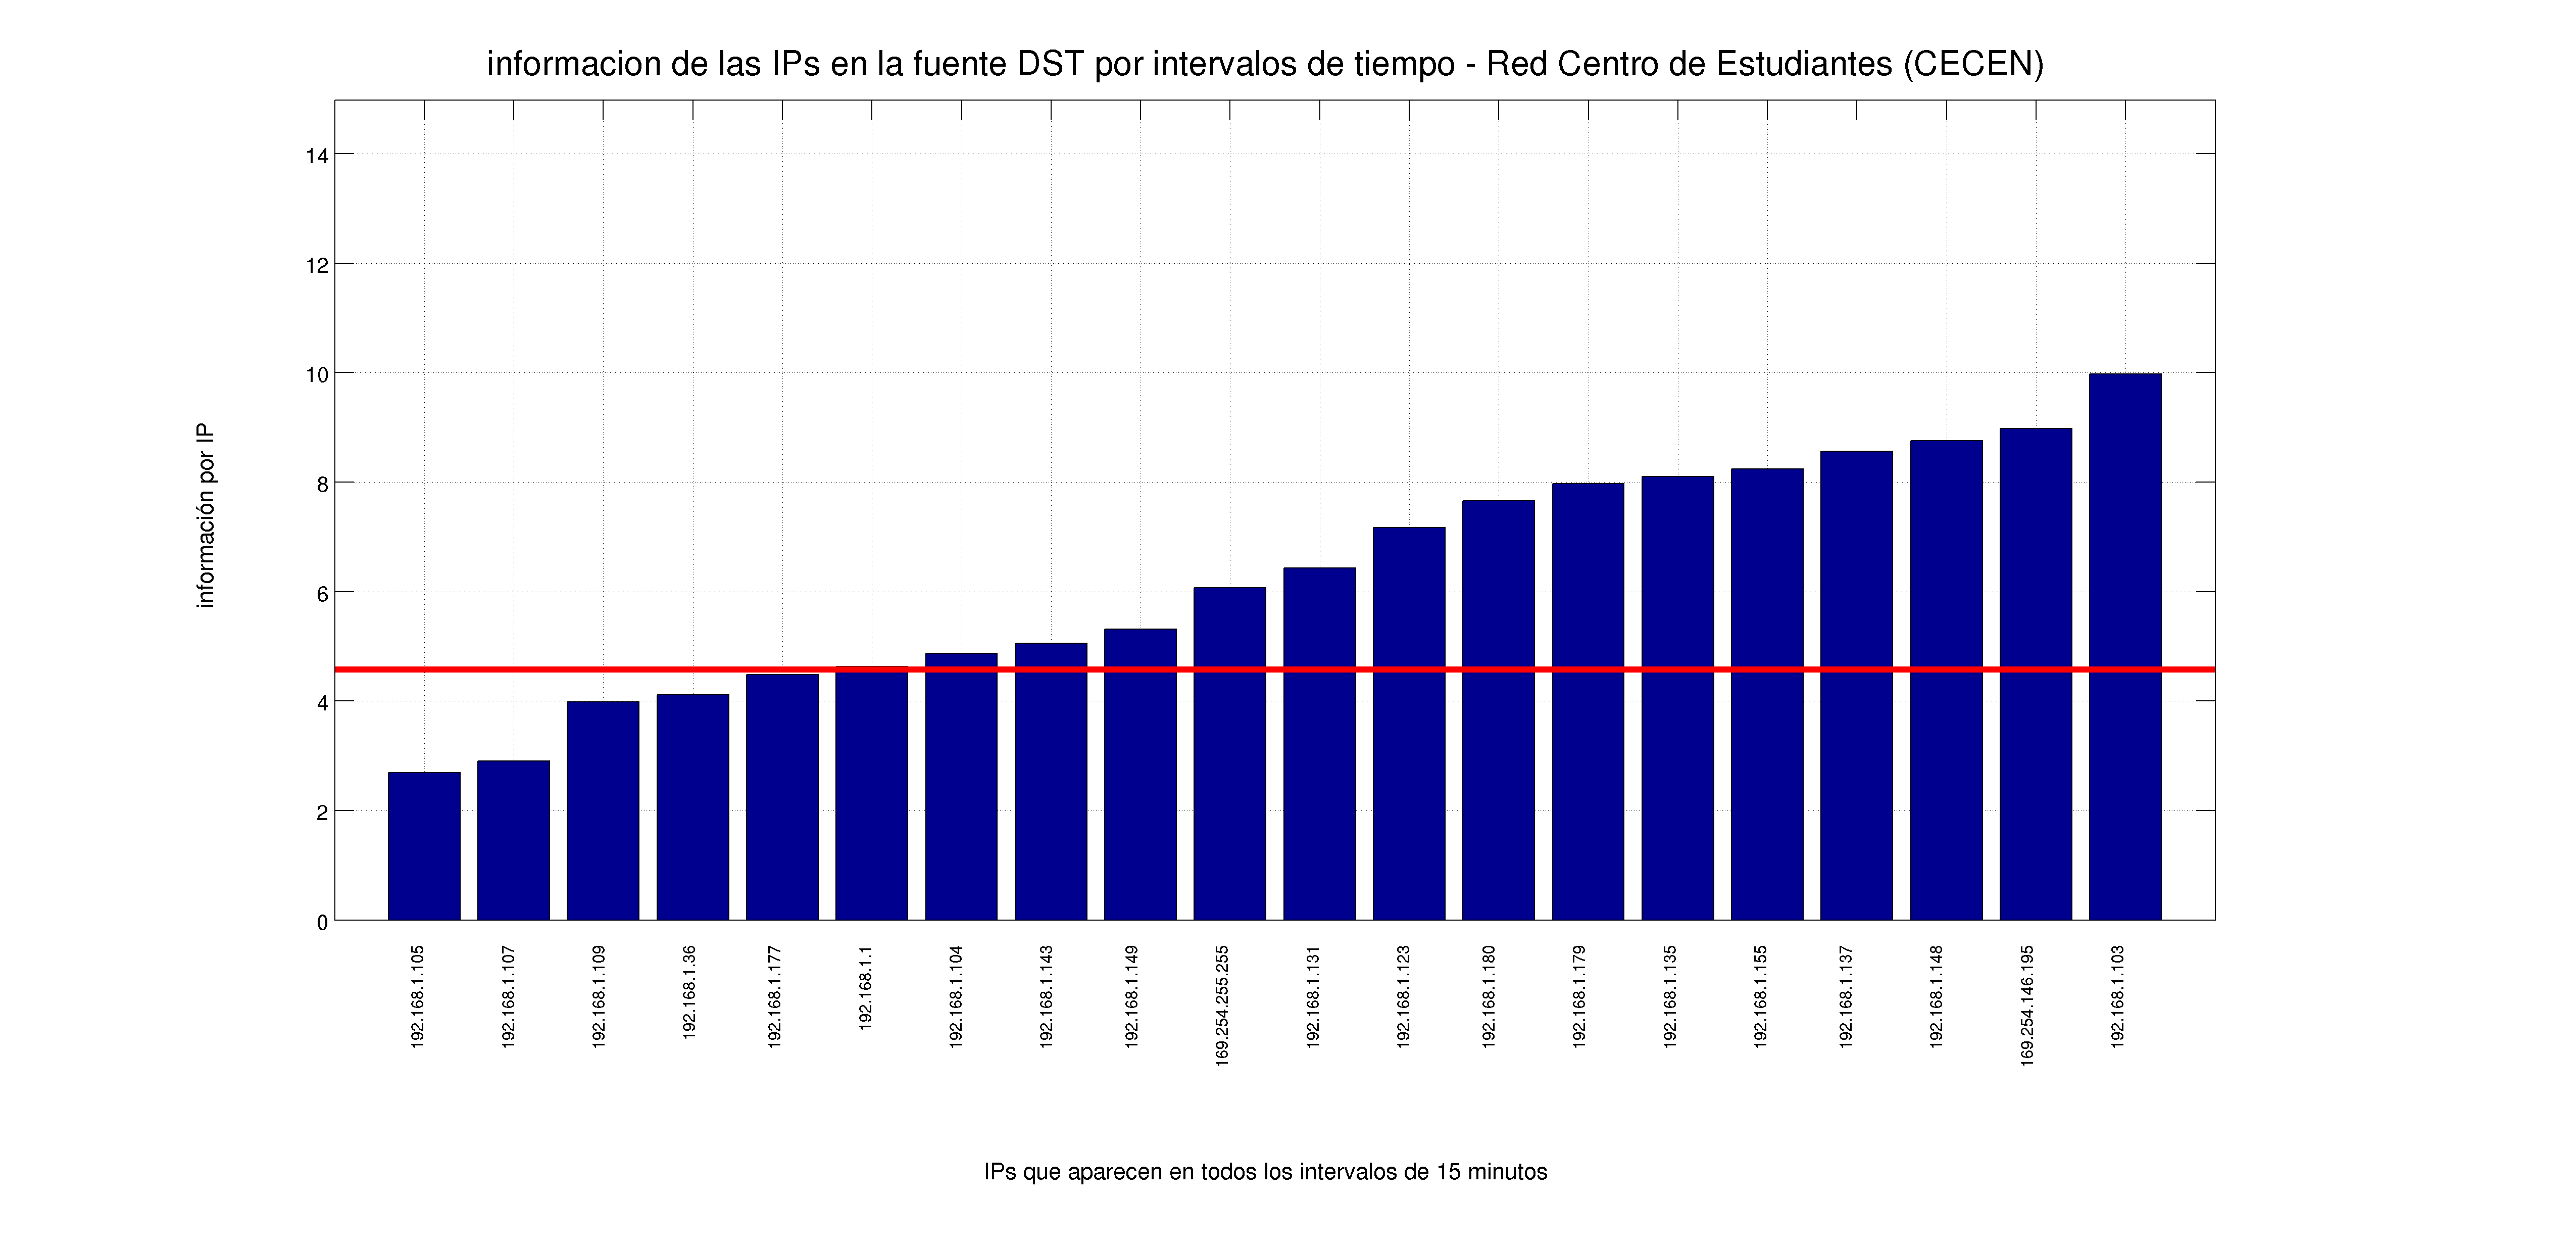
\includegraphics[width=\textwidth, trim=0 0 0 0]{../Graficos/cecen_infoConEn_dst_15.png}
\caption{Información y Entropía (rojo) - Fuente $S_{dst}$ - Red CECEN - Intervalos de 15 minutos. Las IPs mostradas son las que enviaron {\tt who-has} en todos los
intervalos de tiempo de dicha longitud, de la medición de 30 minutos.}
\end{figure}

\newpage
